\documentclass[a4paper,twoside,10pt]{book}

\usepackage[english]{babel}
\usepackage{float}
\usepackage{xparse}
\usepackage[utf8]{inputenc}
\usepackage{amsmath}
\usepackage{fancyhdr}
\usepackage{geometry}
\usepackage{pgfplots,pgfplotstable}
\usepackage{colortbl}
\usepackage[notoday,nofancy]{svninfo}

\usepackage[nottoc]{tocbibind}     %--- adds bibliography to toc 
% --- but without toc itself [nottoc] 
\usepackage[round,sort,comma,authoryear]{natbib} %--- creates bibliography; author-year with curly brackets within the text
% \usepackage[  %--- no numbering of positions 
% toc,           %--- let it appear in the document's table of contents
% style=mylong3colheader %--- see glossaries Documentation for a list of available styles
% ]{glossaries}  %--- use the glossary package
\geometry{a4paper,textwidth=15.8cm,textheight=23.0cm,twoside,rmargin=0.96in} %--- Variation Randbereiche
\usepackage{caption}
\usepackage{subcaption}  %--- simplifies putting pictures side by side
\usepackage{longtable}
\usepackage{multirow}
\usepackage{tabularx}
\usepackage{supertabular}
\usepackage{booktabs}    % to give tables a more professional look
\usepackage{rotating}    % rotate column labels
\usepackage{xcolor}
\usepackage{listings}
\usepackage{hyperref}    % ability to create hyperlinks within the document
\usepackage{vhistory}
\usepackage{tikz}
\usepackage{etex}
\usepackage{xargs}
\usepackage{xstring}
\usepackage{enumitem}
\usepackage[strict]{changepage} % for adjustwidth environment
\usepackage{framed}
\usepackage{array}
\usepackage[titletoc]{appendix}
\usepackage{soul}



% left-aligned fixed-width table column
\newcolumntype{P}[1]{>{\raggedright\arraybackslash}p{#1}}


% define some colors
\definecolor{darkred}{rgb}{0.5,0.,0.}
\definecolor{darkblue}{rgb}{0.,0.,0.6}
\definecolor{darkgreen}{rgb}{0.,0.5,0.}
\definecolor{darkgrey}{rgb}{0.7,0.75,0.71}
\definecolor{Gray}{gray}{0.9}

% textcolors
\newcommand{\tred}{\textcolor{red}}
\newcommand{\tblu}{\textcolor{blue}}
\newcommand{\degree}{{\circ}}
\newcommand{\km}{\text{km}}


% customize hyperref
\hypersetup{colorlinks, linkcolor=darkblue, citecolor=blue, urlcolor=darkred, linktoc=all}



% Fortran environment
\lstnewenvironment{fortran}%
{\lstset{language=[95]Fortran,%
    basicstyle=\ttfamily\footnotesize\color{darkgreen},%
    breaklines=true,%
    commentstyle=\ttfamily\color{blue},%
    emptylines=0,%
    keywordstyle=\color{black}\ttfamily\bfseries,%
    backgroundcolor=\color{darkgrey!5},
    framexleftmargin=4mm,%
    frame=shadowbox,%
    rulesepcolor=\color{darkgreen}}}
{}


% Sky environment
\lstnewenvironment{skydb}%
{\lstset{language=SQL,%
    basicstyle=\ttfamily\footnotesize\color{black},%
    breaklines=true,%
    commentstyle=\ttfamily\color{blue},%
    emptylines=0,%
    keywordstyle=\color{black}\ttfamily\bfseries,%
    backgroundcolor=\color{darkgrey!5},
    framexleftmargin=4mm,%
    frame=shadowbox,%
    rulesepcolor=\color{darkgreen}}}
{}

% LaTeX macros that are later used to disable/enable rows in the
% tables of output fields (global/local domain):
\newcommand{\onlyglb}[1]{#1}
\newcommand{\onlyloc}[1]{#1}

\newcommand{\new}[1]{}
\newcommand{\pressurelevelsTriangular}{}
\newcommand{\pressurelevelsRegular}{}
\newcommand{\heightlevelsRegular}{}


\newcolumntype{x}[1]{%
  >{\centering\hspace{0pt}}p{#1}}%


% ---------- Glossary: All the stuff and more ----------%
% \newglossary{symbolslist}{sym}{sbl}{Symbolverzeichnis} % define new glossary i.e. a list of symbols
% \makeglossaries

% \input{./text/listofsymbols}  %--- include defined symbols



% ---------------bold caption for figures-------------------------%
\makeatletter
\long\def\@makecaption#1#2{%
  \fontfamily{cmr}
  \fontseries{m}
  \fontshape{sl}
  \fontsize{10pt}{11pt}
  \selectfont
  \vskip 10\p@
  \setbox\@tempboxa\hbox{{\bf#1:} #2}%
  \ifdim \wd\@tempboxa >\hsize
  {\bf #1:} #2\par
  \else
  \hbox to\hsize{\hfil\box\@tempboxa\hfil}%
  \fi}
\makeatother
% ----------------------------------------------------------------%

% sign function
\newcommand{\sgn}{\operatorname{sgn}}

% \newcommand{\markRed}{\tikz \fill[red!60] (0,0) rectangle (0.08,0.8em);}
% \newcommand{\markBlue}{\tikz \fill[blue!80] (0,0) rectangle (0.08,0.8em);}
% \newcommand{\markWhite}{\tikz \fill[white!100] (0,0) rectangle (0.08,0.8em);}

\newcommand{\markRed}{
\begin{tikzpicture}[baseline,scale=0.15] 
                        \fill[red!60,draw=black] (0.1,0) -- (1,0) -- (1,1.7) -- cycle;
                        \fill[red!60,draw=black] (0,0.3) -- (0,2) -- (0.9,2) -- cycle;
                      \end{tikzpicture}}
\newcommand{\markBlue}{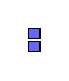
\begin{tikzpicture}[baseline,scale=0.15] 
                        \fill[blue!60,draw=black] (0,0)  rectangle ++(1,0.9);
                        \fill[blue!60,draw=black] (0,1.1) rectangle ++(1,0.9);
                      \end{tikzpicture}}
\newcommand{\markWhite}{\begin{tikzpicture}[baseline,scale=0.15] 
                        \fill[white!100,draw=white] (0.0,0) rectangle ++(1,2);
                      \end{tikzpicture}}


%% Macro for indicating whether field is available on native grid
%% (tri), lat-lon grid (ll), or both
%
% This is using LaTeX 3 to trim white space around macro arguments!
\newcommand{\groupsinner}[2]{
  \IfEqCase{#1}{%
      {tri}{%
           \IfEqCase{#2}{%
           {ll}{\markRed\hspace*{0.1em}\markBlue}}      %group (tri,ll)
           [\markRed\hspace*{0.1em}\markWhite]          %group (tri)
      }%
  }[%
           \IfEqCase{#2}{%
           {ll}{\markWhite\hspace*{0.1em}\markBlue}}     %group (ll)
  ]
}
%%% Now we go with LaTeX3
\ExplSyntaxOn
\NewDocumentCommand{\groups}{ O{none} O{none} }
 {
  \latex_groups_node:nn
   { \tl_trim_spaces:n { #1 } }
   { \tl_trim_spaces:n { #2 } }
 }
\cs_set_eq:NN \latex_groups_node:nn \groupsinner
\cs_generate_variant:Nn \latex_groups_node:nn { xx }
\ExplSyntaxOff

% width of column containing grid native/lon-lat marks
\newcommand{\markcolwidth}{0.50cm}
% longtable header settings
\newenvironment{vartable}[1]{%
\begin{longtable}{%
@{}p{\markcolwidth}%
@{\hskip 0.05in}%
p{2.0cm}%
>{\small\raggedright}p{5cm}<{\normalsize}%
p{0.5cm}%
p{0.5cm}%
p{0.5cm}%
p{1.4cm}p{1cm}p{1cm}}#1\\
  \toprule
&\multicolumn{1}{c}{\begin{sideways}\textbf{ShortName}\end{sideways}}  &  \multicolumn{1}{c}{\rb{\textbf{Description}}}  & \begin{sideways}\textbf{Discipline}\end{sideways} & \begin{sideways}\bf{Category}\end{sideways} & \begin{sideways}\bf{Number}\end{sideways}  & \begin{sideways}\bf{Lev-Typ 1/2}\end{sideways}  & \begin{sideways}\bf{stepType}\end{sideways} &\begin{sideways}\bf{Unit}\end{sideways}\\
\midrule

\endfirsthead
\caption[]{\emph{continued}}\\
\midrule
\endhead
\hline \multicolumn{8}{r}{\textit{Continued on next page}} \\
\endfoot
\endlastfoot
}%
{%
  \bottomrule
\end{longtable}}

%
%
% mark Namelists
% - im Fliesstext:
\newcommand{\nml}[1]{\texttt{#1}}



% environment derived from framed.sty: see leftbar environment definition
\definecolor{formalshade}{rgb}{0.95,0.95,1}

\newenvironment{note}{%
  \def\FrameCommand{%
    \hspace{1pt}%
    {\color{darkblue}\vrule width 2pt}%
    {\color{formalshade}\vrule width 4pt}%
    \colorbox{formalshade}%
  }%
  \MakeFramed{\advance\hsize-\width\FrameRestore}%
  \noindent\hspace{-4.55pt}% disable indenting first paragraph
  \begin{adjustwidth}{}{7pt}%
%  \vspace{-2pt}\vspace{-2pt}%
}
{%
  %\vspace{2pt}%
  \end{adjustwidth}\endMakeFramed%
}


%\parskip0.4ex plus0.2ex minus0.3ex
\setlength{\parskip}{0.2cm plus0.1cm minus0.1cm}
\setlength{\parindent}{0.0em}

\includeonly{./preface_title_toc,
             ./preface_intro,
             ./preface_versionhistory,
             ./analysis,
             ./input,
             ./grid_geometry,
             ./output_GRIB2_global,
             ./output_GRIB2_nest,
             ./icon_in_sky,
             ./appendix,
             ./output_statproc,
             ./output_description,
             ./quote,
             ./cosmo_eu_fields.tex} 



% ------------------ start of document -----------------------%
\begin{document}
\svnInfo $Id$
\setcounter{tocdepth}{3}     %--- maximum toc depth


\pagestyle{fancy}
\fancyhead{}
\fancyfoot{}
% --- Seitenzahl bei geraden/linken Seiten nach links/aussen
% --- Seitenzahl bei ungeraden/rechten Seiten nach rechts/aussen
\fancyhead[EL,OR]{\thepage}
% --- Kapitel/Abschnitt bei geraden/linken Seiten rechts/aussen
\fancyhead[ER]{\leftmark}
% --- Unterkapitel/Unterabschnitt bei ungeraden/rechten Seiten links/aussen
\fancyhead[OL]{\rightmark}

\renewcommand{\chaptermark}[1]{%
  \markboth{\chaptername
    \ \thechapter.\ #1}{}}

\renewcommand{\sectionmark}[1]{
  \markright{\thesection.\ #1}
}

% --- Erhoehung des vertikalen Abstandes zwischen den Zeilen eines Arrays
\renewcommand{\arraystretch}{1.5}

% --- Auswahl der Formatierung des Literaturverzeichnisses (deutsche Version), erstellt mit custom-bib package
% \bibliographystyle{plain}
% \bibliographystyle{diss_bibstyle.bst}
\bibliographystyle{jas99}

% --- search path for figures
\graphicspath{{./pics/}}
% ----------------------------------------------------------------%

\frontmatter     %--- aendert Zahlen von Arabisch auf roemisch

% ---------------- Generate title page ---------------------%
\begin{titlepage}
  \svnInfo $Id$
% --------------------------------------------------------------------------------
% Facsimile of DWD publication title page
% compliant with the specifications by J. Rapp, PB FB, 
% F. Prill, DWD: 2015-12-16.
%
% Changes wrt. MS Word layout
% - Font: "DejaVuSans" chosen as DWD's second corporate design font, instead of 
%   the MS Word layout which had been typeset in "Arial". The "Arial" font has
%   its primary use for computer monitors.
% - Compared to the MS Word layout, the capitalization "Research and Development"
%   has been chosen to match the headline style of the following line.
% - Corrected the list of authors: no "by", changed "und" to "and". First names
%   abbreviated.
% - Alignment of CC license description has been changed
% - Quotation marks in "Publisher" paragraph and on backside have been changed to 
%   English style
% --------------------------------------------------------------------------------

% ---------------- Generate title page ---------------------%
\thispagestyle{empty}
\begin{tikzpicture}[remember picture,overlay,transform shape] 
  % 
  \node[anchor=north east, xshift=-1.1cm, yshift=-1.1cm, scale=1.] at (current page.north east)
  {
\includegraphics[width=7.6cm]{Wortbildmarke-und-Claim-positiv-transparent.pdf}};
  % 
  \node[anchor=north west, xshift=3.25cm, yshift=-7cm, scale=1.4] at (current page.north west)
  {\begin{sansserif}%
      \textcolor{DWDblue}{Research and Development at DWD}
    \end{sansserif}};
  % 
  \node[anchor=north west, xshift=3.25cm, yshift=-8.25cm, scale=2.] at (current page.north west)
  {\begin{sansserif}%
      \textbf{ICON Database Reference Manual}
    \end{sansserif}};
  % 
  \node[anchor=north west, xshift=3.25cm, yshift=-9.6cm, scale=1.4] at (current page.north west)
  {\begin{sansserif}%
      \textbf{Version \vhCurrentVersion}
    \end{sansserif}};
  % 
  \node[anchor=north west, xshift=3.25cm, yshift=-10.5cm, scale=1.4] at (current page.north west)
  {\begin{sansserif}%
      Last changes: \svnInfoLongDate
    \end{sansserif}};
  % 
  \node[anchor=north west, xshift=3.25cm, yshift=-12.5cm, scale=1.4] at (current page.north west)
  {\begin{sansserif}%
      D.\ Reinert, F.\ Prill, H.\ Frank, and G.\ Z\"angl
    \end{sansserif}};
  % 
  \node[anchor=south west, xshift=3.25cm, yshift=5cm, scale=1.] at (current page.south west)
  {
\includegraphics[width=15cm]{icon_with_nest.png}};
  % 
  \node[anchor=south west, xshift=1.2cm, yshift=1.5cm, scale=1.] at (current page.south west)
  {
\includegraphics[width=1.5cm]{Bundesadler_schwarz.pdf}};
  % 
  \node[anchor=north west, xshift=3.25cm, yshift=3.0cm, scale=0.8] at (current page.south west)
  {\begin{sansserif}%
      Offenbach am Main, 2016
    \end{sansserif}};
\end{tikzpicture}
% ----------------------------------------------------------%


% ---------------- Back of title page ----------------------%
\newpage
\thispagestyle{empty}
\begin{tikzpicture}[remember picture,overlay,transform shape] 
  \node[anchor=north west, xshift=1.1cm, yshift=-18.5cm, scale=0.9] at (current page.north west)
  {\begin{sansserif}%
      \textbf{Version: \vhCurrentVersion}
    \end{sansserif}};
  % 
  \node[anchor=north west, xshift=1.1cm, yshift=-19.5cm, scale=0.9] at (current page.north west)
  {\begin{sansserif}%
      This document is based on Revision 20612 of the ICON code,
      last changed on \svnInfoDate.
    \end{sansserif}};
  % 
  \draw[black] ($(current page.north west)+(1.1cm,-20.7cm)$) -- ++ (18.4cm,0cm);
  % 
  \node[anchor=north west, xshift=1.1cm, yshift=-21.2cm, scale=0.9] at (current page.north west)
  %  Der DOI bildet sich aus
  %  1.       10.5676/DWD_    : für den ganzen DWD einheitlich
  %  2.       Pub/nwv/        : von PBFB für die FE1-Publikationen vorgegeben
  %  3.       Icon_0.8.3      : frei von FE1 wählbar
  {\begin{sansserif}%
      \detokenize{DOI: 10.5676/DWD_pub/nwv/icon_}\vhCurrentVersion
    \end{sansserif}};
  % 
  \node[anchor=north west, xshift=1.1cm, yshift=-22.95cm, scale=1.] at (current page.north west)
  {
\includegraphics[width=2.25cm]{by-nc-nd.pdf}};
  % 
  \node[anchor=north west, xshift=3.75cm, yshift=-23cm, scale=0.9] at (current page.north west)
  {\begin{sansserif}%
      \parbox{17.cm}{
        The CC license ``BY-NC-ND'' allows others only to download the publication and share it
        with others as long as they credit the publication, but they can't change it in any way 
        or use it commercially.
      }
  \end{sansserif}};
  % 
  \draw[black] ($(current page.north west)+(1.1cm,-24.75cm)$) -- ++ (18.4cm,0cm);
  % 
  \node[anchor=north west, xshift=1.1cm, yshift=-25.3cm, scale=0.9] at (current page.north west)
  {\begin{sansserif}%
    \parbox{8cm}{
      \textbf{Publisher} \\
      Deutscher Wetterdienst \\
      Business Area ``Research and Development'' \\
      Frankfurter Stra\ss e 135 \\
      63067 Offenbach \\
      www.dwd.de
    }
  \end{sansserif}};
  % 
  \node[anchor=north west, xshift=8.6cm, yshift=-25.3cm, scale=0.9] at (current page.north west)
  {\begin{sansserif}%
    \parbox{11cm}{
      \textbf{Editors} \\
      Daniel Reinert, FE13, \\
      \hspace*{2em} Tel. +49 (69) 8062-2060, daniel.reinert@dwd.de \\
      Helmut Frank, FE13, \\
      \hspace*{2em} Tel. +49 (69) 8062-2742, helmut.frank@dwd.de \\
      Florian Prill, FE13, \\
      \hspace*{2em} Tel. +49 (69) 8062-2727, florian.prill@dwd.de \\
    }
  \end{sansserif}};
\end{tikzpicture}
% ----------------------------------------------------------%



\newpage

\begin{versionhistory}\small%
  \vhEntry{0.1.0}{10.01.13}{DR|FP}{Generated preliminary list of available GRIB2 output fields}
  \vhEntry{0.2.0}{12.07.13}{DR|FP}{Added a short section describing the horizontal ICON grid. \texttt{AUMFL\_S}, \texttt{AVMFL\_S} added to the list of available output fields}
  \vhEntry{0.2.1}{15.07.13}{DR   }{Provide newly available output fields in tabulated form. Change levelType of 3D atmospheric fields from 105 (Hybrid) to 150 ( Generalized vertical height coordinate)}
  \vhEntry{0.2.2}{16.07.13}{FP   }{Short description of ICON's vertical grid.}
  \vhEntry{0.2.3}{25.09.13}{DR   }{Added description of available First Guess and analysis fields}
  \vhEntry{0.2.4}{17.12.13}{DR   }{Added description of external paramater fields}
  \vhEntry{0.3.0}{24.01.14}{DR   }{Added information about horizontal output grids}
  \vhEntry{0.3.1}{24.01.14}{DR   }{Added information about newly available output field \texttt{OMEGA}}
  \vhEntry{0.4.0}{22.05.14}{HF   }{Added SKY-database documentation}
  \vhEntry{0.4.1}{15.07.14}{DR   }{Some documentation on statistical processing and minor updates. New output fields \texttt{ASWDIR\_S}, \texttt{ASWDIFD\_S}, \texttt{ASWDIFU\_S}, \texttt{DTKE\_CON} }
  \vhEntry{0.4.2}{10.09.14}{DR   }{New output fields \texttt{CLCT\_MOD}, \texttt{CLDEPTH}}
  \vhEntry{0.5.0}{01.10.14}{DR   }{Description of IAU initialization method}
  \vhEntry{0.5.1}{15.10.14}{DR   }{Updated description of necessary input fields}
  \vhEntry{0.5.2}{31.10.14}{DR   }{Add full table with model half level heights}
  \vhEntry{0.6.0}{05.12.14}{DR   }{Add short introduction and fix some minor bugs}
  \vhEntry{0.6.1}{10.12.14}{DR   }{New output field \texttt{APAB\_S}}
  \vhEntry{0.7.0}{16.12.14}{DR   }{Revised documentation of time invariant fields and a couple of bug fixes}
  \vhEntry{0.7.2}{09.01.15}{DR   }{General GRIB2 description}
  \vhEntry{0.8.0}{15.01.15}{FP|DR}{Couple of bug fixes regarding the available fields on triangular and regular grids}
  \vhEntry{0.8.1}{16.01.15}{FP|DR}{List of pressure-level variables available on triangular grids}
  \vhEntry{0.8.2}{16.01.15}{FP   }{List of height-level variables available on regular grids}
  \vhEntry{0.8.3}{16.01.15}{DR   }{List of variables exclusively available for $VV=0$}
  \vhEntry{0.8.4}{06.02.15}{FP|DR}{Details of internal interpolation onto lon-lat grids. Details regarding output frequency.}
  \vhEntry{0.8.5}{18.02.15}{FP   }{Additional pressure levels for regular grid output.}
  \vhEntry{0.8.6}{23.02.15}{FP   }{Formula for computing non-zero topography level height.}
  \vhEntry{1.0.0}{23.02.15}{FP   }{Additional table of model full levels.}
  \vhEntry{1.0.1}{24.02.15}{DR   }{Update on available forecast runs and time span.}
  \vhEntry{1.0.2}{27.02.15}{FP   }{Added tables for grid point with maximum topo height.}
  \vhEntry{1.0.3}{13.03.15}{DR|FP}{Section on statistically processed fields.}
  \vhEntry{1.1.0}{15.04.15}{FP|DR}{Section on ICON EU nest (preliminary).}
  \vhEntry{1.1.1}{07.07.15}{HF   }{Added SMA list, list of half levels for EU nest, modified output lists to automatically write model level variables in the namelist templates.}
  \vhEntry{1.1.1}{17.07.15}{HF   }{Preliminary add T\_S because it is already written in operations. Some other minor modifications.}
  \vhEntry{1.1.2}{14.08.15}{FP   }{Added note on ICON's earth radius and a table summarizing regular grids.}
  \vhEntry{1.1.3}{04.12.15}{FP   }{Added WW code table~\ref{table:ww_code_table}.}
  \vhEntry{1.1.4}{11.01.15}{HF   }{Updated examples how to retrieve ICON data from SKY.}
\end{versionhistory}

\end{titlepage}
% ----------------------------------------------------------------%

%---- generate version history page -----------------%
\svnInfo $Id$
~
\vfill

This document is based on Revision 
\svnInfoMaxRevision\ of the ICON code,\\
Last changed on \svnInfoDate.

\begin{versionhistory}\small%
  \vhEntry{0.1.0}{10.01.13}{DR|FP}{Generated preliminary list of available GRIB2 output fields}
  \vhEntry{0.2.0}{12.07.13}{DR|FP}{Added a short section describing the horizontal ICON grid. \texttt{AUMFL\_S}, \texttt{AVMFL\_S} added to the list of available output fields}
  \vhEntry{0.2.1}{15.07.13}{DR   }{Provide newly available output fields in tabulated form. Change levelType of 3D atmospheric fields from 105 (Hybrid) to 150 ( Generalized vertical height coordinate)}
  \vhEntry{0.2.2}{16.07.13}{FP   }{Short description of ICON's vertical grid.}
  \vhEntry{0.2.3}{25.09.13}{DR   }{Added description of available First Guess and analysis fields}
  \vhEntry{0.2.4}{17.12.13}{DR   }{Added description of external paramater fields}
  \vhEntry{0.3.0}{24.01.14}{DR   }{Added information about horizontal output grids}
  \vhEntry{0.3.1}{24.01.14}{DR   }{Added information about newly available output field \texttt{OMEGA}}
  \vhEntry{0.4.0}{22.05.14}{HF   }{Added SKY-database documentation}
  \vhEntry{0.4.1}{15.07.14}{DR   }{Some documentation on statistical processing and minor updates. New output fields \texttt{ASWDIR\_S}, \texttt{ASWDIFD\_S}, \texttt{ASWDIFU\_S}, \texttt{DTKE\_CON} }
  \vhEntry{0.4.2}{10.09.14}{DR   }{New output fields \texttt{CLCT\_MOD}, \texttt{CLDEPTH}}
  \vhEntry{0.5.0}{01.10.14}{DR   }{Description of IAU initialization method}
  \vhEntry{0.5.1}{15.10.14}{DR   }{Updated description of necessary input fields}
  \vhEntry{0.5.2}{31.10.14}{DR   }{Add full table with model half level heights}
  \vhEntry{0.6.0}{05.12.14}{DR   }{Add short introduction and fix some minor bugs}
  \vhEntry{0.6.1}{10.12.14}{DR   }{New output field \texttt{APAB\_S}}
  \vhEntry{0.7.0}{16.12.14}{DR   }{Revised documentation of time invariant fields and a couple of bug fixes}
  \vhEntry{0.7.2}{09.01.15}{DR   }{General GRIB2 description}
  \vhEntry{0.8.0}{15.01.15}{FP|DR}{Couple of bug fixes regarding the available fields on triangular and regular grids}
  \vhEntry{0.8.1}{16.01.15}{FP|DR}{List of pressure-level variables available on triangular grids}
  \vhEntry{0.8.2}{16.01.15}{FP   }{List of height-level variables available on regular grids}
  \vhEntry{0.8.3}{16.01.15}{DR   }{List of variables exclusively available for $VV=0$}
  \vhEntry{0.8.4}{06.02.15}{FP|DR}{Details of internal interpolation onto lon-lat grids. Details regarding output frequency.}
  \vhEntry{0.8.5}{18.02.15}{FP   }{Additional pressure levels for regular grid output.}
  \vhEntry{0.8.6}{23.02.15}{FP   }{Formula for computing non-zero topography level height.}
  \vhEntry{1.0.0}{23.02.15}{FP   }{Additional table of model full levels.}
  \vhEntry{1.0.1}{24.02.15}{DR   }{Update on available forecast runs and time span.}
  \vhEntry{1.0.2}{27.02.15}{FP   }{Added tables for grid point with maximum topo height.}
  \vhEntry{1.0.3}{13.03.15}{DR|FP}{Section on statistically processed fields.}
  \vhEntry{1.1.0}{15.04.15}{FP|DR}{Section on ICON EU nest (preliminary).}
  \vhEntry{1.1.1}{07.07.15}{HF   }{Added SMA list, list of half levels for EU nest, modified output lists to automatically write model level variables in the namelist templates.}
  \vhEntry{1.1.1}{17.07.15}{HF   }{Preliminary add T\_S because it is already written in operations. Some other minor modifications.}
  \vhEntry{1.1.2}{14.08.15}{FP   }{Added note on ICON's earth radius and a table summarizing regular grids.}
\end{versionhistory}


% --------------------------------------------------------------------------------
\clearpage

\thispagestyle{empty}
\null\vfill

%\settowidth\longest{\huge\itshap}
\begin{center}
\parbox{0.75\textwidth}{%
  \raggedright{\Large\itshape%
  Simulations are believed by no one except those who conducted them.\\
  \par\bigskip
  Experimental results are believed by everyone except those who conducted them.\par\bigskip
  }   
  \raggedleft\large\MakeUppercase{Anonymous}\par%
}
\end{center}
\vfill\vfill

\clearpage
% --------------------------------------------------------------------------------

\newpage
\pdfbookmark{\contentsname}{toc}
\tableofcontents              %--- generate table of contents

% remove chapter number from header for abstracts
\renewcommand{\chaptermark}[1] {
  \markboth{#1}{}
}


% shifting table captions...
\newcommand{\rb}[1]{\raisebox{4.0ex}[0pt]{#1}}

% use default again
\renewcommand{\chaptermark}[1]{%
  \markboth{\chaptername
    \ \thechapter.\ #1}{}}

\mainmatter                   %--- Zurcksetzen der Nummerierung auf arabisch



% --------------------------------------------------------------------------------
% --------------------------------------------------------------------------------
\chapter{Introduction}
% --------------------------------------------------------------------------------

The \textbf{ICO}sahedral \textbf{N}onhydrostatic model ICON is the new global numerical 
weather prediction model at DWD. It became operational at 2015-01-20, replacing the former  
operational global model GME. The ICON modelling system as a whole is developed jointly by DWD and the 
Max-Planck Institute for Meteorology in Hamburg (MPI-M). While ICON is the new working horse 
for short and medium range global weather forecast at DWD, it will serve as the core of a new climate 
modelling system at MPI-M.

Since 2015-01-20, ICON analysis and forecast fields serve as initial and boundary data for
\begin{itemize}
 \item the regional model COSMO-EU
 \item RLMs (\textbf{R}elocatable \textbf{L}ocal \textbf{M}odel) of the German armed forces
 \item DWD's wave models
\end{itemize}

This document provides some basic information about ICON's horizontal and vertical grid structure, 
numerical algorithms (see also \cite{Zaengl15}) and physical parameterizations (the latter two are 
planned but not yet available). Furthermore, it provides an overview about the available ICON analysis 
and forecast fields stored in the data base SKY at DWD. Some examples on how to read these data from 
the data base are given as well.

\vfill
If you encounter bugs or inconsistencies, or if you have suggestions for improving this document, 
please contact one of the following colleagues:

\begin{note}
\begin{minipage}{\textwidth}
\centering
\begin{minipage}{0.32\textwidth}
 \textbf{Daniel Reinert}, FE13 \\
 Tel: +49 (69) 8062-2060 \\ 
 Mail: daniel.reinert@dwd.de
\end{minipage}
\begin{minipage}{0.32\textwidth}
 \textbf{Helmut Frank}, FE13\\
 Tel: +49 (69) 8062-2742 \\ 
 Mail: helmut.frank@dwd.de
\end{minipage}
\begin{minipage}{0.32\textwidth}
 \textbf{Florian Prill}, FE13 \\
 Tel: +49 (69) 8062-2727 \\ 
 Mail: florian.prill@dwd.de
\end{minipage}
\end{minipage}
\end{note}  
% --------------------------------------------------------------------------------

% --------------------------------------------------------------------------------
\svnInfo $Id$
% --------------------------------------------------------------------------------
\chapter{Grid geometry}
% --------------------------------------------------------------------------------


% --------------------------------------------------------------------------------
\section{Horizontal grid}
% --------------------------------------------------------------------------------

The horizontal ICON grid consists of a set of spherical triangles that seamlessly span the entire sphere. The grid is constructed from an icosahedron (see Figure 
\ref{fig_ico_a}) which is projected onto a sphere. The spherical icosahedron (Figure \ref{fig_ico_b}) consists of $20$ equilateral spherical triangles. The edges of each triangle 
are bisected into equal halves or more generally into $n$ equal sections. Connecting the new edge points by great circle arcs yields $4$ or more generally $n^2$ spherical triangles 
within the original triangle (Figure \ref{fig_bisect}, \ref{fig_nsect}). 

\begin{figure}[h]
  \begin{minipage}[b]{0.4\textwidth}
    \centering
    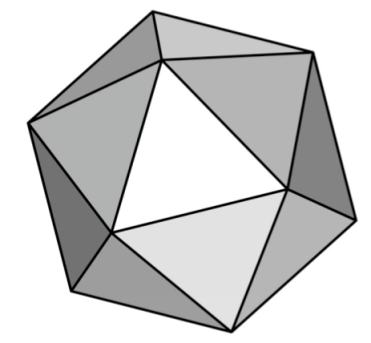
\includegraphics[width=0.69\textwidth]{icosahedron.png}
    \subcaption{}\label{fig_ico_a}
  \end{minipage}\hfill
  \begin{minipage}[b]{0.4\textwidth}
    \centering
    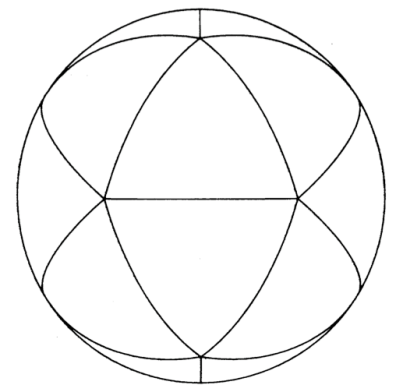
\includegraphics[width=0.69\textwidth]{icosahedron_spherical.png}
    \subcaption{}\label{fig_ico_b}
  \end{minipage}\hfill
  \caption{Icosahedron before (a) and after (b) projection onto a sphere }

\hfill

  \begin{minipage}[b]{0.4\textwidth}
    \centering
    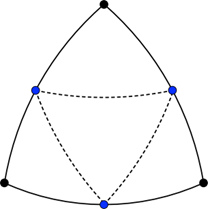
\includegraphics[width=0.69\textwidth]{bisection.png}
    \subcaption{}\label{fig_bisect}
  \end{minipage}\hfill
  \begin{minipage}[b]{0.4\textwidth}
    \centering
    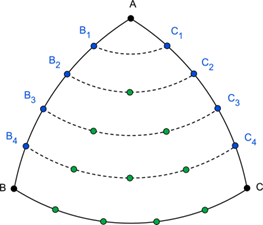
\includegraphics[width=0.78\textwidth]{nsection.png}
    \subcaption{}\label{fig_nsect}
  \end{minipage}\hfill
  \caption{(a) Bisection of the original triangle edges (b) More general division into $n$ equal sections}
\end{figure}

ICON grids are constructed by an initial root division into $n$ sections (\textbf{R}n) followed by $k$ bisection steps (\textbf{B}k), 
resulting in a \textbf{R}n\textbf{B}k grid. Figures \ref{fig_R2B00} and \ref{fig_R2B02} show \textbf{R}2\textbf{B}00 and 
\textbf{R}2\textbf{B}02 ICON grids. Such grids avoid polar singularities of latitude-longitude grids (Figure \ref{fig_lonlat}) 
and allow a high uniformity in resolution over the whole sphere.

\begin{figure}[h]
  \begin{minipage}[b]{0.3\textwidth}
    \centering
    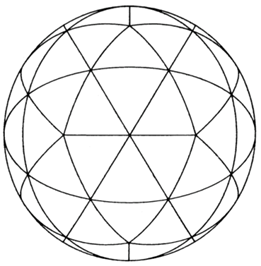
\includegraphics[width=0.9\textwidth]{icon_grid_R2B00.png}
    \subcaption{}\label{fig_R2B00}
  \end{minipage}\hfill
  \begin{minipage}[b]{0.3\textwidth}
    \centering
    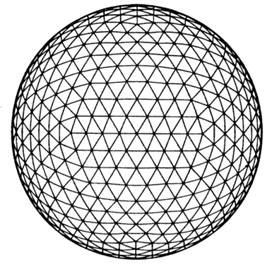
\includegraphics[width=0.95\textwidth]{icon_grid_R2B02.png}
    \subcaption{}\label{fig_R2B02}
  \end{minipage}\hfill
  \begin{minipage}[b]{0.3\textwidth}
    \centering
    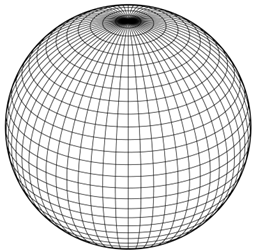
\includegraphics[width=0.95\textwidth]{lon-lat-grid.png}
    \subcaption{}\label{fig_lonlat}
  \end{minipage}\hfill
  \caption{(a) R2B00 grid. (b) R2B02 grid. (c) traditional regular latitude-longitude grid with polar singularities}
\end{figure}

Throughout this document, the grid is referred to as the ``\textbf{R}n\textbf{B}k grid'' or ``\textbf{R}n\textbf{B}k resolution''. For a given resolution \textbf{R}n\textbf{B}k, 
the total number of cells, edges, and vertices can be computed from
\begin{eqnarray*}
 n_{c} &=& 20\,n^{2}\,4^{k} \\
 n_{e} &=& 30\,n^{2}\,4^{k} \\
 n_{v} &=& 10\,n^{2}\,4^{k} + 2
\end{eqnarray*}
The average cell area $\overline{\Delta A}$ can be computed from
\begin{align*}
 \overline{\Delta A} = \frac{4\pi\,r_{e}^{2}}{n_{c}}\,,
\end{align*}
with the earth radius $r_{e}$, and $n_{c}$ the total number of cells. Based on $\overline{\Delta A}$ one can derive an estimate of the average grid resolution 
$\overline{\Delta x}$:
\begin{align*}
 \overline{\Delta x} = \sqrt{\overline{\Delta A}} = \sqrt{\frac{\pi}{5}} \frac{r_{e}}{n\,2^{k}}
\end{align*}
Visually speaking, $\overline{\Delta x}$ is the edge length of a square which has the same area as our triangular cell.


In Table \ref{tab_res}, some characteristics of frequently used ICON grids are given. The table contains information about the total number of triangles ($n_{c}$), the average 
resolution $\overline{\Delta x}$, and the maximum/minimum cell area. The latter may be interpreted as the area for which the prognosed meteorological quantities (like temperature, 
pressure, \dots) are representative. Some additional information about ICON's horizontal grid can be found in \citet{Wan13}.

\begin{table}[H]
  \caption{Characteristics of frequently used ICON grids. $\Delta A_{max}$ and $\Delta A_{min}$ refer to the maximum and minimum area of the grid cells, respectively.}\label{tab_res}
  \begin{center}
    \begin{tabular}{p{2.0cm}>{\raggedleft\arraybackslash}p{3.5cm}>{\centering\arraybackslash}p{3.5cm}>{\raggedleft\arraybackslash}p{2.5cm}>{\raggedleft\arraybackslash}p{2.5cm}}
    \toprule
    \textbf{Grid} & \textbf{number of cells ($n_{c}$)} & \textbf{avg.\ resolution [km]} & $\mathbf{\Delta A_{max}\,[km^{2}]}$ & $\mathbf{\Delta A_{min}\,[km^{2}]}$\\
    \midrule
    R2B04         &    20480                           &  157.8                         &  25974.2                  &  18777.3 \\
    R2B05         &    81920                           &   78.9                         &  6480.8                   & 4507.5\\
    R2B06         &   327680                           &   39.5                         &  1618.4                   & 1089.6 \\
    R2B07         &  1310720                           &   19.7                         &  404.4                    & 265.1 \\
    R3B07         &  2949120                           &   13.2                         &  179.7                    & 116.3 \\
    \bottomrule
    \end{tabular}
  \end{center}
\end{table}

\begin{note}
  \textbf{\textcolor{red}{The first operational version of ICON is
      based on the R3B07 grid, thus, having a horizontal resolution of
      about $13\,\mathrm{km}$!}}
\end{note}


% --------------------------------------------------------------------------------
\section{Vertical grid}
% --------------------------------------------------------------------------------

The vertical grid consists of a set of vertical layers with height-based vertical coordinates.
Each of these layers carries the horizontal $2D$ grid structure, thus forming the $3D$ structure of the grid.
The ICON grid employs a Lorenz-type staggering with the vertical velocity defined at the boundaries of layers (half levels) 
and the other prognostic variables in the center of the layer (full levels).

To improve simulations of flow past complex topography, the ICON model employs a smooth level vertical (SLEVE) coordinate~\citep{Leuenberger2010}. 
It allows for a faster transition to smooth levels in the upper troposphere and lower stratosphere, as compared to the classical height-based Gal-Chen 
coordinate. In the operational setup, the transition from terrain following levels in the lower atmosphere to constant height levels is completed 
at $z=16\,\mathrm{km}$. Model levels above are flat. The required smooth large-scale contribution of the model topography is generated by 
digital filtering with a $\nabla^2$-diffusion operator. Figure~\ref{fig:vertical_levels} shows the (half) levels of the planned operational 
ICON setup with 90 vertical levels. The table to the right shows the height above ground of selected half levels (for zero height topography) 
and the corresponding pressure, assuming the US standard atmosphere. Standard heights for all $91$ half levels are given in Table 
\ref{tab:half_level_heights}.

\textbf{Please note that for grid cells with non-zero topography these values only represent rough estimates of the true level height. Actual heights may 
vary considerably from location to location, due to grid level stretching/compression over non-zero topography.}
  
%In the operational setup, the transition from terrain following levels in the lower atmosphere to constant height levels is completed at 
%$z=16\,\mathrm{km}$. Model levels above are flat.



% ---------------------------------------------------------------------------------------
% ICON vertical levels -- SLEVE coordinates
% 
% author: 07/2013: F. Prill, DWD
% created with a Matlab script and the following settings:
%
%   min_lay_thckn   = 20.;        % Layer thickness of lowermost layer
%   top_height      = 75000.;     % Height of model top
%   stretch_fac     = 0.9;        % Scaling factor for stretching/squeezing 
%                                 % the model layer distribution
%   
%   decay_scale_1   = 4000.;      % Decay scale of large-scale topography component
%   decay_scale_2   = 2500.;      % Decay scale of small-scale topography component
%   decay_exp       = 1.2;        % Exponent for decay function
%   flat_height     = 16000.;     % Height above which the coordinate surfaces are flat
%   topo            = 0.;
%   topo_smt        = 0.;  
% 
% see also ICON routines "init_sleve_coord", "init_vert_coord"        
%
% Input files for this figure are created with the following commands:
%
%  octave -q --eval 'nlev=90; [z_m, z_i, pres_m, pres_i] = icon_levels(nlev); printf("k z p\n"); for k=1:nlev printf("%d %5.3f %5.3f\n",k,z_i(k),z_i(k)-z_i(k+1));end' > vertical_levels_i.txt 
%
%  octave -q --eval 'nlev=90; [z_m, z_i, pres_m, pres_i] = icon_levels(nlev); printf("k z p\n"); for k=[1:5:nlev,nlev] printf("%d %d %5.1f\n",k,z_i(k),pres_i(k));end' > vertical_levels_i_small.txt 
%
% (Alternatively, for a pressure plot:)
%  octave -q --eval 'nlev=90; [z_m, z_i, pres_m, pres_i] = icon_levels(nlev); printf("k z p\n"); for k=1:nlev printf("%d %5.3f %5.3f\n",k,z_i(k),pres_i(k));end' > vertical_levels_i.txt 
%
%
% ---------------------------------------------------------------------------------------
\begin{figure}[hb]
\begin{tabbing}
  \begin{minipage}[t]{0.65\linewidth} \vspace*{0pt}%
    \pgfplotstableread{level_tables/vertical_levels_i.txt}{\loadedtable}
    \pgfplotsset{
      tick label style={font=\small},
    }
  \begin{tikzpicture}[scale=0.7, transform shape]
    \begin{axis}[ minor tick num=1, axis x line=bottom, axis y line=left, 
                  every inner x axis line/.append style= {|->},
                  every inner y axis line/.append style= {|->}, 
                  width=10cm,height=14.5cm, ymajorgrids,
                  xlabel=level, 
                  scaled y ticks = false,
                  ylabel=\textbf{\color{blue}$z~\text{[m]}$}, enlargelimits=false,
                  every axis y label/.style={at={(current axis.north west)},
                                             yshift=3em,anchor=north east}
                ]
      \addplot[blue,mark=*] table[x={k},y={z}] \loadedtable;
    \end{axis}
    \begin{axis}[ minor tick num=1, axis x line=bottom, axis y line=right, 
                  every inner x axis line/.append style= {|->},
                  every inner y axis line/.append style= {|->}, 
                  width=10cm,height=14.5cm, 
                  scaled y ticks = false,
                  ylabel=\textbf{\color{red}$\Delta z~\text{[m]}$}, enlargelimits=false ,
                  every axis y label/.style={at={(current axis.north east)},
                                             yshift=3em,anchor=north west}
                 ]
      \addplot[red,only marks,mark=diamond] table[x={k},y={p}] \loadedtable;
    \end{axis}
  \end{tikzpicture}
  \end{minipage}
%
%
\=
%
%
  \begin{minipage}[t]{0.35\linewidth}\vspace*{0em}%
   \renewcommand{\baselinestretch}{0.95}\normalsize%
   \pgfkeys{/pgf/number format/set thousands separator={\,}}
   \pgfplotstableread{level_tables/vertical_levels_i_small.txt}{\loadedtablesmall}\vspace*{0pt}%
   \pgfplotstabletypeset[ columns={k,z,p},every  head row/.style={after row={\hline}},
          font=\footnotesize,
          columns/k/.style={column name=$level$, column type=r,column type/.add={>{\columncolor[gray]{.8}}}{}},
          columns/z/.style={column name=$[m]$,   fixed,dec sep align},
          columns/p/.style={column name=$[Pa]$, fixed,dec sep align, zerofill,precision=1},
                        ] {\loadedtablesmall}
    \vspace*{1em}%
  \end{minipage}
\end{tabbing}
%
  \caption{Vertical half levels (blue) and layer thickness (red) of the ICON operational setup.
    The table of selected pressure values (for zero height) is based on the 1976 US standard atmosphere.}
  \label{fig:vertical_levels}%
\end{figure}


% --------------------------------------------------------------------------------
\section{Refined subregion over Europe (``local nest'')}
% --------------------------------------------------------------------------------

ICON has the capability for running global simulations with refined
domains (so called \emph{nests}).
%
The triangular mesh of the refined area is generated by bisection of
triangles in the global ''parent'' grid, see
Fig.~\ref{fig:icon_grid_refinement_zoom_view}.
In the vertical the global grid extends into the mesosphere (which
greatly facilitates the assimilation of satellite data) whereas the
nested domains extend only into the lower stratosphere in order to
save computing time.
For each nesting level, the time step is automatically divided by a
factor of two.
%
Note that the grid nests are computed in a concurrent fashion:  Points
that are covered by the refined subdomain additionally contain data
for the global grid state.

\begin{figure}[h]
  \centering
  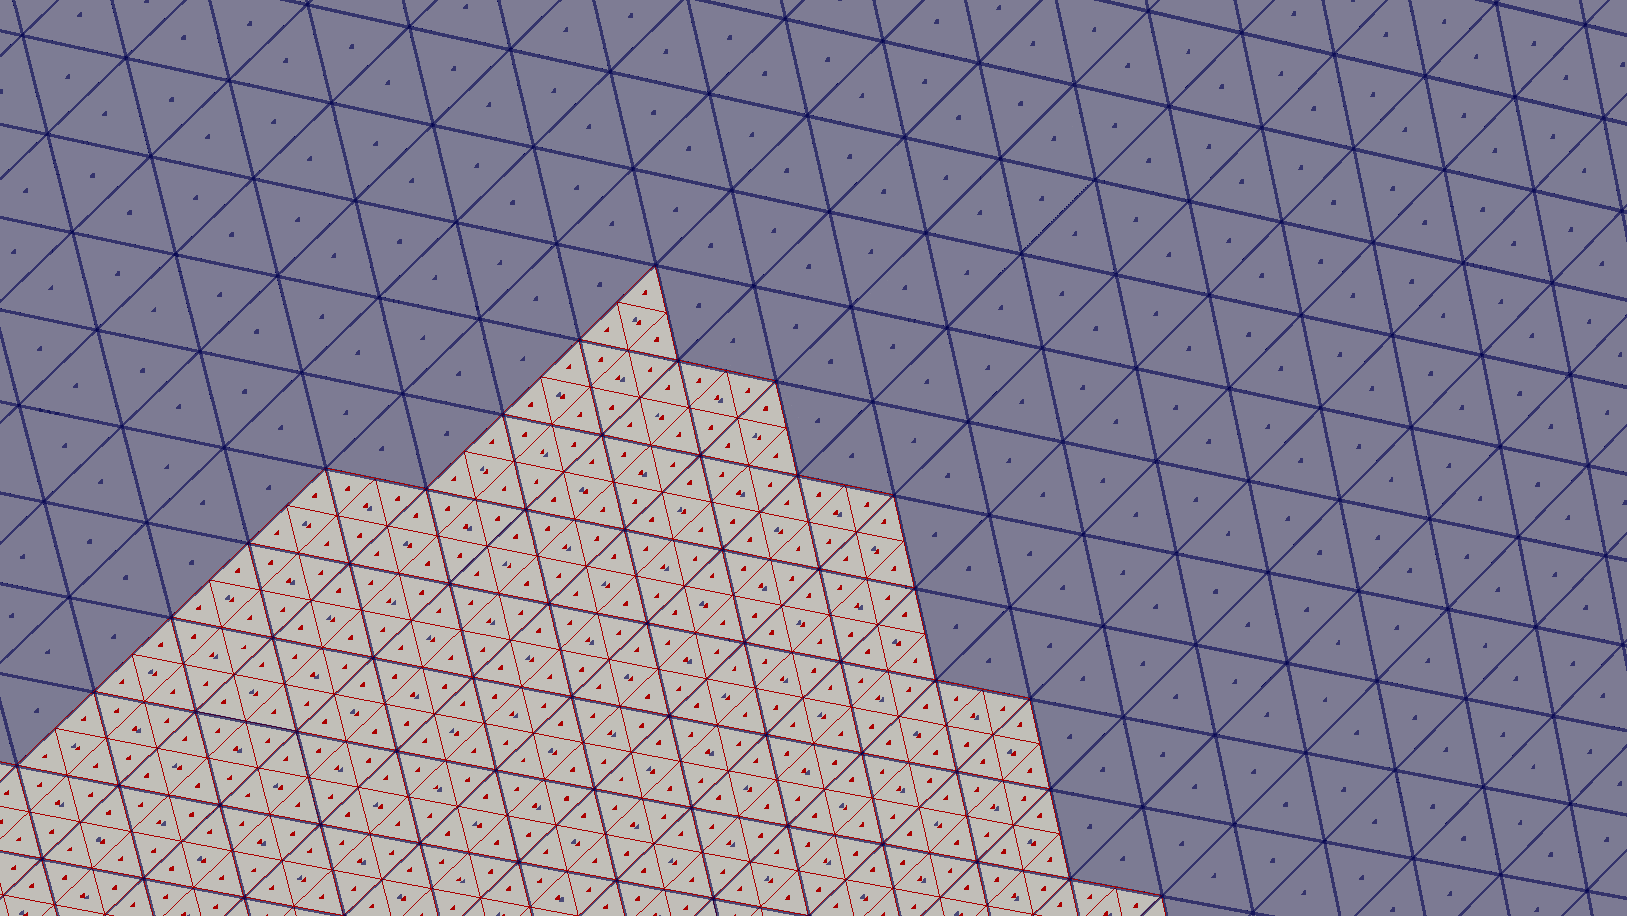
\includegraphics[width=0.90\textwidth]{pics/grid_refinement.png}
  \caption{ICON grid refinement (zoom view).}
  \label{fig:icon_grid_refinement_zoom_view}
\end{figure}



%  \begin{itemize}
%    \item No. of cells
%  \end{itemize}
%  
%  \begin{itemize}
%    \item Duplicate chapter on GRIB2 output tables for nest region
%    \item Description of IAU for nest
%    \item \emph{no} additional tables for HHL in appendix.
%  \end{itemize}



Currently, a refined subregion over Europe is in preparation,
which is comparable to the COSMO-EU region of DWD's COSMO model.

\begin{tabular}{|p{5cm}|l|l|}\hline
\rowcolor{Gray}
                           &    {\centering\textbf{ICON-EU nest}}                 &     {\centering\textbf{COSMO-EU}} \\ \hline\hline
% ----------------------------------------------------------------------------------------------------------------------------------------
geogr. coordinates         &    $23.5^\degree~\text{W}$ -- $62.5^\degree~\text{E}$    &     $\lambda_{\text{N}} = 170^\degree~\text{W}$, 
                                                                                          $\phi_{\text{N}}    =  40^\degree~\text{N}$,     \\
                           &    $29.5^\degree~\text{N}$ -- $70.5^\degree~\text{N}$   &      $18.0^\degree~\text{W} - 23.5^\degree~\text{E}$ \\
                           &                                                      &     $20.0^\degree~\text{S} - 21.0^\degree~\text{N}$  \\[0.5em]
mesh size                  &    $\approx 6.5~\km$ (R3B8)                          &     $0.0625^\degree$ ($\approx 7~\km$),  665 x 657 grid points \\
                           &    659156~triangles                                  & \\
vertical levels            &    60 levels                                         &     40 levels      \\
upper boundary             &    $22.5~\km$                                        &     $22.5~\km$ \\ \hline

\end{tabular}


\begin{note}
  \begin{center}
    \textbf{Model simulations including the nesting region over
      Europe will be run regularly starting from 2015-??-??.}
  \end{center}
\end{note}


Simulation on the global grid and the regional (Europe) domain are tightly coupled
(\emph{two-way nesting}):
Boundary data for the nest area is updated every time step (120~s).
%
Feedback of atmospheric prognostic variabes (except precipitation) is
computed via relaxation on a 3~h time scale.

  
\begin{figure}[h]
  \begin{minipage}[b]{\textwidth}
    \centering
    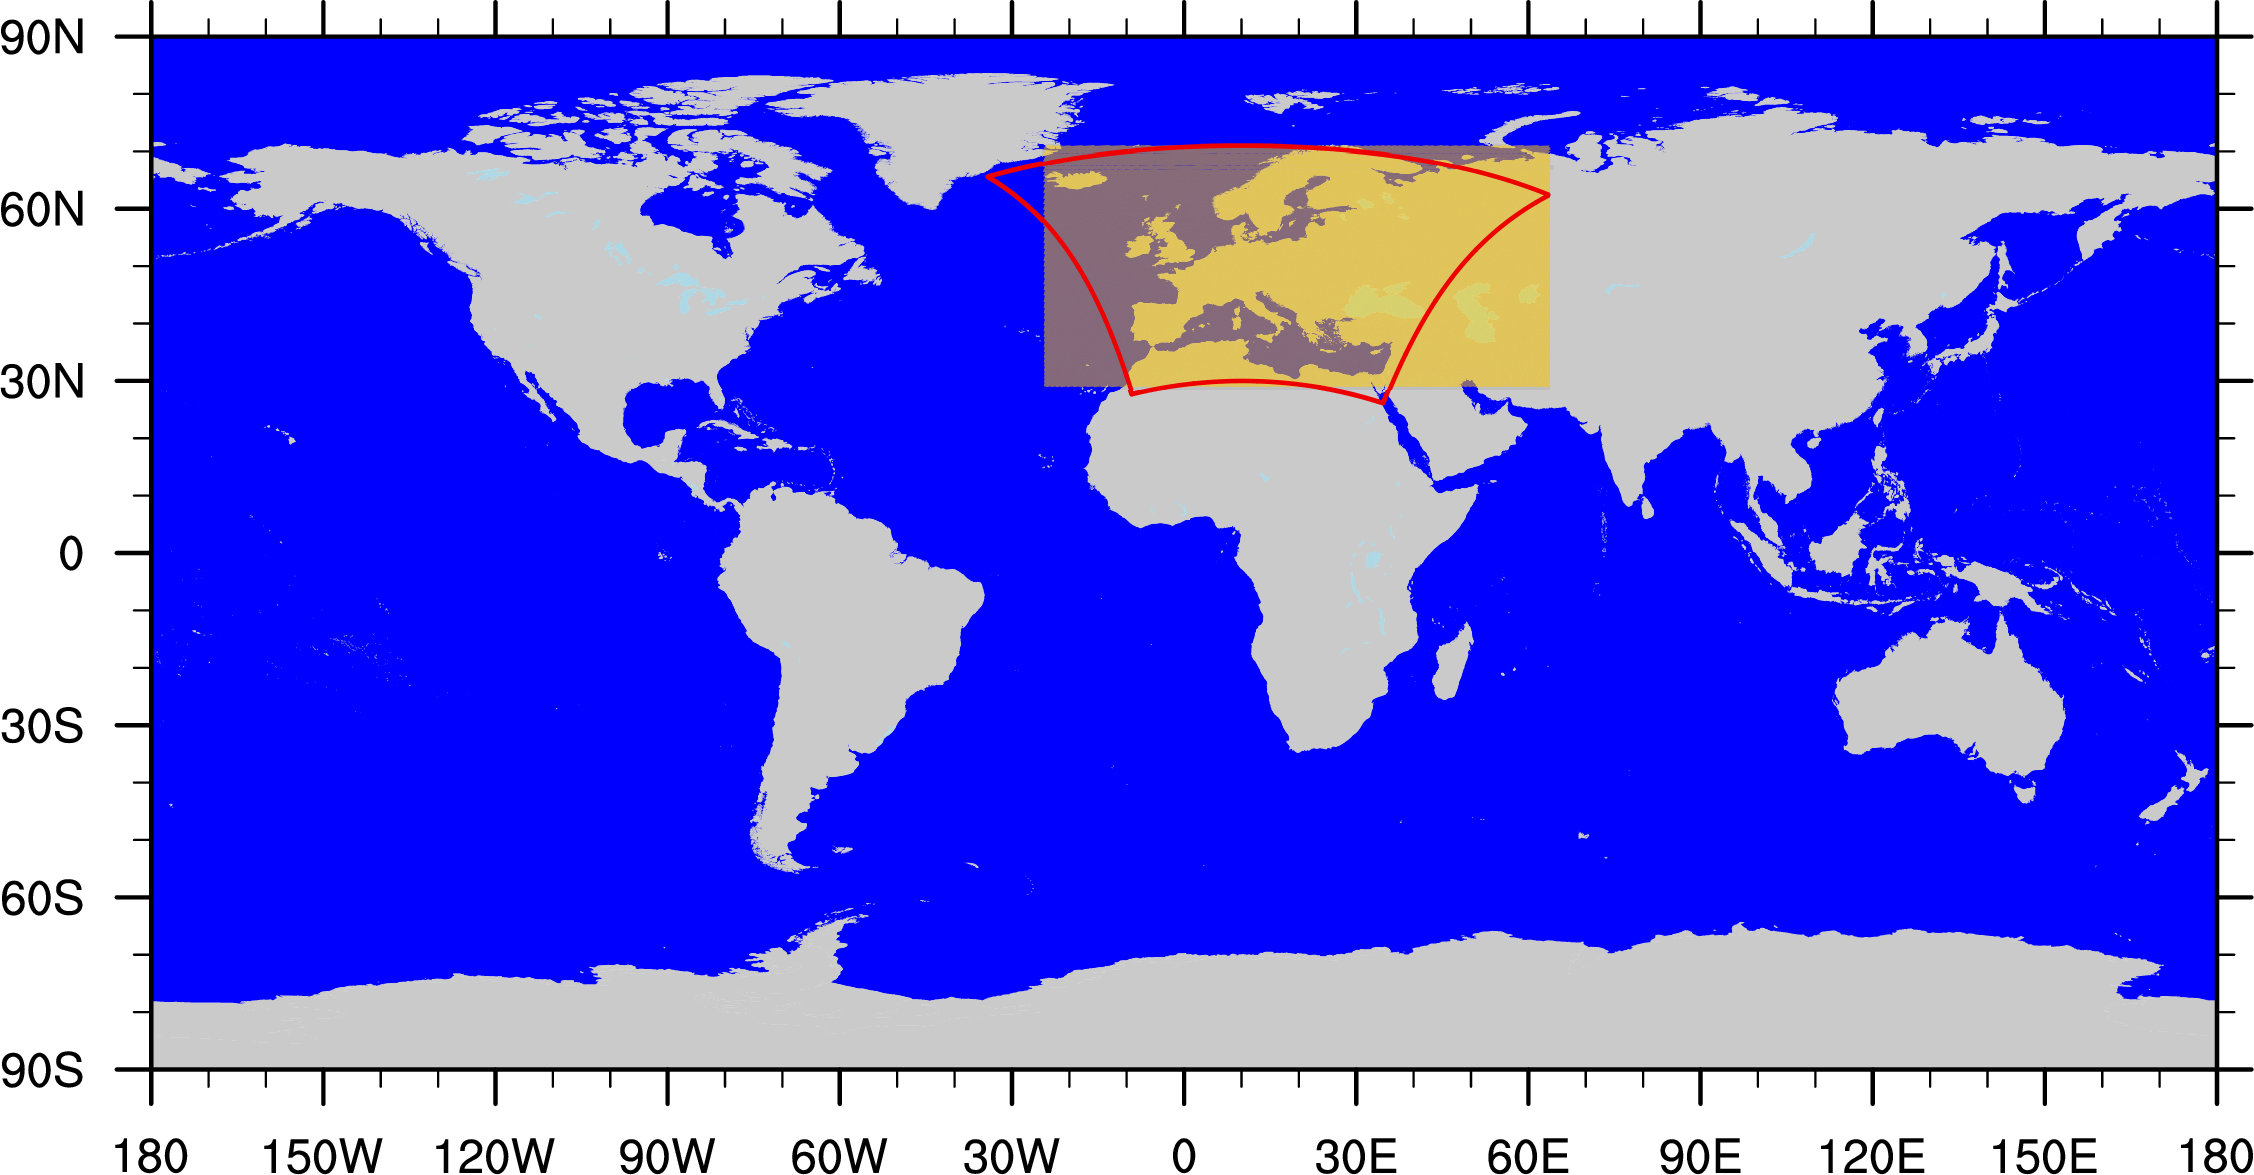
\includegraphics[width=0.90\textwidth]{ICON_EU_nest_1.png}
    \subcaption{}\label{fig:EU_nest}
  \end{minipage}
  \hfill
  \par
  \begin{minipage}[b]{\textwidth}
    \centering
    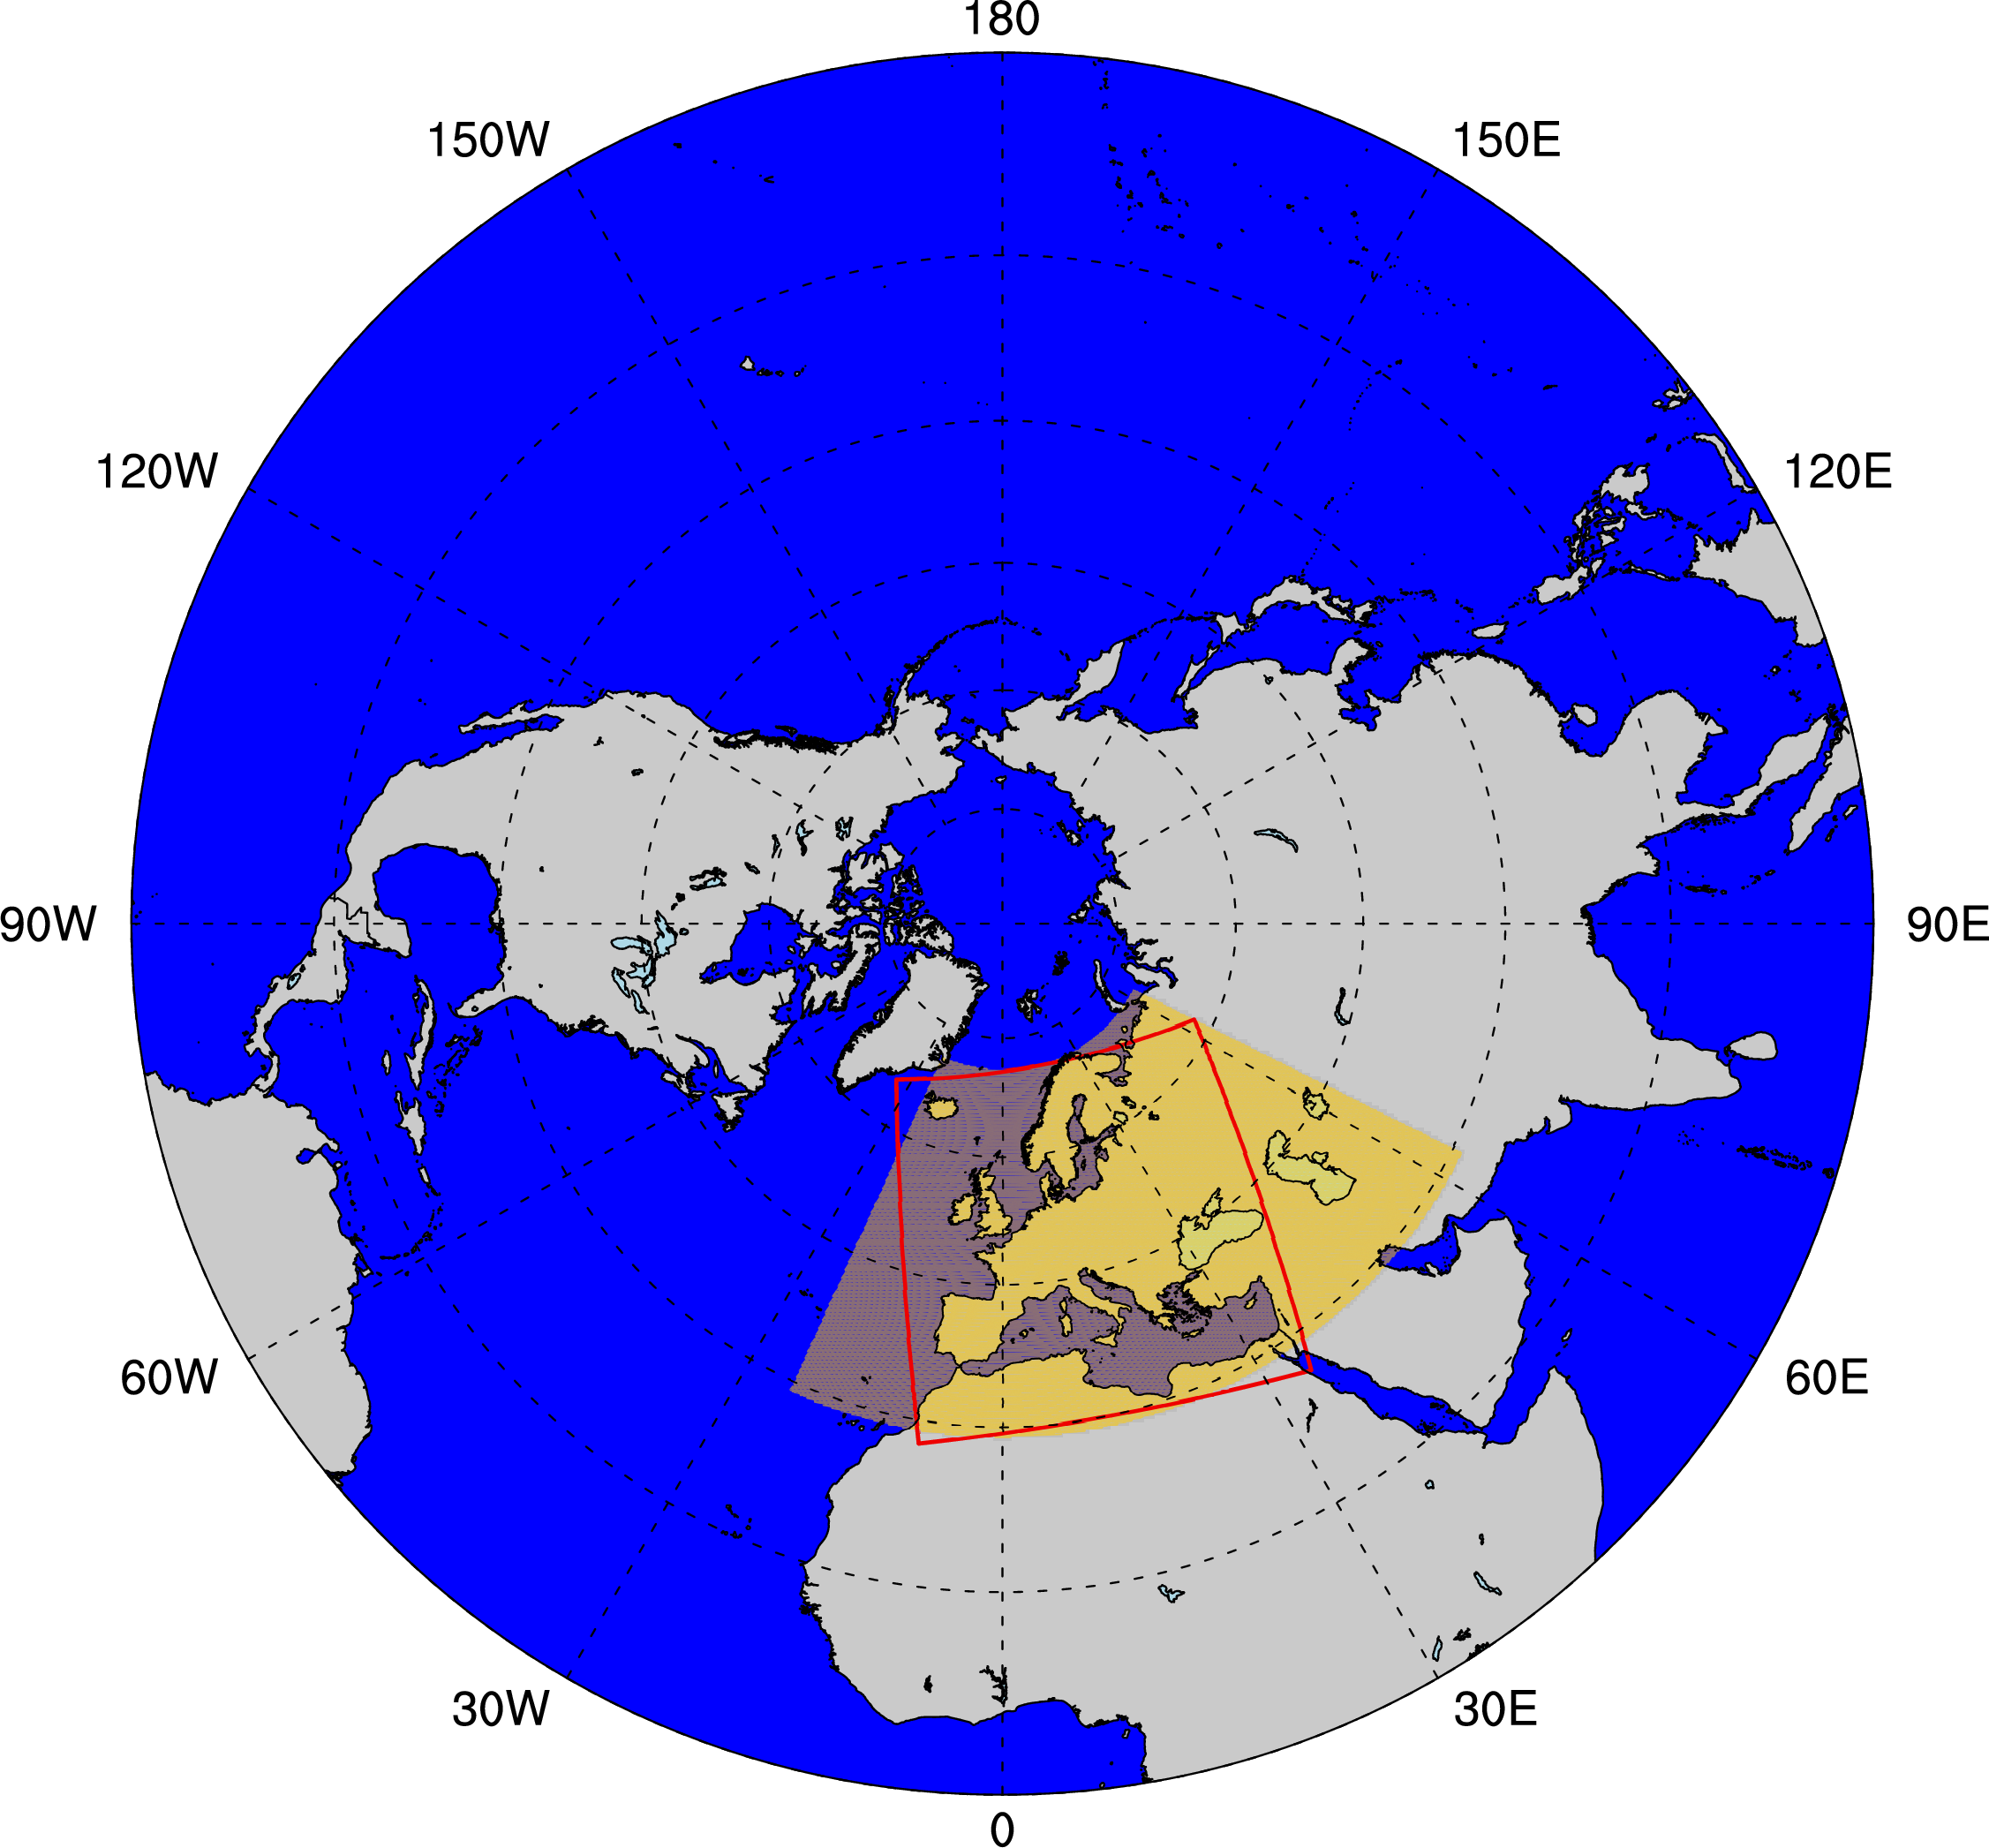
\includegraphics[width=0.80\textwidth]{ICON_EU_nest_2.png}
    \subcaption{}\label{fig:EU_nest_polar}
  \end{minipage}\hfill
  \caption{\ref{fig:EU_nest}: Horizontal extent of the ICON-EU nest
    (orange shaded area) in a cylindrical equidistant projection. For
    comparison, the outline of the COSMO-EU nest is shown in red.
    \ref{fig:EU_nest_polar}:  Same as \ref{fig:EU_nest} but in a polar
    stereographic projection.}
\end{figure}





% --------------------------------------------------------------------------------

% --------------------------------------------------------------------------------
\chapter{Mandatory input fields}

Several input files are needed to perform runs of the ICON model. 
%
These can be divided into three classes:
%
Grid files, external parameters, and initialization (analysis) files. The latter 
will be described in Chapter \ref{sec_analysis}.


%%%%%%%%%%%%%%%%%%%%%%%%%%%%%%%%%%%%%%%%%%%%%%%%%%%%%%%%%%%%%%%%%%%%%%%%%%%%%%%%%%%
\section{Grid Files}
\label{section:grid_files}

In order to run ICON, it is necessary to load the horizontal grid
information as an input para\-meter. 
This information is stored within so-called grid files. For an ICON 
run, at least one global grid file is required.
For model runs with nested grids, additional files of the nested
domains are necessary. Optionally, a reduced radiation grid for
the global domain may be used.

%
The unstructured triangular ICON grid resulting from the grid
generation process is represented in NetCDF format.  The most
important data entries are

\begin{itemize}
 \item \texttt{cell} (INTEGER dimension) \\
        number of (triangular) cells
 \item \texttt{vertex} (INTEGER dimension) \\
        number of triangle vertices
 \item \texttt{edge} (INTEGER dimension) \\
        number of triangle edges
 \item \texttt{clon}, \texttt{clat} (double array, dimension: \#triangles, given in radians) \\
        longitude/latitude of the triangle circumcenters
 \item \texttt{vlon}, \texttt{vlat} (double array, dimension: \#triangle vertices, given in radians) \\
        longitude/latitude of the triangle vertices
 \item \texttt{elon}, \texttt{elat} (double array, dimension: \#triangle edges, given in radians) \\
       longitude/latitude of the edge midpoints
 \item \texttt{cell\_area} (double array, dimension: \#triangles) \\
       triangle areas
 \item \texttt{vertex\_of\_cell} (INTEGER array, dimensions: [3, \#triangles]) \\
       The indices \texttt{vertex\_of\_cell(:,i)} denote the triangle vertices that belong 
       to the triangle~\texttt{i}.
 \item \texttt{edge\_of\_cell} (INTEGER array, dimensions: [2, \#triangles]) \\
       The indices \texttt{edge\_of\_cell(:,i)} denote the triangle edges that belong
       to the triangle~\texttt{i}.
\end{itemize}

%For fixed domain sizes and resolutions a list of grid files has been pre-built for the ICON model.
%These are publically available via the download server
%{\normalsize%
%\begin{verbatim}
%   http://icon-downloads.zmaw.de
%\end{verbatim}
%}%

%%%%%%%%%%%%%%%%%%%%%%%%%%%%%%%%%%%%%%%%%%%%%%%%%%%%%%%%%%%%%%%%%%%%%%%%%%%%%%%%%%%

\section{External parameters}
\label{section:extpar}
External parameters are used to describe the properties of the earth's surface. 
These data include the orography and the land-sea-mask. Also, several parameters
are needed to specify the dominant land use of a grid box like the soiltype
or the plant cover fraction.

The ExtPar software (ExtPar -- External parameter for Numerical Weather Prediction and Climate Application) 
is able to generate external parameters for the ICON model. The generation is based on a set of 
raw-datafields which are listed in Table \ref{table_extpar_raw}. For a more detailed overview of ExtPar, 
the reader is referred to the \emph{User and Implementation Guide} of Extpar.

\begin{longtable}{p{6.5cm}p{6cm}p{1.8cm}}
\caption[]{Raw datasets from which the ICON external parameter fields are derived.}\label{table_extpar_raw}\\
  \toprule
\textbf{Dataset} &\textbf{Source} &\textbf{Resolution} \\
\midrule
\endfirsthead
\caption[]{\emph{continued}}\\
\midrule
\endhead
\hline \multicolumn{3}{r}{\textit{Continued on next page}} \\
\endfoot
\endlastfoot
GLOBE orography                                        &  NOAA/NGDC                  &  30'' \\
%ASTER orography \newline (limited domain: 60 N - 60 S) &  METI/NASA                  &  1''   \\
GlobCover 2009                                         &  ESA                        &  10''  \\
%GLC2000 land use                                       &  JRC Ispra                  &  30''  \\
GLCC land use                                          &  USGS                       &  30''  \\
%DSMW Digital Soil Map of the World                     &  FAO                        &  5'    \\
HWSD Harmonized World Soil Database                    &  FAO/IIASA/ISRIC/ISSCAS/JRC &  30''  \\
NDVI Climatotology, SeaWiFS                            &  NASA/GSFC                  &  2.5'  \\
CRU near surface climatology                           &  CRU University of East Anglia & $0.5^{\circ}$  \\
GACP Aerosol Optical thickness                         &  NASA/GISS \newline (Global Aerosol Climatology Project)   &  $4x5^{\circ}$ \\
GLDB Global lake database                              &  DWD/RSHU/MeteoFrance       &  30''  \\
MODIS albedo                                           &  NASA                       &  5'    \\
\bottomrule
\end{longtable}

\emph{GlobCover 2009} is a land cover database covering the whole globe, except for Antarctica. Therefore, we make use of 
\emph{GlobCover 2009} for $90^{\circ} > \phi > -56^{\circ}$ (with $\phi$ denoting latitude) and switch to the coarser, 
however globally available dataset \emph{GLCC} for $ -56^{\circ} \geq \psi > -90^{\circ}$.

The products generated by the ExtPar software package are listed in Table \ref{table_extpar_products} together with the underlying 
raw dataset. Note that these are mandatory input fields for assimilation- and forecast runs.

\begin{longtable}{p{2.5cm}p{8.5cm}p{3.3cm}}
\caption[]{External parameter fields for ICON, produced by the ExtPar software package (in alphabetical order)}\label{table_extpar_products}\\
% \begin{tabular}{p{2.5cm}p{8.5cm}p{3.3cm}}
  \toprule
\multicolumn{1}{c}{\textbf{ShortName}}  &  \multicolumn{1}{c}{\textbf{Description}}  &  \multicolumn{1}{c}{\textbf{Raw dataset}}\\
\midrule
\endfirsthead
\caption[]{\emph{continued}}\\
\midrule
\endhead
\hline \multicolumn{3}{r}{\textit{Continued on next page}} \\
\endfoot
\endlastfoot
  AER\_SS12                             & Sea salt aerosol climatology (monthly fields)   &       GACP                \\
  AER\_DUST12                           & Total soil dust aerosol climatology (monthly fields) &  GACP                \\
  AER\_ORG12                            & Organic aerosol climatology (monthly fields)       &    GACP                \\
  AER\_SO412                            & Total sulfate aerosol climatology (monthly fields) &    GACP                \\
  AER\_BC12                             & Black carbon aerosol climatology (monthly fields)  &    GACP                \\
  ALB\_DIF12                            & Shortwave ($0.3 - 5.0\, \mathrm{\mu m}$) albedo for diffuse radiation (monthly fields)&  MODIS    \\
  ALB\_UV12                             & UV-visible ($0.3 - 0.7\, \mathrm{\mu m}$) albedo for diffuse radiation (monthly fields)& MODIS     \\
  ALB\_NI12                             & Near infrared ($0.7 - 5.0\, \mathrm{\mu m}$) albedo for diffuse radiation (monthly fields)& MODIS     \\
  DEPTH\_LK                             & Lake depth                                      &        GLDB               \\
  EMIS\_RAD                             & Surface longwave (thermal) emissivity           &        GlobCover 2009     \\               
  FOR\_D  (*)                           & Fraction of deciduous forest                    &        GlobCover 2009     \\
  FOR\_E  (*)                           & Fraction of evergreen forest                    &        GlobCover 2009     \\
  FR\_LAKE                              & Lake fraction (fresh water)                     &        GLDB               \\                     
  FR\_LAND                              & Land fraction (excluding lake fraction but including glacier fraction) & GlobCover2009   \\
  FR\_LUC                               & Landuse class fraction                          &                           \\
  HSURF                                 & Orography height at cell centres                &        GLOBE              \\
  LAI\_MX  (*)                          & Leaf area index in the vegetation phase         &        GlobCover 2009     \\
  NDVI\_MAX                             & Normalized differential vegetation index        &        SeaWiFS            \\
  NDVI\_MRAT                            & proportion of monthly mean NDVI to yearly maximum (monthly fields)&  SeaWiFS \\
  PLCOV\_MX  (*)                        & Plant covering degree in the vegetation phase   &        GlobCover 2009     \\
  ROOTDP (*)                            & Root depth                                      &        GlobCover 2009     \\
  RSMIN  (*)                            & Minimum stomatal resistance                     &        GlobCover 2009     \\
  SOILTYP                               & Soil type                                       &        HWSD               \\
  SSO\_STDH                             & Standard deviation of sub-grid scale orographic height  &   GLOBE           \\
  SSO\_THETA                            & Principal axis-angle of sub-grid scale orography &          GLOBE           \\
  SSO\_GAMMA                            & Horizontal anisotropy of sub-grid scale orography &         GLOBE           \\
  SSO\_SIGMA                            & Average slope of sub-grid scale orography       &           GLOBE           \\
  T\_2M\_CL                             & Climatological 2m temperature (serves as lower boundary condition for soil model)  &  CRU \\
  Z0 (*)                                & Surface roughness length (over land), containing a contribution from subgrid-scale orography  & GlobCover 2009    \\                        
  \bottomrule
% \end{tabular}
\end{longtable}

Note that fields marked with (*) are not required in operational model runs. I.e.\ the surface roughness \texttt{Z0} is only needed, 
if the additional contribution from sub-grid scale orography is taken into account (i.e.\ for \nml{itype\_z0=1}). In operational runs, land-cover 
class specific roughness lengths are taken from a GlobCover-based lookup table. \texttt{FOR\_D}, \texttt{FOR\_E}, \texttt{LAI\_MX}, \texttt{PLCOV\_MX}, 
\texttt{RSMIN}, and \texttt{ROOTDP} became obsolete with the activation of the surface tile approach (2015-03-04). The latter $4$ fields 
are replaced by land-cover class specific values taken from lookup tables.



\subsubsection*{Remarks on post-processing}
Some of the external parameter fields produced by ExtPar are modified by ICON. The following fields are affected: \texttt{DEPTH\_LK}, 
\texttt{HSURF}, \texttt{FR\_LAND}, \texttt{FR\_LAKE}, \texttt{Z0}. Thus, for consistency reasons, the modified fields should be used 
for post-processing tasks rather than the original external parameter fields.

% --------------------------------------------------------------------------------

% --------------------------------------------------------------------------------

\chapter{Analysis fields}\label{sec_analysis}

Numerical weather prediction (NWP) is an initial value problem. The ability to make a skillful forecast 
relies heavily on an accurate estimate of the present atmospheric state, known as the analysis.
In general, an analysis is generated by optimally combining all available observations with a short-range model 
forecast, known as \emph{first guess} (FG) or \emph{background}. Currently an atmospheric analysis is created 
every $3\,\mathrm{h}$. The 3-hourly first guess output provided by ICON comprises the following fields:
\begin{longtable}{p{4.0cm}P{7.0cm}}
\captionabove[]{Available $3\,\mathrm{h}$ first guess output fields from the forecast database 
\texttt{CAT\_NAME=\$model\_ass\_fc\_\$suite}}\\
  \toprule
\multicolumn{1}{c}{\textbf{Type}}  &  \multicolumn{1}{c}{\textbf{GRIB shortName}}\\
\midrule
\endfirsthead
\caption[]{\emph{continued}}\\
\midrule
\endhead
\hline \multicolumn{2}{r}{\textit{Continued on next page}} \\
\endfoot
\endlastfoot
Atmosphere                             &  VN, U, V, W, DEN, THETA\_V, T, QV, QC, QI, QR, QS, TKE, P                     \\
Surface (general)                      &  T\_G, T\_SO(0), QV\_S, T\_2M, TD\_2M, U\_10M, V\_10M, PS, Z0                       \\
Land specific                          &  W\_SNOW, T\_SNOW, RHO\_SNOW, H\_SNOW, FRESHSNW, W\_I, T\_SO(1:nlev\_soil), W\_SO, W\_SO\_ICE \\
Lake/sea ice specific                  &  T\_MNW\_LK, T\_WML\_LK, H\_ML\_LK, T\_BOT\_LK, C\_T\_LK, T\_B1\_LK, H\_B1\_LK, T\_ICE, H\_ICE, FR\_ICE\\
Time invariant                         &  FR\_LAND, HHL, CLON, CLAT, ELON, ELAT, VLON, VLAT \\
  \bottomrule
\end{longtable}

Atmospheric analysis fields are computed every 3 hours ($00$, $03$, $06$,$\dots$ $21$ UTC) by the 3DVar data assimilation system, 
which has recently been upgraded to an En-Var system (see Section \ref{sec:EDA}). Sea surface 
temperature \texttt{T\_SO(0)} and sea ice cover \texttt{FR\_ICE} are provided once per day (00 UTC) by the SST-Analysis. A snow analysis is 
conducted every 3 hours, providing updated information on the snow height \texttt{H\_SNOW} and snow age \texttt{FRESHSNW}. In addition a soil 
moisture analysis (SMA) is conducted once per day (00 UTC). It basically modifies the soil moisture content \texttt{W\_SO}, in order to improve 
the $2\,\mathrm{m}$ temperature forecast. 

 
For the 3-hourly assimilation cycle and forecast runs, ICON must be provided with $2$ input files: One containing the First Guess~(FG) and the other 
containing analysis~(AN) fields, only. Variables for which no analysis is available are always read from the first guess file (e.g.\ TKE). 
Other variables may be read either from the first guess or the analysis file, depending on the starting time. E.g.\ for T\_SO(0) the first 
guess is read at 03, 06, 09, 12, 15, 18, 21 UTC, however, the analysis is read at 00 UTC when a new SST analysis is available. 
In Table~\ref{tbl_analysis} the available and employed first guess and analysis fields are listed as a function of starting time.

\begin{longtable}{p{3.3cm}>{\centering\arraybackslash}p{2.5cm}p{0.7cm}p{0.7cm}p{0.7cm}p{0.7cm}p{0.7cm}p{0.7cm}p{0.7cm}p{0.7cm}}
\captionabove[]{The leftmost column shows variables that are mandatory for the assimilation cycle and forecast runs.  Column 2 indicates, whether or not an analysis is performed 
for these variables. Columns 3 to 10 show the origin of these variables (analysis or first guess), depending on the starting time.}\label{tbl_analysis}\\
  \toprule
\textbf{ShortName}  &  \textbf{Analysis}  & \textbf{00} & \textbf{03} & \textbf{06} & \textbf{09} & \textbf{12} & \textbf{15} & \textbf{18} &  \textbf{21} \\
\midrule
\endhead
\hline \multicolumn{10}{r}{\textit{Continued on next page}} \\
\endfoot
\endlastfoot
\hline \multicolumn{10}{l}{\textbf{Atmosphere}} \\
VN                  &     --              &   FG         &     FG      &     FG      &     FG      &     FG      &     FG      &     FG      &    FG         \\
THETA\_V            &     --              &   FG         &     FG      &     FG      &     FG      &     FG      &     FG      &     FG      &    FG         \\
DEN                 &     --              &   FG         &     FG      &     FG      &     FG      &     FG      &     FG      &     FG      &    FG         \\
W                   &     --              &   FG         &     FG      &     FG      &     FG      &     FG      &     FG      &     FG      &    FG         \\
TKE                 &     --              &   FG         &     FG      &     FG      &     FG      &     FG      &     FG      &     FG      &    FG         \\
QC, QI, QR, QS      &     --              &   FG         &     FG      &     FG      &     FG      &     FG      &     FG      &     FG      &    FG         \\
QV                  &     3DVar           &   \tred{AN}  &  \tred{AN}  &  \tred{AN}  &   \tred{AN} &   \tred{AN} &  \tred{AN}  &  \tred{AN}  &  \tred{AN}    \\
T                   &     3DVar           &   \tred{AN}  &  \tred{AN}  &  \tred{AN}  &   \tred{AN} &   \tred{AN} &  \tred{AN}  &  \tred{AN}  &  \tred{AN}    \\
P                   &     3DVar           &   \tred{AN}  &  \tred{AN}  &  \tred{AN}  &   \tred{AN} &   \tred{AN} &  \tred{AN}  &  \tred{AN}  &  \tred{AN}    \\
U, V                &     3DVar           &   \tred{AN}  &  \tred{AN}  &  \tred{AN}  &   \tred{AN} &   \tred{AN} &  \tred{AN}  &  \tred{AN}  &  \tred{AN}    \\
\hline \multicolumn{10}{l}{\textbf{Surface}} \\
Z0                  &     --              &   FG         &     FG      &     FG      &     FG      &     FG      &     FG      &     FG      &    FG         \\
T\_G                &     --              &   FG         &     FG      &     FG      &     FG      &     FG      &     FG      &     FG      &    FG         \\  % tiles:
QV\_S               &     --              &   FG         &     FG      &     FG      &     FG      &     FG      &     FG      &     FG      &    FG         \\  % tiles:
T\_SO(0) (SST only) &    Ana\_SST         &   \tred{AN}  &     FG      &     FG      &     FG      &     FG      &     FG      &     FG      &    FG         \\  % tiles:
T\_SO(0:nlevsoil)   &     --              &   FG         &     FG      &     FG      &     FG      &     FG      &     FG      &     FG      &    FG         \\  % tiles:
W\_SO\_ICE          &     --              &   FG         &     FG      &     FG      &     FG      &     FG      &     FG      &     FG      &    FG         \\  % tiles:
W\_SO               &      SMA            &   \tred{AN}  &     FG      &     FG      &     FG      &     FG      &     FG      &     FG      &    FG         \\  % tiles:
W\_I                &      --             &   FG         &     FG      &     FG      &     FG      &     FG      &     FG      &     FG      &    FG         \\  % tiles:
W\_SNOW\footnotemark[1] &    Ana\_SNOW    &   \tred{AN}  &  \tred{AN}  &  \tred{AN}  &   \tred{AN} &   \tred{AN} &  \tred{AN}  &  \tred{AN}  &  \tred{AN}    \\  % tiles:
T\_SNOW             &      --             &   FG         &     FG      &     FG      &     FG      &     FG      &     FG      &     FG      &    FG         \\  % tiles:
RHO\_SNOW\footnotemark[1] &    Ana\_SNOW  &   \tred{AN}  &  \tred{AN}  &  \tred{AN}  &   \tred{AN} &   \tred{AN} &  \tred{AN}  &  \tred{AN}  &  \tred{AN}    \\  % tiles:
H\_SNOW             &    Ana\_SNOW        &   \tred{AN}  &  \tred{AN}  &  \tred{AN}  &   \tred{AN} &   \tred{AN} &  \tred{AN}  &  \tred{AN}  &  \tred{AN}    \\  % tiles:
FRESHSNW            &    Ana\_SNOW        &   \tred{AN}  &  \tred{AN}  &  \tred{AN}  &   \tred{AN} &   \tred{AN} &  \tred{AN}  &  \tred{AN}  &  \tred{AN}    \\  % tiles:
SNOWC               &      --             &   FG         &     FG      &     FG      &      FG     &      FG     &     FG      &     FG      &     FG        \\  % tiles:
\hline \multicolumn{10}{l}{\textbf{Sea ice/Lake}} \\
T\_ICE              &      --             &   FG         &     FG      &     FG      &     FG      &     FG      &     FG      &     FG      &    FG         \\
H\_ICE              &      --             &   FG         &     FG      &     FG      &     FG      &     FG      &     FG      &     FG      &    FG         \\
FR\_ICE             &     Ana\_SST        &   \tred{AN}  &     FG      &     FG      &     FG      &     FG      &     FG      &     FG      &    FG         \\
T\_MNW\_LK          &      --             &   FG         &     FG      &     FG      &     FG      &     FG      &     FG      &     FG      &    FG         \\
T\_WML\_LK          &      --             &   FG         &     FG      &     FG      &     FG      &     FG      &     FG      &     FG      &    FG         \\
H\_ML\_LK           &      --             &   FG         &     FG      &     FG      &     FG      &     FG      &     FG      &     FG      &    FG         \\
T\_BOT\_LK          &      --             &   FG         &     FG      &     FG      &     FG      &     FG      &     FG      &     FG      &    FG         \\
C\_T\_LK            &      --             &   FG         &     FG      &     FG      &     FG      &     FG      &     FG      &     FG      &    FG         \\
T\_B1\_LK           &      --             &   FG         &     FG      &     FG      &     FG      &     FG      &     FG      &     FG      &    FG         \\
H\_B1\_LK           &      --             &   FG         &     FG      &     FG      &     FG      &     FG      &     FG      &     FG      &    FG         \\
  \bottomrule
\end{longtable}
\footnotetext[1]{Note that \texttt{RHO\_SNOW} is read from the analysis, however it does not contain any new/independent information compared to the 
model first guess, except for an initialization of newly generated snow points and a limitation over glacier points. \texttt{W\_SNOW} is read from the 
analysis, too, however it is re-diagnosed within the ICON-code based on the analyzed snow height \texttt{H\_SNOW} and the former mentioned snow 
density \texttt{RHO\_SNOW}.}


%Note that $w\_snow$ and $\rho\_snow$ are actually not read from the analysis but from the first guess. $w\_snow$ and $\rho\_snow$ do not contain any 
%new/independent information, they are simply re-diagnosed from the analysed field $h\_snow$. This diagnosis is performed within the ICON-code based 
%on the first guess fields of $w\_snow$ and $\rho\_snow$ and the analyzed field $h\_snow$.}

\section{Ensemble Data Assimilation}\label{sec:EDA}

Until 2016-01-20 the analyses were derived by a 3-hourly cycled 3-dimensional
data assimilation system (3D-Var).

From 2016-01-20 on the analysis system consists of the 3-hourly cycled
Ensemble Variational Data assimilation system (En-Var) providing
initial fields for the deterministic ICON forecasts at 13\,km
resolution, based on the 3-hour short range forecast (first guess) and
the observations at the actual analysis time. In the En-Var a part of
the background error covariance matrix is derived from the statistics
of a 3-hour short range ensemble forecast at lower resolution
(currently 40 members at 40\,km R2B06 resolution with a 20\,km nest
over Europe). The En-Var deterministic analysis system is complemented
by an Ensemble Data Assimilation system (EDA), in the specific
implementation of a Localized Ensemble Transform Kalman Filter
(LETKF). The EDA provides the initial fields for the 3-hourly cycled
ICON short range ensemble forecasts.

Both the deterministic and the ensemble data assimilation provide
atmospheric analyses and analysis increments as described in
Table~\ref{tbl_analysis} and Section~\ref{sec_iau}. However, The
Ensemble Data assimilation currently does not run separate analyses
for sea surface temperature, snow, and soil moisture. Instead these
fields are derived from the deterministic forecast and provided
3-hourly by the EDA in the following way:

\begin{description}
\item{\bf Sea Surface Temperature} 
  The sea surface temperature at ensemble resolution is interpolated
  (taking the nearest neighbor) from the deterministic sea surface
  temperature. Ice fraction, ice height, and ice temperature are taken
  from the deterministic first guess as well. As a SST analysis is run
  once a day in the deterministic forecast system this mechanism
  ensures that the ensemble sea surface temperature stays close to the
  observed one.

  In addition the interpolated sea surface temperature is perturbed
  individually for each ensemble member with prescribed spacial and
  temporal correlation length scales to account for the uncertainties
  in the SST analysis.

\item{\bf Soil Moisture}

  The ensemble mean of soil moisture is adjusted to its value in the
  deterministic run. This procedure ensures that the mean ensemble
  soil moisture stays close to the analyzed one, as a soil moisture
  analysis is run once a day in the deterministic forecast system.  By
  adjusting only the ensemble mean the ensemble spread is preserved.
  
\item{\bf Snow}

  For each ensemble member the mean ensemble snow cover is adjusted
  to its deterministic value.

\end{description}

The data assimilation system also provides a couple of fields, which
are not modified with respect to their guess values, so that a full
set of nominal analysis fields is available. 

\begin{longtable}{lcccl}
  \captionabove[]{Fields provided by the ensemble analysis system. The
      column \textbf{Increment} indicates if an analysis increment is
      provided. \textbf{Analysis} indicates if the field is analysed
      by the LETKF (letkf), taken from the first guess (fg),
      interpolated (det) from, or (mean) adjusted to the respective
      deterministic quantity, or additionally perturbed (per).}\\
\toprule 
\textbf{ShortName} & \textbf{Type}& \textbf{Increment}& \textbf{Analysis}& \\
\midrule
T          & Atmosphere  & yes  & letkf   & Temperature                 \\
U          &      "      & yes  & letkf   & U-Component of Wind         \\
V          &      "      & yes  & letkf   & V-Component of Wind         \\
QV         &      "      & yes  & letkf   & Specific Humidity           \\
P          &      "      & yes  & letkf   & Pressure                    \\
QC         &      "      &      & letkf   & Cloud Mixing Ratio          \\
QI         &      "      &      & letkf   & Cloud Ice Mixing Ratio      \\
QR         &      "      &      & fg      & Rain Mixing Ratio           \\
QS         &      "      &      & fg      & Snow Mixing Ratio           \\
\hline
H\_SNOW    & Snow        & yes  & mean    & Snow Depth                  \\
FRESHSNW   &  "          & yes  & mean    & Fresh snow factor           \\
\hline
QV\_S      & Surface     &      & fg      & Surface Specific Humidity   \\
W\_I       &    "        &      & fg      & Plant Canopy Surface Water  \\
Z0         &    "        &      & fg      & Surface Roughness length    \\
\hline
T\_SO(0)   & Sea surface &      & det+per & Sea Surface Temperature     \\
H\_ICE     &    "        &      & det     & Sea Ice Thickness           \\
FR\_ICE    &    "        &      & det     & Sea Ice Cover               \\
\hline
W\_SO      & Soil        & yes  & mean    & Soil moisture               \\
W\_SO\_ICE &    "        &      & fg      & Soil ice content            \\
T\_SO      &    "        &      & fg      & Soil temperature            \\
\bottomrule
\end{longtable}


\section{Incremental analysis update}
\label{sec_iau}
Analysis fields provided by the data assimilation system are usually not perfectly balanced, leading to e.g.\ the generation of spurious gravity waves. 
Thus, atmospheric models generally require some initialization procedure in order to minimize spin-up effects and to prevent the accumulation of noise. In ICON, 
a method known as \textbf{I}ncremental \textbf{A}nalysis \textbf{U}pdate (IAU) \citep{Bloom96, Polavarapu04} is applied. The basic idea is quite simple: 
Rather than adding the analysis increments $\Delta \mathbf{x}^{A}=\mathbf{x}^{A} - \mathbf{x}^{FG}$ ( i.e.\ the difference between the analysis 
$\mathbf{x}^{A}$ and the model first guess $\mathbf{x}^{FG}$) in one go, they are incorporated into the model in small drips over many timesteps 
(see Figure \ref{fig_ana_drips}).
\begin{figure}[hbt]
 \centering
 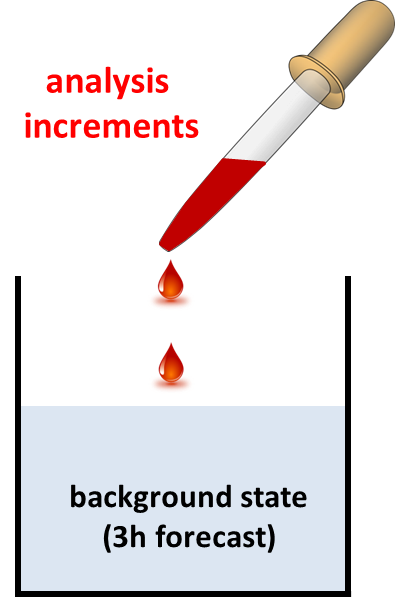
\includegraphics[width=0.30\textwidth]{analysis_drips.png}
 \caption{\textbf{I}ncremental \textbf{A}nalysis \textbf{U}pdate. Analysis increments are added to the background state (FG) in small drips over 
some time interval rather than in one go. Currently, increments for \texttt{U}, \texttt{V}, \texttt{P}, \texttt{T}, \texttt{QV} are treated in 
this way.}\label{fig_ana_drips}
\end{figure}

Mathematically speaking, during forward integration the model is forced with appropriately weighted analysis increments:
\begin{align}
 \frac{\mathrm{d} \mathbf{x}}{\mathrm{d} t} = A\mathbf{x} + g(t)\Delta\mathbf{x}^{A}\qquad \text{, with}\quad \int g(t)\, \mathrm{d}t = 1
\end{align}
$\mathbf{x}$ is the discrete model state, $A$ is a matrix representing the (non)-linear dynamics of the system and $g(t)$ is a weighting 
function, which is non-zero over some time-interval $\Delta t$.

This drip by drip incorporation acts as a low pass filter in frequency domain on the analysis increments such that 
small scale unbalanced modes are effectively filtered (see \cite{Bloom96}). The filter characteristic depends on the weighting function 
$g(t)$. It should be noted that IAU only filters the increments and not the backgound state, such that regions where analysis increments are 
zero remain unaffected. This method is currently applied to the prognostic atmospheric fields $\pi$, $\rho$, $v_{n}$, $q_{v}$, based on 
analysis increments provided for $u$, $v$, $p$, $t$ and $q_{v}$. $\pi$ denotes the Exner pressure.

The method sounds incredibly simple, however there are a few technical aspects to be taken care of when implementing this into an operational 
system: Figure \ref{fig_IAU_scheme} shows how the IAU-method is implemented in ICON for a $3\,\mathrm{h}$ assimilation run starting at midnight. 
Analysis increments are applied over a $3\,\mathrm{h}$ time window, centered at the actual model start time. As indicated by the blue line, constant 
weights are used:
\begin{align}
 g(t) = \frac{\Delta t}{T}\qquad \text{, for } -T/2 < t < T/2
\end{align}
$T$ is the window width and $\Delta t$ is the fast physics time step. The key point in terms of technical implementation is that the model 
must be started $90$ minutes prior to the actual starting time of the assimilation run. The model is started from the 22:30 UTC first guess. 
The analysis increments for \texttt{U}, \texttt{V}, \texttt{P}, \texttt{T}, \texttt{QV}, whose validity time is 00:00 UTC are added over 
$3$ hours until at 1:30 the free forecast starts. Then, two first guess data sets are written into the database. One at 1:30 UTC, which will 
be used for starting the next $3\,\mathrm{h}$ assimilation run, and a second one at 3:00 UTC, which serves as input for the assimilation system 
itself. Thus in general, using the IAU method requires some care in terms of reading and writing the right fields at the right times.
\begin{figure}[hbt]
 \centering
 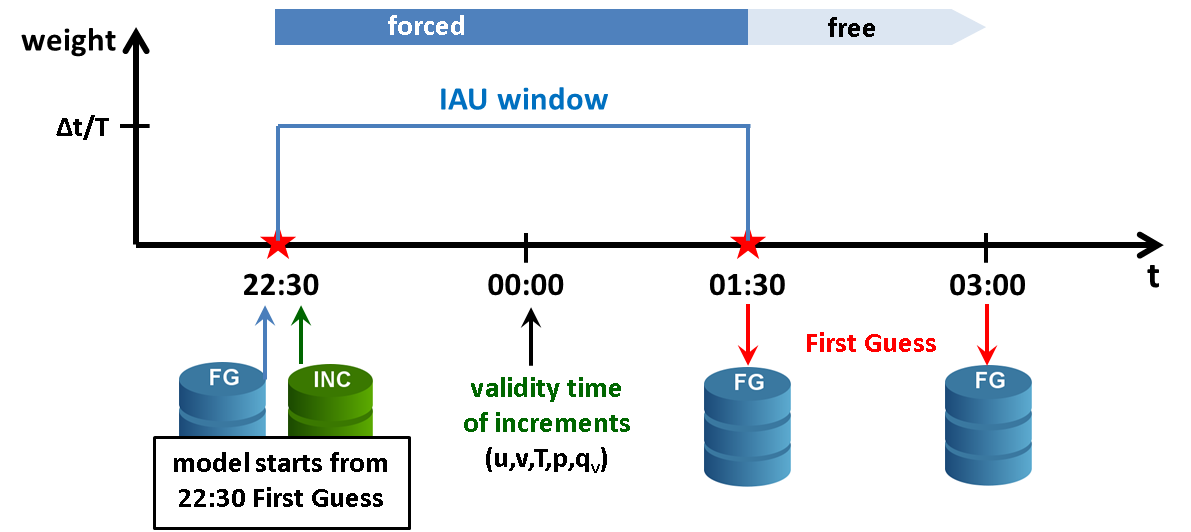
\includegraphics[width=1.0\textwidth]{IAU_scheme_2.png}
 \caption{Time line for an ICON assimilation run starting at 00:00 UTC.}\label{fig_IAU_scheme}
\end{figure}

This method is not restricted to atmospheric fields, but also applicated to
assimilated soil and surface fields, specifically soil moisture
\texttt{W\_SO}, and snow quantities \texttt{H\_SNOW} and \texttt{FRESHSNW}.

% --------------------------------------------------------------------------------

% --------------------------------------------------------------------------------
\chapter[Global output fields: Forecast runs]{Global output fields:\\ Forecast runs}

\svnInfo $Id$

ICON output fields are exclusively available in GRIB2 format (\textbf{GRI}dded \textbf{B}inary Edition \textbf{2}), with the exception of 
meteogram data (NetCDF). GRIB is a bit-oriented data storage format which was developed by WMO to facilitate the exchange of large volumes of 
gridded data between weather prediction centres. For decoding and encoding GRIB2 messages, the DWD in general and ICON in particular 
makes use of the ECMWF GRIB API. The current operational version at DWD is $1.12.3$.
 
In GRIB2, a product (i.e.\ a variable/field) is identified by a set of three parameters
% variable is uniquely defined by the following set of metadata:
\begin{itemize}
 \item \emph{Discipline} (see GRIB2 code table 0.0)
 \item \emph{ParameterCategory} (see GRIB2 code table 4.1)
 \item \emph{ParameterNumber} (see GRIB2 code table 4.2), 
\end{itemize}
augmented by a large number of additional metadata in order to uniquely describe the nature of the data. Noteworthy examples 
of additional metadata are 
\begin{itemize}
  \item \emph{typeOfFirstfixedSurface} and \emph{typeOfSecondFixedSurface} (see GRIB2 code table 4.5)
  \item \emph{typeOfStatisticalProcessing}, former known as \emph{stepType} (instant, accum, avg, max, min, diff, rms, sd, cov, \dots): describes 
        the statistical process used to calculate the field
 \end{itemize}
just to name a few.

A documentation of the official WMO GRIB2 code tables can be found here: 

\begin{minipage}{\textwidth}
\url{http://www.wmo.int/pages/prog/www/WMOCodes/WMO306_vI2/LatestVERSION/WMO306_vI2_GRIB2_CodeFlag_en.pdf}
\end{minipage}

In the following, \emph{typeOfFirstFixedSurface} and \emph{typeOfSecondFixedSurface} will be abbreviated by \emph{Lev-Typ~1/2}.



% --------------------------------------------------------------------------------
\section{Deprecated output fields}
% --------------------------------------------------------------------------------

With the launch of ICON, the following former GME output fields are no longer available:

\begin{itemize}
 \item \textbf{BAS\_CON} [\textendash]: Level index of convective cloud base. Instead, \textbf{HBAS\_CON} [m] should be used.
 \item \textbf{TOP\_CON} [\textendash]: Level index of convective cloud top. Instead, \textbf{HTOP\_CON} [m] should be used.
 \item \textbf{W\_G1}, \textbf{W\_G2}  [mm H2O]: Soil water content in upper layer ($0$ to $10\,\mathrm{cm}$) and middle layer ($10$ to $100\,\mathrm{cm}$), respectively. 
                                                 If needed, these fields can be derived from \textbf{W\_SO}.
 \item \textbf{FIS} [$\mathrm{m^{2}\,s^{-1}}$]: Surface Geopotential. Instead, \textbf{HSURF} $[\mathrm{m}]$ should be used (see Section \ref{sec_newout}).
 \item \textbf{O3} [$\mathrm{kg/kg}$], \textbf{TO3} [$\mathrm{Dobson}$]: Ozone mixing ratio and corresponding total ozone concentration. No longer available; no substitution
\end{itemize}


% --------------------------------------------------------------------------------
\section{New output fields}\label{sec_newout}
% --------------------------------------------------------------------------------

Table \ref{table_newout} contains a list of new output fields that became available with the launch of ICON (compared to GME). A more thorough description of these 
fields is provided in Section \ref{sec_outfields}.

\begin{longtable}{p{2.5cm}p{1.8cm}p{10.0cm}}
 \caption{Newly available output fields}\label{table_newout}\\
  \toprule
\multicolumn{1}{c}{\textbf{ShortName}}  &  \bf{Unit}                  & \multicolumn{1}{c}{\textbf{Description}}\\
\midrule
\endfirsthead
\caption[]{\emph{continued}}\\
\midrule
\endhead
\hline \multicolumn{3}{r}{\textit{Continued on next page}} \\
\endfoot
\endlastfoot
\midrule
\multicolumn{3}{c}{\textbf{Atmosphere}}\\
\midrule
\textbf{DEN}                            &  $\mathrm{kg\,m^{-3}}$      &  density of moist air (3D field) \\
\textbf{TKE}                            &  $\mathrm{m^{2}\,s^{-2}}$   &  Turbulent kinetic energy (3D field) \\
\textbf{DTKE\_CON}                      &  $\mathrm{m^{2}\,s^{-3}}$   &  Buoyancy-production of TKE due to sub grid scale convection (3D field) \\
\textbf{W}                              &  $\mathrm{m\,s^{-1}}$       &  vertical velocity in height coordinates $w=\frac{\mathrm{d}z}{\mathrm{d}t}$ (3D field)\\
\textbf{P}                              &  $\mathrm{Pa}$              &  pressure (3D field)\\
\midrule
\multicolumn{3}{c}{\textbf{Surface}}\\
\midrule
\textbf{CAPE\_CON}                      &  $\mathrm{J\,kg^{-1}}$      &  Convective available potential energy (2D field) \\
\textbf{QV\_2M}                         &  $\mathrm{kg\, kg^{-1}}$    &  Specific humidity at 2m above ground (2D field) \\
\textbf{RELHUM\_2M}                     &  $\mathrm{\%}$              &  Relative humidity at 2m above ground (2D field) \\
\textbf{SOBS\_RAD}                      &  $\mathrm{W\,m^{-2}}$       &  Net short-wave radiation flux at surface (instantaneous) \\
\textbf{THBS\_RAD}                      &  $\mathrm{W\,m^{-2}}$       &  Net long-wave radiation flux at surface (instantaneous) \\
\midrule
\multicolumn{3}{c}{\textbf{Lake}}\\
\midrule
\textbf{C\_T\_LK}                       &  $1$                        &  Shape factor with respect to the temperature profile in the thermocline (2D field)\\
\textbf{H\_ML\_LK}                      &  $\mathrm{m}$               &  Mixed-layer depth (2D field)\\
\textbf{T\_BOT\_LK}                     &  $\mathrm{K}$               &  Temperature at the water-bottom sediment interface (2D field)\\
\textbf{T\_MNW\_LK}                     &  $\mathrm{K}$               &  Mean temperature of the water column (2D field)\\
\textbf{T\_WML\_LK}                     &  $\mathrm{K}$               &  Mixed-layer temperature (2D field)\\
\midrule
\multicolumn{3}{c}{\textbf{Geometry}}\\
\midrule
\textbf{HSURF}                          &  $\mathrm{m}$               &  Geometric Height of the earths surface above sea level (2D field) \\
\textbf{HHL}                            &  $\mathrm{m}$               &  Geometric Height of model half levels above sea level (3D field) \\
\textbf{CLON,CLAT}                      &  $\mathrm{deg}$             &  Geographical longitude/latitude of native grid triangle cell center \\
\textbf{ELON,ELAT}                      &  $\mathrm{deg}$             &  Geographical longitude/latitude of native grid triangle edge midpoint \\
\textbf{VLON,VLAT}                      &  $\mathrm{deg}$             &  Geographical longitude/latitude of native grid triangle vertex \\
  \bottomrule
\end{longtable}



% --------------------------------------------------------------------------------
\section{Available output fields}\label{sec_outfields}
% --------------------------------------------------------------------------------

ICON forecasts are performed multiple times a day with varying forecast times. An overview of the various forecasts, including its  
forecast time and output intervals is provided in Figure \ref{fig:forecast_length}.
\begin{figure}[hbt]
 \centering
 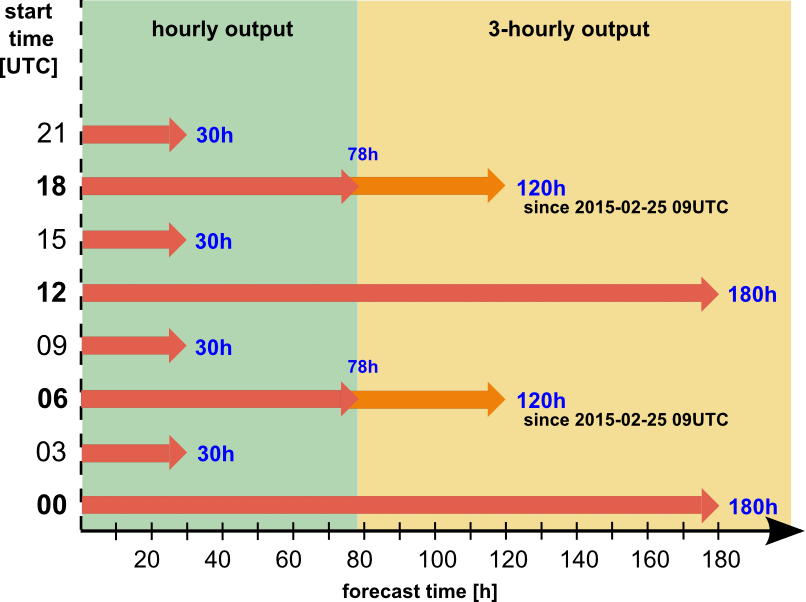
\includegraphics[width=0.90\textwidth]{forecast_length.png}
 \caption{Time span covered by the various ICON forecasts. An ICON forecast run is launched every three hours.}\label{fig:forecast_length}
\end{figure}

Main forecasts are performed $4$ times a day at $0,\, 6,\, 12,\, 18$ UTC, covering a forecast time span of $180\,\mathrm{h}$ for the 
$0$ und $12$ UTC runs and $120\,\mathrm{h}$ for the $6$ und $18$ UTC runs. Prior to 2015-02-25 the 6 and 18 UTC runs were restricted 
to $78\,\mathrm{h}$. In preparation for the replacement of COSMO-EU by a high resolution ICON nest, additional short forecasts are 
performed at 3, 9, 15 and 21UTC. These will provide boundary data for the high resolution COSMO-DE runs, once COSMO-EU has been switched off. 
The forecast time covered by these runs is limited to $30\,\mathrm{h}$. 

All time-dependent output fields are available hourly up to
$VV=78\,\mathrm{h}$ and 3-hourly for larger forecast
times\footnotemark[2].
%
Please note that for ICON fields the time unit is minutes rather than
hours, and thus differs from GME (hours).

Output is available on two distinct horizontal grids: 
\begin{itemize}
  \item The native triangular grid with an average resolution of $13\,\mathrm{km}$, and
  \item a regular latitude-longitude grid with a resolution of $\Delta \lambda = \Delta \Phi=0.25^{\circ}$. 
\end{itemize}
On the native grid most output fields are defined on triangle cell
(circum-)centers, except for \texttt{VN}, which is defined on cell
edges. On the lat-lon grid, all fields are defined on cell centers.
%
A single 2D GRIB2 field on the native and regular lat-lon grid
contains $2949120$ and $1036800$ grid points, respectively.



For details regarding the available fields, please see the tables below. Note that the vertical rules in the leftmost column indicate whether the field is 
available on the native grid ($\,$\markRed$\,$), on the lat-lon grid($\,$\markBlue$\,$), or on both grids($\,$\markRed\markBlue$\,$). 

For details regarding the algorithm for interpolation onto the lat-lon
grid, see
Section~\ref{section:technical_details_of_the_horizontal_interpolation}.

\footnotetext[2]{An exception here are the lat-lon output fields \texttt{U\_10M} and \texttt{V\_10M}, which are available hourly throughout the forecast. 
This is because \texttt{U\_10M} and \texttt{V\_10M} are needed as input by the wave models.}


% --------------------------------------------------------------------------------
\subsection{Time-constant (external parameter) fields}
% --------------------------------------------------------------------------------

Table \ref{table_constdb} provides an overview of the available time invariant fields. They are available from the database category 
\texttt{CAT\_NAME=\$model\_\tblu{const}\_\tblu{an}\_\$suite}. As mentioned in Section \ref{section:extpar}, \texttt{HSURF}, 
\texttt{FR\_LAND}, \texttt{FR\_LAKE} and \texttt{Z0} are modified by ICON. Thus, the latter should not be taken from the \emph{const\_an} 
database categorie, unless you definitely know what you are doing. For convenience, the modified invariant fields (and some more) 
are stored in the \emph{forecast} database categories for step $s[h]=0$ (\texttt{CAT\_NAME=\$model\_\$run\_\tblu{fc}\_\$suite}). Table 
\ref{table_init_output} provides a list of all fields which are exclusively written for $s[h]=0$.

See Section \ref{sec_skycat} for more details on the database categories and Section \ref{sec_example} for sample retrievals.
 

%All except for \texttt{HHL}, \texttt{ELON}, \texttt{ELAT}, 
%\texttt{VLON}, \texttt{VLAT} are available from the database category \texttt{CAT\_NAME=\$model\_\tblu{const}\_\tblu{an}\_\$suite}. However, since  
%\texttt{HSURF}, \texttt{FR\_LAND}, \texttt{FR\_LAKE} and \texttt{Z0} are modified by ICON, they should be taken as well as \texttt{HHL} from 
%\emph{forecast} database categories for step $s[h]=0$ (\texttt{CAT\_NAME=\$model\_\$run\_\tblu{fc}\_\$suite}). See Section 
%\ref{sec_skycat} for more details on the database categories and Section \ref{sec_example} for sample retrievals.


\begin{longtable}{@{}p{0.30cm}@{\hskip 0.05in}p{2.0cm}p{5.0cm}p{0.7cm}p{0.7cm}p{0.7cm}p{1.4cm}p{1cm}p{1cm}}
 \caption{Time-constant fields (\texttt{CAT\_NAME=\$model\_\tblu{const}\_\tblu{an}\_\$suite})}\label{table_constdb}\\
  \toprule
&\multicolumn{1}{c}{\begin{sideways}\textbf{ShortName}\end{sideways}}  &  \multicolumn{1}{c}{\rb{\textbf{Description}}}  & \begin{sideways}\textbf{Discipline}\end{sideways} & \begin{sideways}\bf{Category}\end{sideways} & \begin{sideways}\bf{Number}\end{sideways}  & \begin{sideways}\bf{Lev-Typ 1/2}\end{sideways}  & \begin{sideways}\bf{stepType}\end{sideways} &\begin{sideways}\bf{Unit}\end{sideways}\\
\midrule
\endfirsthead
\caption[]{\emph{continued}}\\
\midrule
\endhead
\hline \multicolumn{8}{r}{\textit{Continued on next page}} \\
\endfoot
\endlastfoot
\multicolumn{8}{c}{\textbf{Date/Time} (YYYY-MM-DDThh) \textbf{D=0001-01-01T00}}\\
\midrule
\groups[tri][]   & HSURF                         &  Geometric height of the earths surface above msl                                       &               0                                   &                       3                     &                    6                       &                 1/101                           &                      inst                   &        $\mathrm{m}$   \\ 
\groups[tri][]   & CLAT                          &  Geographical latitude of native grid triangle cell center                              &               0                                   &                     191                     &                    1                       &                 1/--                            &                      inst                   &        $\mathrm{Deg.\, N}$   \\
\groups[tri][]   & CLON                          &  Geographical longitude of native grid triangle cell center                             &               0                                   &                     191                     &                    2                       &                 1/--                            &                      inst                   &        $\mathrm{Deg.\, E}$   \\
\groups[tri][]   & FOR\_E                        &  Fraction of evergreen forest (possible range [$0,1$])                                  &               2                                   &                       0                     &                   29                       &                 1/--                            &                      inst                   &        $1$ \\
\groups[tri][]   & FOR\_D                        &  Fraction of deciduous forest (possible range [$0,1$])                                  &               2                                   &                       0                     &                   30                       &                 1/--                            &                      inst                   &        $1$ \\
\groups[tri][]   & FR\_LAND                      &  Land fraction (possible range [$0,1$])                                                 &               2                                   &                       0                     &                    0                       &                 1/--                            &                      inst                   &        $1$ \\
\groups[tri][]   & FR\_LAKE                      &  Fresh water lake fraction (possible range [$0,1$])                                     &               1                                   &                       2                     &                    2                       &                 1/--                            &                      inst                   &        $1$ \\
\groups[tri][]   & FR\_LUC                       &  Land use class fraction (possible range [$0,1$])                                       &               2                                   &                       0                     &                   36                       &                 1/--                            &                      inst                   &        $1$ \\
\groups[tri][]   & DEPTH\_LK                     &  Lake depth                                                                             &               1                                   &                       2                     &                    0                       &                 1/162                           &                      inst                   &        $\mathrm{m}$ \\
\groups[tri][]   & ROOTDP                        &  Root depth of vegetation                                                               &               2                                   &                       0                     &                   32                       &                 1/--                            &                      inst                   &        $\mathrm{m}$ \\
\groups[tri][]   & RSMIN                         &  Minimum stomatal resistance                                                            &               2                                   &                       0                     &                   16                       &                 1/--                            &                      inst                   &        $\mathrm{s\,m^{-1}}$ \\
\groups[tri][]   & EMIS\_RAD                     &  Longwave surface emissivity                                                            &               2                                   &                       3                     &                  199                       &                 1/--                            &                      inst                   &        $1$ \\
\groups[tri][]   & SOILTYP                       &  Soil type of land fraction  (9 types $[1,\dots, 9]$)                                   &               2                                   &                       3                     &                  196                       &                 1/--                            &                      inst                   &        $1$ \\
\groups[tri][]   & SSO\_STDH                     &  Standard deviation of sub-grid scale orography                                         &               0                                   &                       3                     &                   20                       &                 1/--                            &                      inst                   &        $\mathrm{m}$ \\
\groups[tri][]   & SSO\_GAMMA                    &  Anisotropy of sub-gridscale orography                                                  &               0                                   &                       3                     &                   24                       &                 1/--                            &                      inst                   &        $1$ \\
\groups[tri][]   & SSO\_THETA                    &  Angle of sub-gridscale orography                                                       &               0                                   &                       3                     &                   21                       &                 1/--                            &                      inst                   &        $\mathrm{rad}$ \\
\groups[tri][]   & SSO\_SIGMA                    &  Slope of sub-gridscale orography                                                       &               0                                   &                       3                     &                   22                       &                 1/--                            &                      inst                   &        $1$ \\
\groups[tri][]   & LAI\_MX                       &  Leaf area index in the vegetation phase                                                &               2                                   &                       0                     &                   28                       &                 1/--                            &                      max                    &        $1$ \\
\groups[tri][]   & NDVI\_MAX                     &  Normalized differential vegetation index                                               &               2                                   &                       0                     &                   31                       &                 1/--                            &                      max                    &        $1$ \\
\groups[tri][]   & PLCOV\_MX                     &  Plant covering degree in the vegetation phase                                          &               2                                   &                       0                     &                    4                       &                 1/--                            &                      max                    &        $1$ \\
\groups[tri][]   & T\_2M\_CL                     &  Climatological $2\,\mathrm{m}$ temperature (used as lower bc.\ for soil model)         &               0                                   &                       0                     &                    0                       &               103/--                            &                      inst                   &        $\mathrm{K}$ \\
\groups[tri][]   & Z0                            &  Surface roughness length (over land)                                                   &               2                                   &                       0                     &                    1                       &                 1/--                            &                      inst                   &        $\mathrm{m}$ \\
\midrule
\multicolumn{8}{c}{\textbf{Date/Time} (YYYY-MM-DDThh) \textbf{D=1111-01-11T11}}\\
\midrule
\groups[tri][] & AER\_SS12                     &  Sea salt aerosol climatology (monthly fields)                                          &               0                                   &                      20                     &                   102                      &                 1/--                            &                      avg                    &        $\mathrm{1}$ \\
\groups[tri][] & AER\_DUST12                   &  Total soil dust aerosol climatology (monthly fields)                                   &               0                                   &                      20                     &                   102                      &                 1/--                            &                      avg                    &        $\mathrm{1}$ \\
\groups[tri][] & AER\_ORG12                    &  Organic aerosol climatology (monthly fields)                                           &               0                                   &                      20                     &                   102                      &                 1/--                            &                      avg                    &        $\mathrm{1}$ \\
\groups[tri][] & AER\_SO412                    &  Total sulfate aerosol climatology (monthly fields)                                     &               0                                   &                      20                     &                   102                      &                 1/--                            &                      avg                    &        $\mathrm{1}$ \\
\groups[tri][] & AER\_BC12                     &  Black carbon aerosol climatology (monthly fields)                                      &               0                                   &                      20                     &                   102                      &                 1/--                            &                      avg                    &        $\mathrm{1}$ \\
\groups[tri][] & ALB\_DIF12                    &  Shortwave ($0.3 - 5.0\,\mathrm{\mu m}$) albedo for diffuse radiation (monthly fields)  &               0                                   &                      19                     &                    18                      &                 1/--                            &                      avg                    &        $\mathrm{1}$ \\
\groups[tri][] & ALB\_UV12                     &  UV-visible ($0.3 - 0.7\,\mathrm{\mu m}$) albedo for diffuse radiation (monthly fields) &               0                                   &                      19                     &                   222                      &                 1/--                            &                      avg                    &        $\mathrm{1}$ \\
\groups[tri][] & ALB\_NI12                     &  Near infrared ($0.7 - 5.0\,\mathrm{\mu m}$) albedo for diffuse radiation (monthly fields) &            0                                   &                      19                     &                   223                      &                 1/--                            &                      avg                    &        $\mathrm{1}$ \\
\groups[tri][] & NDVI\_MRAT                    &  ratio of monthly mean NDVI (normalized differential vegetation index) to annual max    &               0                                   &                       0                     &                   192                      &                 1/--                            &                      avg                    &        $\mathrm{1}$ \\
  \bottomrule
\end{longtable}



% LaTeX macros that are later used to disable/enable rows in the
% tables of output fields (global/local domain):
\renewcommand{\onlyglb}[1]{#1}
\renewcommand{\onlyloc}[1]{}
%
\begin{longtable}{@{}p{0.30cm}@{\hskip 0.05in}p{2.0cm}p{5.0cm}p{0.7cm}p{0.7cm}p{0.7cm}p{1.4cm}p{1cm}p{1cm}}
 \caption{Variables exclusively available for $VV=0$ from the forecast databases (\texttt{CAT\_NAME=\$model\_\$run\_\tblu{fc}\_\$suite}, $s[h]=0$)}\label{table_init_output}\\
  \toprule
&\multicolumn{1}{c}{\begin{sideways}\textbf{ShortName}\end{sideways}}  &  \multicolumn{1}{c}{\rb{\textbf{Description}}}  & \begin{sideways}\textbf{Discipline}\end{sideways} & \begin{sideways}\bf{Category}\end{sideways} & \begin{sideways}\bf{Number}\end{sideways}  & \begin{sideways}\bf{Lev-Typ 1/2}\end{sideways}  & \begin{sideways}\bf{stepType}\end{sideways} &\begin{sideways}\bf{Unit}\end{sideways}\\
\midrule
\endfirsthead
\caption[]{\emph{continued}}\\
\midrule
\endhead
\hline \multicolumn{8}{r}{\textit{Continued on next page}} \\
\endfoot
\endlastfoot
  % --------- include table of variables
  \groups[tri][]   & CLAT                          &  Geographical latitude of native grid triangle cell center                              &               0                                   &                     191                     &                    1                       &                 1/--                            &                      inst                   &        $\mathrm{Deg.\, N}$   \\
\groups[tri][]   & CLON                          &  Geographical longitude of native grid triangle cell center                             &               0                                   &                     191                     &                    2                       &                 1/--                            &                      inst                   &        $\mathrm{Deg.\, E}$   \\
\groups[tri][]   & ELAT                          &  Geographical latitude of native grid triangle edge midpoint                            &               0                                   &                     191                     &                    1                       &                 1/--                            &                      inst                   &        $\mathrm{Deg.\, N}$   \\
\groups[tri][]   & ELON                          &  Geographical longitude of native grid triangle edge midpoint                           &               0                                   &                     191                     &                    2                       &                 1/--                            &                      inst                   &        $\mathrm{Deg.\, E}$   \\
\groups[tri][]   & VLAT                          &  Geographical latitude of native grid triangle vertex                                   &               0                                   &                     191                     &                    1                       &                 1/--                            &                      inst                   &        $\mathrm{Deg.\, N}$   \\
\groups[tri][]   & VLON                          &  Geographical longitude of native grid triangle vertex                                  &               0                                   &                     191                     &                    2                       &                 1/--                            &                      inst                   &        $\mathrm{Deg.\, E}$   \\
\groups[tri][ll] & DEPTH\_LK                     &  Lake depth                                                                             &               1                                   &                       2                     &                    0                       &                 1/162                           &                      inst                   &        $\mathrm{m}$ \\
\groups[tri][ll] & FR\_LAND                      &  Land fraction (possible range [$0,1$])                                                 &               2                                   &                       0                     &                    0                       &                 1/--                            &                      inst                   &        $1$ \\
\groups[tri][ll] & FR\_LAKE                      &  Fresh water lake fraction (possible range [$0,1$])                                     &               1                                   &                       2                     &                    2                       &                 1/--                            &                      inst                   &        $1$ \\
\groups[tri][ll] & HHL                           &  Geometric height of model half levels above msl                                        &               0                                   &                       3                     &                    6                       &                 150/101                         &                      inst                   &        $\mathrm{m}$   \\
\groups[tri][ll] & HSURF                         &  Geometric height of the earths surface above msl                                       &               0                                   &                       3                     &                    6                       &                 1/101                           &                      inst                   &        $\mathrm{m}$   \\
\groups[tri][ll] & LAI                           &  Leaf area index                                                                        &               2                                   &                       0                     &                   28                       &                 1/--                            &                      inst                   &        $1$ \\
\groups[tri][]   & NDVIRATIO                     &  ratio of current NDVI (normalized differential vegetation index) to annual max         &               2                                   &                       0                     &                  192                       &                 1/--                            &                      inst                   &        $1$ \\
\groups[tri][ll] & PLCOV                         &  Plant cover                                                                            &               2                                   &                       0                     &                    4                       &                 1/--                            &                      inst                   &        $\mathrm{\%}$ \\
\groups[tri][ll] & ROOTDP                        &  Root depth of vegetation                                                               &               2                                   &                       0                     &                   32                       &                 1/--                            &                      inst                   &        $\mathrm{m}$ \\
\groups[tri][ll] & SOILTYP                       &  Soil type of land fraction  (9 types $[1,\dots, 9]$)                                   &               2                                   &                       3                     &                  196                       &                 1/--                            &                      inst                   &        $1$ \\
  % ------------------------------------
  \bottomrule
\end{longtable}


% --------------------------------------------------------------------------------
\subsection{Multi-level fields on native hybrid vertical levels}
% --------------------------------------------------------------------------------

% LaTeX macros that are later used to disable/enable rows in the
% tables of output fields (global/local domain):
\renewcommand{\onlyglb}[1]{#1}
\renewcommand{\onlyloc}[1]{}
%
\begin{table}[H]
 \caption{Hybrid multi-level forecast ($VV>0$) and initialised analysis ($VV=0$) products}
 \begin{tabular}{@{}p{0.30cm}@{\hskip 0.05in}p{2.0cm}p{5.0cm}p{0.6cm}p{0.6cm}p{0.6cm}p{1.4cm}p{1cm}p{1cm}}
  \toprule
&\multicolumn{1}{c}{\begin{sideways}\textbf{ShortName}\end{sideways}}  &  \multicolumn{1}{c}{\rb{\textbf{Description}}}  & \begin{sideways}\textbf{Discipline}\end{sideways} & \begin{sideways}\bf{Category}\end{sideways} & \begin{sideways}\bf{Number}\end{sideways}  & \begin{sideways}\bf{Lev-Typ 1/2}\end{sideways}  & \begin{sideways}\bf{stepType}\end{sideways} &\begin{sideways}\bf{Unit}\end{sideways}\\
\midrule
  % --------- include table of variables
  % TABLE OF VV>0 MULTI-LEVEL FIELDS FROM THE FORECAST DATABASE
%
% This file contains the table data for both the GLOBAL and the EU NEST:
%
% table rows that are only part of the GLOBAL  grid output should be enclosed by         \onlyglb{ ... }
% table rows that are only part of the EU NEST grid output should be enclosed by         \onlyloc{ ... }
%
% ADDITIONAL NOTES:
%
% 1. Variables required to drive INT2LM/COSMO-DE are marked by comment "i2l",
%    see "~for1han/const/iglo/namelst.output.i2l"
%    It is used by script build_varlists.py
%
%    > For the EU nest these are the fields required for the native grid. 
% 
%    ml_varlist           = 'U',         'V',         'W',         'T',         'P',
%                           'QV',        'QC',        'QI',        'QR',        'QS',
%                           'W_I',       'T_G',       'QV_S',
%                           'T_SNOW',    'W_SNOW',    'RHO_SNOW',  'FRESHSNW',
%                           'T_SO',      'W_SO',      'H_ICE',     'T_ICE',
\svnInfo $Id$
\\[-0.5em] % without this dummy line, TikZ does not seem to get the marker position right...
%
%
          \groups[\onlyglb{tri}][         ll ] & CLC                        &  Cloud cover                                                                               &               0/6/22                      &                 150/150                         &                      inst        &             &        $\mathrm{\%}$ \\             
\onlyglb{ \groups[tri          ][            ] & DEN                        &  Density of moist air                                                                      &               0/3/10                      &                 150/150                         &                      inst        &     --      &        $\mathrm{kg\,m^{-3}}$ \\     }
          \groups[tri          ][            ] & DTKE\_CON                  &  Buoyancy-production of TKE due to sub grid scale convection                               &               0/19/219                    &                 150/--                          &                      inst        &     --      &        $\mathrm{m^{2}\,s^{-3}}$ \\   
          \groups[tri          ][            ] & DTKE\_HSH                  &  Production of TKE due to horizontal shear                                                 &               0/19/220                    &                 150/--                          &                      inst        &     --      &        $\mathrm{m^{2}\,s^{-3}}$ \\   
          \groups[tri          ][         ll ] & P                          &  Pressure                                                                                  &               0/3/0                       &                 150/150                         &                      inst        &             &        $\mathrm{Pa}$         \\     % i2l 
          \groups[tri          ][         ll ] & QC                         &  \textcolor{red}{Cloud mixing ratio}\footnotemark[3]                                       &               0/1/22                      &                 150/150                         &                      inst        &             &        $\mathrm{kg\,kg^{-1}}$ \\    % i2l
          \groups[tri          ][         ll ] & QI                         &  \textcolor{red}{Cloud ice mixing ratio}\footnotemark[3]                                   &               0/1/82                      &                 150/150                         &                      inst        &             &        $\mathrm{kg\,kg^{-1}}$ \\    % i2l
          \groups[tri          ][            ] & QR                         &  \textcolor{red}{Rain mixing ratio}\footnotemark[3]                                        &               0/1/24                      &                 150/150                         &                      inst        &     --      &        $\mathrm{kg\,kg^{-1}}$ \\    % i2l
          \groups[tri          ][            ] & QS                         &  \textcolor{red}{Snow mixing ratio}\footnotemark[3]                                        &               0/1/25                      &                 150/150                         &                      inst        &     --      &        $\mathrm{kg\,kg^{-1}}$ \\    % i2l 
          \groups[tri          ][         ll ] & QV                         &  Specific humidity                                                                         &               0/1/0                       &                 150/150                         &                      inst        &             &        $\mathrm{kg\,kg^{-1}}$ \\    % i2l
          \groups[tri          ][         ll ] & T                          &  Temperature                                                                               &               0/0/0                       &                 150/150                         &                      inst        &             &        $\mathrm{K}$          \\     % i2l 
          \groups[tri          ][         ll ] & TKE                        &  Turbulent kinetic energy                                                                  &               0/19/11                     &                 150/--                          &                      inst        &             &        $\mathrm{m^{2}\,s^{-2}}$ \\  
          \groups[tri          ][         ll ] & U                          &  Zonal wind                                                                                &               0/2/2                       &                 150/150                         &                      inst        &             &        $\mathrm{m\,s^{-1}}$   \\    % i2l
          \groups[tri          ][         ll ] & V                          &  Meridional wind                                                                           &               0/2/3                       &                 150/150                         &                      inst        &             &        $\mathrm{m\,s^{-1}}$   \\    % i2l
          \groups[tri          ][         ll ] & W                          &  Vertical wind                                                                             &               0/2/9                       &                 150/--                          &                      inst        &             &        $\mathrm{m\,s^{-1}}$   \\    % i2l


  % ------------------------------------
  \bottomrule
 \end{tabular}
\end{table}
\footnotetext[2]{for the time being, erroneously encoded as mixing ratios instead of specific quantities}



% --------------------------------------------------------------------------------
\subsection{Multi-level fields interpolated to pressure levels}
% --------------------------------------------------------------------------------

\newcommand{\pressurelevelsTriangular}{$1000$, $950$, $850$, $700$, $500$, $300$ $\mathrm{hPa}$}

\newcommand{\new}[1]{\textcolor{red}{#1}}
\newcommand{\pressurelevelsRegular}{$1000$, \new{$975$}, $950$, $925$, $900$, 
                                    $875$, $850$, \new{$825$}, $800$, 
                                    \new{$775$}, $750$, \new{$725$}, $700$, $600$, 
                                    $500$, $400$, $300$, $250$, $200$, $150$, $100$, 
                                    $70$, $50$, $30$, \new{$20$}, $10$, 
                                    \new{$7$}, $5$, \new{$3$}, 
                                    \new{$2$}, \new{$1$}, 
                                     \new{$0.3$}, \new{$0.1$} $\mathrm{hPa}$}

For regular grid output the following pressure levels are available: 
\begin{center}
\begin{minipage}{0.5\linewidth}
\pressurelevelsRegular. 
\end{minipage}
\end{center}


Newly available pressure levels (as compared to GME) are highlighted in red. 
The output fields are listed in Table~\ref{table:output_pressurelevels_regular}.
I.e.\ note that all $17$ WMO standard pressure levels are included.

\begin{table}
\renewcommand{\new}[1]{#1}
\caption{Regular grid output:
         Multi-level forecast ($VV>0$) and initialised analysis ($VV=0$) products 
         interpolated to pressure levels \pressurelevelsRegular.}
 \begin{tabular}{@{}p{0.30cm}@{\hskip 0.05in}p{2.0cm}p{5.0cm}p{0.6cm}p{0.6cm}p{0.6cm}p{1.4cm}p{1cm}p{1cm}}
  \toprule
&\multicolumn{1}{c}{\begin{sideways}\textbf{ShortName}\end{sideways}}  &  \multicolumn{1}{c}{\rb{\textbf{Description}}}  & \begin{sideways}\textbf{Discipline}\end{sideways} & \begin{sideways}\bf{Category}\end{sideways} & \begin{sideways}\bf{Number}\end{sideways}  & \begin{sideways}\bf{Lev-Typ 1/2}\end{sideways}  & \begin{sideways}\bf{stepType}\end{sideways} &\begin{sideways}\bf{Unit}\end{sideways}\\
\midrule
\groups[][ll] & FI                         &  Geopotential                                                                              &               0                                   &                     3                       &                    4                       &                 100/--                          &                      inst                   &        $\mathrm{m^{2}\,s^{-2}}$   \\
\groups[][ll] & OMEGA                      &  Vertical velocity in pressure coordinates ($\omega=\mathrm{d}p/\mathrm{d}t$)              &               0                                   &                     2                       &                    8                       &                 100/--                          &                      inst                   &        $\mathrm{Pa\,s^{-1}}$  \\
\groups[][ll] & RELHUM                     &  Relative humidity (with respect to water)                                                 &               0                                   &                     1                       &                    1                       &                 100/--                          &                      inst                   &        $\mathrm{\%}$          \\
\groups[][ll] & T                          &  Temperature                                                                               &               0                                   &                     0                       &                    0                       &                 100/--                          &                      inst                   &        $\mathrm{K}$          \\
\groups[][ll] & U                          &  Zonal wind                                                                                &               0                                   &                     2                       &                    2                       &                 100/--                          &                      inst                   &        $\mathrm{m\,s^{-1}}$   \\ 
\groups[][ll] & V                          &  Meridional wind                                                                           &               0                                   &                     2                       &                    3                       &                 100/--                          &                      inst                   &        $\mathrm{m\,s^{-1}}$   \\
  \bottomrule
 \end{tabular}
\label{table:output_pressurelevels_regular}%
\end{table}

\begin{table}
\caption{Native (triangular) grid output:
         Multi-level forecast ($VV>0$) and initialised analysis ($VV=0$) products interpolated to pressure levels \pressurelevelsTriangular.}
 \begin{tabular}{@{}p{0.30cm}@{\hskip 0.05in}p{2.0cm}p{5.0cm}p{0.6cm}p{0.6cm}p{0.6cm}p{1.4cm}p{1cm}p{1cm}}
  \toprule
&\multicolumn{1}{c}{\begin{sideways}\textbf{ShortName}\end{sideways}}  &  \multicolumn{1}{c}{\rb{\textbf{Description}}}  & \begin{sideways}\textbf{Discipline}\end{sideways} & \begin{sideways}\bf{Category}\end{sideways} & \begin{sideways}\bf{Number}\end{sideways}  & \begin{sideways}\bf{Lev-Typ 1/2}\end{sideways}  & \begin{sideways}\bf{stepType}\end{sideways} &\begin{sideways}\bf{Unit}\end{sideways}\\
\midrule
\groups[tri][] & FI                         &  Geopotential                                                                              &               0                                   &                     3                       &                    4                       &                 100/--                          &                      inst                   &        $\mathrm{m^{2}\,s^{-2}}$   \\
\groups[tri][] & RELHUM                     &  Relative humidity (with respect to water)                                                 &               0                                   &                     1                       &                    1                       &                 100/--                          &                      inst                   &        $\mathrm{\%}$          \\
\groups[tri][] & T                          &  Temperature                                                                               &               0                                   &                     0                       &                    0                       &                 100/--                          &                      inst                   &        $\mathrm{K}$          \\
\groups[tri][] & U                          &  Zonal wind                                                                                &               0                                   &                     2                       &                    2                       &                 100/--                          &                      inst                   &        $\mathrm{m\,s^{-1}}$   \\ 
\groups[tri][] & V                          &  Meridional wind                                                                           &               0                                   &                     2                       &                    3                       &                 100/--                          &                      inst                   &        $\mathrm{m\,s^{-1}}$   \\
  \bottomrule
 \end{tabular}
\label{table:output_pressurelevels_triangular}%
\end{table}

On the native (triangular) grid, output is generated for levels
\begin{center}
\begin{minipage}{0.5\linewidth}
 \pressurelevelsTriangular.
\end{minipage}
\end{center}
The output fields are listed in Table~\ref{table:output_pressurelevels_triangular}.


\newpage


% --------------------------------------------------------------------------------
\subsection{Multi-level fields interpolated to height levels}
% --------------------------------------------------------------------------------

\newcommand{\heightlevelsRegular}{$10000$, $5000$, $3000$, $2000$, $1500$, $1000$, $500$, $100$ $\mathrm{m}$}

\begin{table}[H]
\caption{Regular grid output:
         Multi-level forecast ($VV>0$) and initialised analysis ($VV=0$) products interpolated to height levels \heightlevelsRegular
         ~(above mean sea level).}
 \begin{tabular}{@{}p{0.30cm}@{\hskip 0.05in}p{2.0cm}p{5.0cm}p{0.6cm}p{0.6cm}p{0.6cm}p{1.4cm}p{1cm}p{1cm}}
  \toprule
&\multicolumn{1}{c}{\begin{sideways}\textbf{ShortName}\end{sideways}}  &  \multicolumn{1}{c}{\rb{\textbf{Description}}}  & \begin{sideways}\textbf{Discipline}\end{sideways} & \begin{sideways}\bf{Category}\end{sideways} & \begin{sideways}\bf{Number}\end{sideways}  & \begin{sideways}\bf{Lev-Typ 1/2}\end{sideways}  & \begin{sideways}\bf{stepType}\end{sideways} &\begin{sideways}\bf{Unit}\end{sideways}\\
\midrule
\groups[][ll] & U                          &  Zonal wind                                                                                &               0                                   &                     2                       &                    2                       &                 100/--                          &                      inst                   &        $\mathrm{m\,s^{-1}}$   \\ 
\groups[][ll] & V                          &  Meridional wind                                                                           &               0                                   &                     2                       &                    3                       &                 100/--                          &                      inst                   &        $\mathrm{m\,s^{-1}}$   \\
\groups[][ll] & W                          &  Vertical wind                                                                             &               0                                   &                     2                       &                    9                       &                 150/--                          &                      inst                   &        $\mathrm{m\,s^{-1}}$   \\
\groups[][ll] & T                          &  Temperature                                                                               &               0                                   &                     0                       &                    0                       &                 100/--                          &                      inst                   &        $\mathrm{K}$          \\
\groups[][ll] & P                          &  Pressure                                                                                  &               0                                   &                     3                       &                    0                       &                 150/150                         &                      inst                   &        $\mathrm{Pa}$         \\
  \bottomrule
 \end{tabular}
\label{table:output_heightlevels_regular}%
\end{table}


\newpage

% --------------------------------------------------------------------------------
\subsection{Single-level fields}
% --------------------------------------------------------------------------------

% LaTeX macros that are later used to disable/enable rows in the
% tables of output fields (global/local domain):
\renewcommand{\onlyglb}[1]{#1}
\renewcommand{\onlyloc}[1]{}
%
\begin{longtable}{@{}p{0.30cm}@{\hskip 0.05in}p{2.0cm}p{5.0cm}p{0.7cm}p{0.7cm}p{0.7cm}p{1.4cm}p{1cm}p{1cm}}
\caption[]{Single-level forecast ($VV>0$) and initialised analysis ($VV=0$) products}\\
  \toprule
&\multicolumn{1}{c}{\begin{sideways}\textbf{ShortName}\end{sideways}}  &  \multicolumn{1}{c}{\rb{\textbf{Description}}}  & \begin{sideways}\textbf{Discipline}\end{sideways} & \begin{sideways}\bf{Category}\end{sideways} & \begin{sideways}\bf{Number}\end{sideways}  & \begin{sideways}\bf{Lev-Typ 1/2}\end{sideways}  & \begin{sideways}\bf{stepType}\end{sideways} &\begin{sideways}\bf{Unit}\end{sideways}\\
\midrule
\endfirsthead
\caption[]{\emph{continued}}\\
\midrule
\endhead
\hline \multicolumn{8}{r}{\textit{Continued on next page}} \\
\endfoot
\endlastfoot
  % --------- include table of variables
  % TABLE OF VV>0 MULTI-LEVEL FIELDS FROM THE FORECAST DATABASE
%
% This file contains the table data for both the GLOBAL and the EU NEST:
%
% table rows that are only part of the GLOBAL  grid output should be enclosed by         \onlyglb{ ... }
% table rows that are only part of the EU NEST grid output should be enclosed by         \onlyloc{ ... }
%
% ADDITIONAL NOTES:
%
% 1. Variables required to drive INT2LM/COSMO-DE are marked by comment "i2l",
%    see "~for1han/const/iglo/namelst.output.i2l"
%    It is used by script build_varlists.py
%
%    > For the EU nest these are the fields required for the native grid. 
% 
%    ml_varlist           = 'U',         'V',         'W',         'T',         'P',
%                           'QV',        'QC',        'QI',        'QR',        'QS',
%                           'W_I',       'T_G',       'QV_S',
%                           'T_SNOW',    'W_SNOW',    'RHO_SNOW',  'FRESHSNW',
%                           'T_SO',      'W_SO',      'H_ICE',     'T_ICE',
%
%
\svnInfo $Id$
\\[-0.5em] % without this dummy line, TikZ does not seem to get the marker position right...
%
%
           \groups[\onlyglb{tri}][         ll ] & ALB\_RAD                       &  Shortwave broadband albedo for diffuse radiation                                      &               0                                   &                    19                       &                     1                      &                 1/--                            &                      inst                   &        $\mathrm{\%}$    \\            
           \groups[\onlyglb{tri}][         ll ] & ALHFL\_S                       &  Latent heat net flux at surface (average since model start)                           &               0                                   &                     0                       &                    10                      &                 1/--                            &                      avg                    &        $\mathrm{W\,m^{-2}}$  \\
           \groups[             ][         ll ] & APAB\_S                        &  Photosynthetically active radiation flux at surface (average since model start)       &               0                                   &                     4                       &                    10                      &                 1/--                            &                      avg                    &        $\mathrm{W\,m^{-2}}$    \\    
           \groups[\onlyglb{tri}][         ll ] & ASHFL\_S                       &  Sensible heat net flux at surface (average since model start)                         &               0                                   &                     0                       &                    11                      &                 1/--                            &                      avg                    &        $\mathrm{W\,m^{-2}}$  \\
           \groups[\onlyglb{tri}][         ll ] & ASOB\_S                        &  Net short-wave radiation flux at surface (average since model start)                  &               0                                   &                     4                       &                     9                      &                 1/--                            &                      avg                    &        $\mathrm{W\,m^{-2}}$    \\    
           \groups[\onlyglb{tri}][         ll ] & ASOB\_T                        &  Net short-wave radiation flux at TOA (average since model start)                      &               0                                   &                     4                       &                     9                      &                 8/--                            &                      avg                    &        $\mathrm{W\,m^{-2}}$    \\    
           \groups[\onlyglb{tri}][         ll ] & ASWDIFD\_S                     &  Surface down solar diffuse radiation (average since model start)                      &               0                                   &                     4                       &                   199                      &                 1/--                            &                      avg                    &        $\mathrm{W\,m^{-2}}$  \\      
           \groups[\onlyglb{tri}][         ll ] & ASWDIFU\_S                     &  Surface up solar diffuse radiation (average since model start)                        &               0                                   &                     4                       &                     8                      &                 1/--                            &                      avg                    &        $\mathrm{W\,m^{-2}}$  \\      
           \groups[\onlyglb{tri}][         ll ] & ASWDIR\_S                      &  Surface down solar direct radiation (average since model start)                       &               0                                   &                     4                       &                   198                      &                 1/--                            &                      avg                    &        $\mathrm{W\,m^{-2}}$  \\      
           \groups[\onlyglb{tri}][         ll ] & ATHB\_S                        &  Net long-wave radiation flux at surface (average since model start)                   &               0                                   &                     5                       &                     5                      &                 1/--                            &                      avg                    &        $\mathrm{W\,m^{-2}}$    \\    
           \groups[\onlyglb{tri}][         ll ] & ATHB\_T                        &  Net long-wave radiation flux at TOA (average since model start)                       &               0                                   &                     5                       &                     5                      &                 8/--                            &                      avg                    &        $\mathrm{W\,m^{-2}}$    \\    
           \groups[\onlyglb{tri}][         ll ] & AUMFL\_S                       &  U-momentum flux at surface $\overline{u^{\prime}w^{\prime}}^{1/2}$ (average since model start)&       0                                   &                     2                       &                    17                      &                 1/--                            &                      avg                    &        $\mathrm{m}$  \\ 
           \groups[\onlyglb{tri}][         ll ] & AVMFL\_S                       &  V-momentum flux at surface $\overline{v^{\prime}w^{\prime}}^{1/2}$ (average since model start)&       0                                   &                     2                       &                    18                      &                 1/--                            &                      avg                    &        $\mathrm{m}$  \\ 
           \groups[\onlyglb{tri}][\onlyloc{ll}] & CAPE\_CON                      &  Convective available potential energy                                                 &               0                                   &                     7                       &                     6                      &                 1/--                            &                      inst                   &        $\mathrm{J\,kg^{-1}}$  \\  
           \groups[\onlyglb{tri}][         ll ] & CLCH                           &  High level clouds                                                                     &               0                                   &                     6                       &                    22                      &                 100/100                         &                      inst                   &        $\mathrm{\%}$          \\    
           \groups[\onlyglb{tri}][         ll ] & CLCM                           &  Mid level clouds                                                                      &               0                                   &                     6                       &                    22                      &                 100/100                         &                      inst                   &        $\mathrm{\%}$          \\    
           \groups[\onlyglb{tri}][         ll ] & CLCL                           &  Low level clouds                                                                      &               0                                   &                     6                       &                    22                      &                 100/1                           &                      inst                   &        $\mathrm{\%}$          \\    
           \groups[\onlyglb{tri}][         ll ] & CLCT                           &  Total cloud cover                                                                     &               0                                   &                     6                       &                     1                      &                 1/--                            &                      inst                   &        $\mathrm{\%}$          \\    
           \groups[             ][         ll ] & CLCT\_MOD                      &  Modified total cloud cover for media                                                  &               0                                   &                     6                       &                   199                      &                 1/--                            &                      inst                   &        $1$                    \\     
           \groups[             ][         ll ] & CLDEPTH                        &  Modified cloud depth for media                                                        &               0                                   &                     6                       &                   198                      &                 1/--                            &                      inst                   &        $1$                    \\     
           \groups[         tri ][            ] & FRESHSNW                       &  Fresh snow factor (weighting function for albedo indicating freshness of snow)        &               0                                   &                     1                       &                   203                      &                 1/--                            &                      inst                   &        $1$  \\                       % i2l
           \groups[         tri ][            ] & FR\_ICE                        &  Sea/lake ice cover  (possible range: $[0,1]$)                                         &              10                                   &                     2                       &                     0                      &                 1/--                            &                      inst                   &        $1$  \\
           \groups[\onlyglb{tri}][         ll ] & HBAS\_CON                      &  Height of convective cloud base above msl                                             &               0                                   &                     6                       &                    26                      &                 2/101                           &                      inst                   &        $\mathrm{m}$  \\              
           \groups[         tri ][         ll ] & H\_ICE                         &  Sea/Lake ice thickness (Max: $3\,\mathrm{m}$)                                         &              10                                   &                     2                       &                     1                      &                 1/--                            &                      inst                   &        $\mathrm{m}$  \\             % i2l
           \groups[\onlyglb{tri}][         ll ] & H\_SNOW                        &  Snow depth                                                                            &               0                                   &                     1                       &                    11                      &                 1/--                            &                      inst                   &        $\mathrm{m}$  \\              
           \groups[\onlyglb{tri}][         ll ] & HTOP\_CON                      &  Height of convective cloud top above msl                                              &               0                                   &                     6                       &                    27                      &                 3/101                           &                      inst                   &        $\mathrm{m}$  \\              
           \groups[\onlyglb{tri}][         ll ] & HTOP\_DC                       &  Height of top of dry convection above msl                                             &               0                                   &                     6                       &                   196                      &                 3/101                           &                      inst                   &        $\mathrm{m}$  \\              
           \groups[\onlyglb{tri}][         ll ] & HZEROCL                        &  Height of 0 degree Celsius isotherm above msl                                         &               0                                   &                     3                       &                     6                      &                 4/101                           &                      inst                   &        $\mathrm{m}$  \\              
           \groups[             ][         ll ] & PMSL                           &  Surface pressure reduced to msl                                                       &               0                                   &                     3                       &                     1                      &                 101/--                          &                      inst                   &        $\mathrm{Pa}$   \\
           \groups[\onlyglb{tri}][         ll ] & PS                             &  Surface pressure (not reduced)                                                        &               0                                   &                     3                       &                    0                       &                 1/--                            &                      inst                   &        $\mathrm{Pa}$   \\            
           \groups[             ][         ll ] & QV\_2M                         &  Specific humidity at 2m above ground                                                  &               0                                   &                     1                       &                     0                      &               103/--                            &                      inst                   &        $\mathrm{kg\,kg^{-1}}$ \\
           \groups[         tri ][         ll ] & QV\_S                          &  Surface specific humidity                                                             &               0                                   &                     1                       &                    0                       &                 1/--                            &                      inst                   &        $\mathrm{kg\,kg^{-1}}$    \\ % i2l 
           \groups[\onlyglb{tri}][         ll ] & RAIN\_CON\onlyglb{\footnotemark[4]} &  Convective rain (accumulated since model start)                                  &               0                                   &                     1                       &                    76                      &                 1/--                            &                      accu                   &        $\mathrm{kg\,m^{-2}}$    \\   
           \groups[\onlyglb{tri}][         ll ] & RAIN\_GSP\onlyglb{\footnotemark[4]} &  Large scale rain (accumulated since model start)                                 &               0                                   &                     1                       &                    77                      &                 1/--                            &                      accu                   &        $\mathrm{kg\,m^{-2}}$    \\   
           \groups[             ][         ll ] & RELHUM\_2M                     &  Relative humidity at 2m above ground                                                  &               0                                   &                     1                       &                     1                      &               103/--                            &                      inst                   &        $\mathrm{\%}$     \\          
           \groups[         tri ][         ll ] & RHO\_SNOW                      &  Snow density                                                                          &               0                                   &                     1                       &                    61                      &                 1/--                            &                      inst                   &        $\mathrm{kg\,m^{-3}}$  \\     % i2l
 \onlyglb{ \groups[         tri ][            ] & RSTOM                          &  Stomatal resistance                                                                   &               2                                   &                     0                       &                   195                      &                 1/--                            &                      inst                   &        $\mathrm{s\,m^{-1}}$  \\     }
           \groups[\onlyglb{tri}][         ll ] & RUNOFF\_G                      &  Soil water runoff (accumulated since model start)                                     &               2                                   &                     0                       &                     5                      &                 106/--                          &                      accu                   &        $\mathrm{kg\,m^{-2}}$  \\                                    
           \groups[\onlyglb{tri}][         ll ] & RUNOFF\_S                      &  Surface water runoff (accumulated since model start)                                  &               2                                   &                     0                       &                     5                      &                 106/--                          &                      accu                   &        $\mathrm{kg\,m^{-2}}$  \\     
           \groups[\onlyglb{tri}][         ll ] & SNOW\_CON\onlyglb{\footnotemark[4]} &  Convective snowfall water equivalent (accumulated since model start)             &               0                                   &                     1                       &                    55                      &                 1/--                            &                      accu                   &        $\mathrm{kg\,m^{-2}}$    \\   
           \groups[\onlyglb{tri}][         ll ] & SNOW\_GSP\onlyglb{\footnotemark[4]} &  Large snowfall water equivalent (accumulated since model start)                  &               0                                   &                     1                       &                    56                      &                 1/--                            &                      accu                   &        $\mathrm{kg\,m^{-2}}$    \\   
 \onlyloc{ \groups[             ][         ll ] & SNOWLMT\footnotemark[5]        &  Height of snowfall limit above MSL                                                    &               0                                   &                     1                       &                   204                      &                 4/101                           &                      inst                   &        $\mathrm{m}$    \\   }
 \onlyglb{ \groups[             ][         ll ] & SOBS\_RAD                      &  Net short-wave radiation flux at surface (instantaneous)                              &               0                                   &                     4                       &                     9                      &                 1/--                            &                      inst                   &        $\mathrm{W\,m^{-2}}$    \\    }
           \groups[\onlyglb{tri}][         ll ] & T\_2M                          &  Temperature at 2m above ground                                                        &               0                                   &                     0                       &                     0                      &               103/--                            &                      inst                   &        $\mathrm{K}$          \\      
           \groups[\onlyglb{tri}][         ll ] & TCH                            &  Turbulent transfer coefficient for heat and moisture (surface)                        &               0                                   &                     0                       &                    19                      &                 1/--                            &                      inst                   &        $1$    \\ 
           \groups[\onlyglb{tri}][         ll ] & TCM                            &  Turbulent transfer coefficient for momentum (surface)                                 &               0                                   &                     2                       &                    29                      &                 1/--                            &                      inst                   &        $1$    \\ 
           \groups[\onlyglb{tri}][         ll ] & TD\_2M                         &  Dew point temperature at 2m above ground                                              &               0                                   &                     0                       &                     6                      &               103/--                            &                      inst                   &        $\mathrm{K}$          \\      
           \groups[         tri ][         ll ] & T\_G                           &  Ground temperature (temperature at sfc-atm interface)                                 &               0                                   &                     0                       &                    0                       &                 1/--                            &                      inst                   &        $\mathrm{K}$    \\           % i2l
 \onlyglb{ \groups[             ][         ll ] & THBS\_RAD                      &  Net long-wave radiation flux at surface (instantaneous)                               &               0                                   &                     5                       &                     5                      &                 1/--                            &                      inst                   &        $\mathrm{W\,m^{-2}}$    \\    }
           \groups[         tri ][         ll ] & T\_ICE                         &  Sea/Lake ice temperature (at ice-atm interface)                                       &              10                                   &                     2                       &                     8                      &                 1/--                            &                      inst                   &        $\mathrm{K}$  \\             % i2l 
           \groups[\onlyglb{tri}][         ll ] & TMAX\_2M                       &  Maximum temperature at 2m above ground                                                &               0                                   &                     0                       &                     0                      &               103/--                            &                      max                    &        $\mathrm{K}$          \\     
           \groups[\onlyglb{tri}][         ll ] & TMIN\_2M                       &  Minimum temperature at 2m above ground                                                &               0                                   &                     0                       &                     0                      &               103/--                            &                      min                    &        $\mathrm{K}$          \\     
           \groups[\onlyglb{tri}][         ll ] & TOT\_PREC\onlyglb{\footnotemark[4]} &  Total precipitation (accumulated since model start)                              &               0                                   &                     1                       &                    52                      &                 1/--                            &                      accu                   &        $\mathrm{kg\,m^{-2}}$  \\     
           \groups[\onlyglb{tri}][         ll ] & TQC                            &  Column integrated cloud water (grid scale)                                            &               0                                   &                     1                       &                    69                      &                 1/--                            &                      inst                   &        $\mathrm{kg\,m^{-2}}$  \\    
 \onlyglb{ \groups[         tri ][         ll ] & TQC\_DIA                       &  Total column integrated cloud water (including sub-grid-scale contribution)           &               0                                   &                     1                       &                   215                      &                 1/--                            &                      inst                   &        $\mathrm{kg\,m^{-2}}$  \\    }
           \groups[\onlyglb{tri}][         ll ] & TQI                            &  Column integrated cloud ice (grid scale)                                              &               0                                   &                     1                       &                    70                      &                 1/--                            &                      inst                   &        $\mathrm{kg\,m^{-2}}$  \\    
 \onlyglb{ \groups[         tri ][         ll ] & TQI\_DIA                       &  Total column integrated cloud ice (including sub-grid-scale contribution)             &               0                                   &                     1                       &                   216                      &                 1/--                            &                      inst                   &        $\mathrm{kg\,m^{-2}}$  \\    }
           \groups[\onlyglb{tri}][         ll ] & TQR                            &  Column integrated rain (grid scale)                                                   &               0                                   &                     1                       &                    45                      &                 1/--                            &                      inst                   &        $\mathrm{kg\,m^{-2}}$  \\
           \groups[\onlyglb{tri}][         ll ] & TQS                            &  Column integrated snow (grid scale)                                                   &               0                                   &                     1                       &                    46                      &                 1/--                            &                      inst                   &        $\mathrm{kg\,m^{-2}}$  \\ 
           \groups[\onlyglb{tri}][         ll ] & TQV                            &  Column integrated water vapour (grid scale)                                           &               0                                   &                     1                       &                    64                      &                 1/--                            &                      inst                   &        $\mathrm{kg\,m^{-2}}$  \\    
           \groups[\onlyglb{tri}][\onlyloc{ll}] & T\_S                           &  Temperature of the soil surface (equivalent to T\_SO(0))                              &               2                                   &                     3                       &                    18                      &                 1/--                            &                      inst                   &        $\mathrm{K}$    \\             
           \groups[         tri ][         ll ] & T\_SNOW                        &  Temperature of the snow surface                                                       &               0                                   &                     0                       &                    18                      &                 1/--                            &                      inst                   &        $\mathrm{K}$    \\            % i2l
           \groups[\onlyglb{tri}][         ll ] & U\_10M                         &  Zonal wind at 10m above ground                                                        &               0                                   &                     2                       &                     2                      &               103/--                            &                      inst                   &        $\mathrm{m\,s^{-1}}$  \\      
           \groups[\onlyglb{tri}][         ll ] & V\_10M                         &  Meridional wind at 10m above ground                                                   &               0                                   &                     2                       &                     3                      &               103/--                            &                      inst                   &        $\mathrm{m\,s^{-1}}$  \\      
           \groups[\onlyglb{tri}][         ll ] & VMAX\_10M                      &  Maximum wind at $10\,\mathrm{m}$ above ground                                         &               0                                   &                     2                       &                    22                      &               103/--                            &                      max                    &        $\mathrm{m\,s^{-1}}$   \\     
           \groups[         tri ][            ] & W\_I                           &  Plant canopy surface water                                                            &               2                                   &                     0                       &                    13                      &                 1/--                            &                      inst                   &        $\mathrm{kg\,m^{-2}}$    \\ % i2l
           \groups[         tri ][         ll ] & W\_SNOW                        &  Snow depth water equivalent                                                           &               0                                   &                     1                       &                    60                      &                 1/--                            &                      inst                   &        $\mathrm{kg\,m^{-2}}$    \\    % i2l
           \groups[\onlyglb{tri}][         ll ] & WW                             &  Weather interpretation  (WMO)                                                         &               0                                   &                    19                       &                    25                      &                 1/--                            &                      inst                   &        $1$ \\                        
           \groups[\onlyglb{tri}][         ll ] & Z0                             &  Surface roughness (above land and water)                                              &               2                                   &                     0                       &                     1                      &                 1/--                            &                      inst                   &        $\mathrm{m}$          \\      

  % ------------------------------------
  \bottomrule
\end{longtable}



\footnotetext[4]{Note that the unit which is displayed, when inspecting the GRIB2 message with \emph{grib\_dump} is $\mathrm{kg\,m^{-2}\,s^{-1}}$ 
rather than $\mathrm{kg\,m^{-2}}$. Mathematically this is wrong, however, it is in accordance with the GRIB2 standard. To get the mathematically correct 
unit for accumulated fields (\emph{typeOfStatisticalProcessing}=1), the unit displayed by \emph{grib\_dump} must be multiplied by $\mathrm{s}$.}


% --------------------------------------------------------------------------------
\subsection{Surface fields interpolated to msl}
% --------------------------------------------------------------------------------

\begin{table}[H]
\caption{Forecast ($VV>0$) and initialised analysis ($VV=0$) products interpolated to msl}
 \begin{tabular}{@{}p{0.30cm}@{\hskip 0.05in}p{2.0cm}p{5.0cm}p{0.7cm}p{0.7cm}p{0.7cm}p{1.4cm}p{1cm}p{1cm}}
  \toprule
&\multicolumn{1}{c}{\begin{sideways}\textbf{ShortName}\end{sideways}}  &  \multicolumn{1}{c}{\rb{\textbf{Description}}}  & \begin{sideways}\textbf{Discipline}\end{sideways} & \begin{sideways}\bf{Category}\end{sideways} & \begin{sideways}\bf{Number}\end{sideways}  & \begin{sideways}\bf{Lev-Typ 1/2}\end{sideways}  & \begin{sideways}\bf{stepType}\end{sideways} &\begin{sideways}\bf{Unit}\end{sideways}\\
\midrule
\groups[tri][ll] & PMSL                       &  Surface pressure reduced to msl                                                           &               0                                   &                     3                       &                    1                       &                 101/--                          &                      inst                   &        $\mathrm{Pa}$   \\
  \bottomrule
 \end{tabular}
\end{table}


\newpage

% --------------------------------------------------------------------------------
\subsection{Soil-specific multi-level fields}
% --------------------------------------------------------------------------------

\begin{longtable}{@{}p{0.30cm}@{\hskip 0.05in}p{2.0cm}p{5.0cm}p{0.6cm}p{0.6cm}p{0.6cm}p{1.4cm}p{1cm}p{1cm}}
\caption[]{Multi-level forecast ($VV>0$) and initialised analysis ($VV=0$) products of the soil model}\\
  \toprule
&\multicolumn{1}{c}{\begin{sideways}\textbf{ShortName}\end{sideways}}  &  \multicolumn{1}{c}{\rb{\textbf{Description}}}  & \begin{sideways}\textbf{Discipline}\end{sideways} & \begin{sideways}\bf{Category}\end{sideways} & \begin{sideways}\bf{Number}\end{sideways}  & \begin{sideways}\bf{Lev-Typ 1/2}\end{sideways}  & \begin{sideways}\bf{stepType}\end{sideways} &\begin{sideways}\bf{Unit}\end{sideways}\\
\midrule
%\endfirsthead
%\caption[]{\emph{continued}}\\
%\midrule
\endhead
\hline \multicolumn{8}{r}{\textit{Continued on next page}} \\
\endfoot
\endlastfoot
\groups[tri][ll] & T\_SO                          &  Soil temperature                                                                      &               2                                   &                     3                       &                    18                       &               106/--                           &                      inst                   &        $\mathrm{K}$   \\
\groups[tri][ll] & W\_SO                          &  Soil moisture integrated over individual soil layers  (ice + liquid)                  &               2                                   &                     3                       &                    20                       &               106/106                          &                      inst                   &        $\mathrm{kg\,m^{-2}}$   \\
\groups[tri][ll] & W\_SO\_ICE                     &  Soil ice content integrated over individual soil layers                               &               2                                   &                     3                       &                    22                       &               106/106                          &                      inst                   &        $\mathrm{kg\,m^{-2}}$   \\
  \bottomrule
\end{longtable}

Soil temperature is defined at the soil depths given in Table \ref{tab_soillayer} (column 2). Levels $1$ to $8$ define the full levels of the soil model. A zero gradient 
condition is assumed between levels $0$ and $1$, meaning that temperatures at the surface-atmosphere interface are set equal to the temperature at the first full level depth.
($0.5\,\mathrm{cm}$). Temperatures are prognosed for layers $1$ to $7$. At the lowermost layer (mid-level height $1458\,\mathrm{cm}$) the temperature is fixed 
to the climatological average $2\,\mathrm{m}$-temperature.

Soil moisture \texttt{W\_SO} is prognosed for layers $1$ to $6$. In the two lowermost layers \texttt{W\_SO} is filled with \texttt{W\_SO(6)} (zero gradient condition).
\begin{table}[H]
\center
\caption{Soil model: vertical distribution of levels and layers}\label{tab_soillayer}
 \begin{tabular}{>{\centering\arraybackslash}p{2.0cm}>{\centering\arraybackslash}p{2.5cm}|>{\centering\arraybackslash}p{2.5cm}>{\centering\arraybackslash}p{5.0cm}}
 \toprule
  \bf{level no.}       &  \bf{depth [cm]}        &   \bf{layer no.}        & \bf{upper/lower bounds [cm]} \\
 \midrule
         0             &     $0.0$               &                         &                                     \\
         1             &     $0.5$               &         1               &     $0.0$\, \textemdash\, $1.0$     \\
         2             &     $2.0$               &         2               &     $1.0$\, \textemdash\, $3.0$     \\
         3             &     $6.0$               &         3               &     $3.0$\, \textemdash\, $9.0$     \\
         4             &     $18.0$              &         4               &     $9.0$\, \textemdash\, $27.0$    \\
         5             &     $54.0$              &         5               &    $27.0$\, \textemdash\, $81.0$    \\
         6             &     $162.0$             &         6               &    $81.0$\, \textemdash\, $243.0$   \\
         7             &     $486.0$             &         7               &   $243.0$\, \textemdash\, $729.0$   \\
         8             &     $1458.0$            &         8               &   $729.0$\, \textemdash\, $2187.0$  \\
 \bottomrule
 \end{tabular}
\end{table}


\newpage

% --------------------------------------------------------------------------------
\subsection{Lake-specific single-level fields}
% --------------------------------------------------------------------------------

\begin{longtable}{@{}p{0.30cm}@{\hskip 0.05in}p{2.0cm}p{5.0cm}p{0.6cm}p{0.6cm}p{0.6cm}p{1.4cm}p{1cm}p{1cm}}
\caption[]{Single-level forecast ($VV>0$) and initialised analysis ($VV=0$) products of the lake model model}\\
  \toprule
&\multicolumn{1}{c}{\begin{sideways}\textbf{ShortName}\end{sideways}}  &  \multicolumn{1}{c}{\rb{\textbf{Description}}}  & \begin{sideways}\textbf{Discipline}\end{sideways} & \begin{sideways}\bf{Category}\end{sideways} & \begin{sideways}\bf{Number}\end{sideways}  & \begin{sideways}\bf{Lev-Typ 1/2}\end{sideways}  & \begin{sideways}\bf{stepType}\end{sideways} &\begin{sideways}\bf{Unit}\end{sideways}\\
\midrule
%%\endfirsthead
%%\caption[]{\emph{continued}}\\
%%\midrule
\endhead
\hline \multicolumn{8}{r}{\textit{Continued on next page}} \\
\endfoot
\endlastfoot
\groups[tri][ll] & C\_T\_LK                       &  Shape factor with respect to the temperature profile in the thermocline               &               1                                   &                     2                       &                    10                       &               162/166                          &                      inst                   &        $1$    \\
\groups[tri][ll] & H\_ML\_LK                      &  Mixed-layer depth                                                                     &               1                                   &                     2                       &                     0                       &                 1/166                          &                      inst                   &        $\mathrm{m}$ \\
\groups[tri][ll] & T\_BOT\_LK                     &  Temperature at the water-bottom sediment interface                                    &               1                                   &                     2                       &                     1                       &               162/--                           &                      inst                   &        $\mathrm{K}$ \\
\groups[tri][ll] & T\_MNW\_LK                     &  Mean temperature of the water column                                                  &               1                                   &                     2                       &                     1                       &                 1/162                          &                      inst                   &        $\mathrm{K}$ \\
\groups[tri][ll] & T\_WML\_LK                     &  Mixed-layer temperature                                                               &               1                                   &                     2                       &                     1                       &                 1/166                          &                      inst                   &        $\mathrm{K}$ \\
  \bottomrule
\end{longtable}




% --------------------------------------------------------------------------------
\chapter[EU Nest output fields: Forecast runs]{EU Nest output fields:\\ Forecast runs}
\label{nest:chap_forecast_runs}
\svnInfo $Id$


% --------------------------------------------------------------------------------
\section{Available output fields}\label{nest:sec_outfields}
% --------------------------------------------------------------------------------

This section contains a list of output fields that are available with
the launch of the ICON-EU nest. See Fig.~\ref{fig:EU_nest} on page~\pageref{fig:EU_nest} 
for details regarding the nest location and extent.
%
Forecasts on the EU-nest are performed multiple times a day with varying forecast times. Forecasts reaching out to $120\,\mathrm{h}$ 
are performed at 00, 06, 12, and 18~UTC. Additional short-range forecasts reaching out to $30\,\mathrm{h}$ are performed at 03, 09, 15 and 21~UTC. 
Its main purpose is to provide boundary data for the high resolution COSMO-DE runs. A schematic overview of the various forecasts, including its 
forecast time and output intervals is provided in Figure \ref{fig:forecast_length_nest}.
\begin{figure}[hbt]
 \centering
 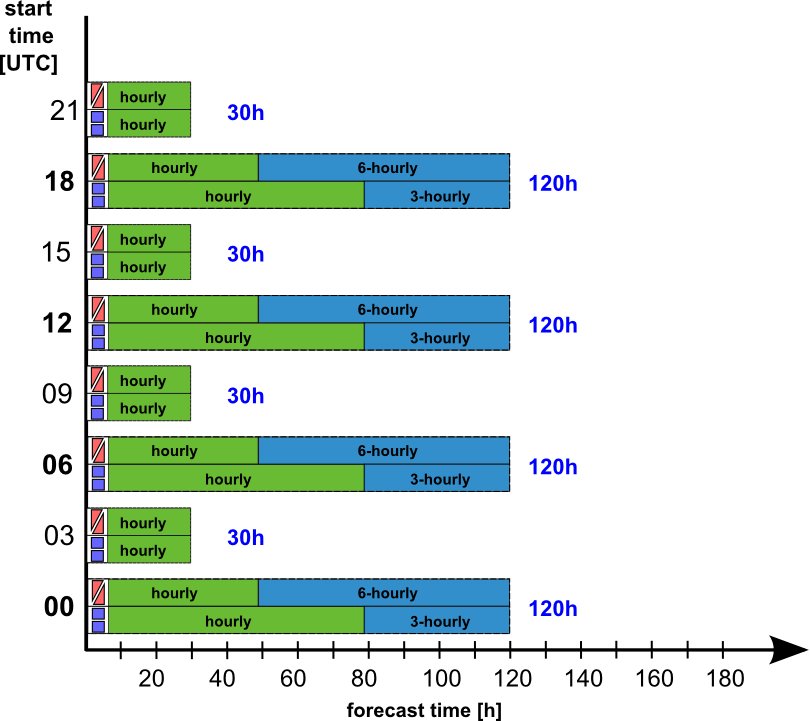
\includegraphics[width=0.92\textwidth]{forecast_length_nest.png}
 \caption{Time span covered by the various EU nest forecasts. A forecast run is launched every three hours.
          Output fields are available hourly up to $VV=78\,\mathrm{h}$ and 3-hourly for larger forecast times. 
          The vertical rules indicate the time until when output is generally available on the native grid 
          (\protect\markRed) and/or on the lat-lon grid (\protect\markBlue). I.e.\ output on the native grid is 
          limited to $VV=48\,\mathrm{h}$.}\label{fig:forecast_length_nest}
\end{figure}

Output is available on two distinct horizontal grids: 
\begin{itemize}
  \item a native triangular grid with an average resolution of $6.5\,\mathrm{km}$, and
  \item a regular latitude-longitude grid with a resolution of $\Delta \lambda = \Delta \Phi=0.0625^{\circ}$.\\
    See Table~\ref{tab:ICON_latlon_summary} for a summary.
\end{itemize}
%
Note that output on the native (triangular) grid is limited to $48\,\mathrm{h}$, whereas output on the regular 
grid is generally available until forecast end. See also Figure \ref{fig:forecast_length_nest}.

Again, in the subsequent tables the availability of specific fields on the native grid ($\,$\markRed$\,$), 
on the lat-lon grid($\,$\markBlue$\,$), or on both grids ($\,$\markRed\markBlue$\,$) is marked in the leftmost 
column. The method used for lat-lon interpolation is indicated in the column \texttt{LL IntpType}.
%
\begin{table}[hbt]
  \centering
  \begin{tabular}{|p{5cm}|p{4.5cm}|p{4.5cm}|}\hline
    \rowcolor{Gray}
                               &    \centering\arraybackslash\textbf{global lat-lon}          &     \centering\arraybackslash\textbf{EU nest lat-lon} \\ \hline\hline
    % ----------------------------------------------------------------------------------------------------------------------------------------
    geogr. coordinates         &    $  0.0^\degree$          -- $359.75^\degree$                     &     $ 23.5^\degree~\text{W}$ -- $62.5^\degree~\text{E}$, \\
                               &    $ 90.0^\degree~\text{S}$ -- $ 90.0^\degree~\text{N}$              &     $ 29.5^\degree~\text{N}$ -- $70.5^\degree~\text{N}$ \\
    mesh size                  &    $0.25^\degree$                                &     $0.0625^\degree$ \\
    \hline
  \end{tabular}
  \caption{Summary of the latitude-longitude grids for ICON global and ICON-EU nest output.}%
  \label{tab:ICON_latlon_summary}
\end{table}


% --------------------------------------------------------------------------------
\subsection{Time-constant (external parameter) fields for the EU nest}
% --------------------------------------------------------------------------------

% LaTeX macros that are later used to disable/enable rows in the
% tables of output fields (global/local domain):
\renewcommand{\onlyglb}[1]{}
\renewcommand{\onlyloc}[1]{#1}
%
\begin{vartable}{\caption{Variables exclusively available for $VV=0$ from the forecast databases (\texttt{CAT\_NAME=\$model\_\$run\_\tblu{fc}\_\$suite}, $s[h]=0$)}\label{table:nest:init_output}}

  % --------- include table of variables
  % 
  \groups[tri][]   & CLAT                          &  Geographical latitude of native grid triangle cell center                              &               0                                   &                     191                     &                    1                       &                 1/--                            &                      inst                   &        $\mathrm{Deg.\, N}$   \\
\groups[tri][]   & CLON                          &  Geographical longitude of native grid triangle cell center                             &               0                                   &                     191                     &                    2                       &                 1/--                            &                      inst                   &        $\mathrm{Deg.\, E}$   \\
\groups[tri][]   & ELAT                          &  Geographical latitude of native grid triangle edge midpoint                            &               0                                   &                     191                     &                    1                       &                 1/--                            &                      inst                   &        $\mathrm{Deg.\, N}$   \\
\groups[tri][]   & ELON                          &  Geographical longitude of native grid triangle edge midpoint                           &               0                                   &                     191                     &                    2                       &                 1/--                            &                      inst                   &        $\mathrm{Deg.\, E}$   \\
\groups[tri][]   & VLAT                          &  Geographical latitude of native grid triangle vertex                                   &               0                                   &                     191                     &                    1                       &                 1/--                            &                      inst                   &        $\mathrm{Deg.\, N}$   \\
\groups[tri][]   & VLON                          &  Geographical longitude of native grid triangle vertex                                  &               0                                   &                     191                     &                    2                       &                 1/--                            &                      inst                   &        $\mathrm{Deg.\, E}$   \\
\groups[tri][ll] & DEPTH\_LK                     &  Lake depth                                                                             &               1                                   &                       2                     &                    0                       &                 1/162                           &                      inst                   &        $\mathrm{m}$ \\
\groups[tri][ll] & FR\_LAND                      &  Land fraction (possible range [$0,1$])                                                 &               2                                   &                       0                     &                    0                       &                 1/--                            &                      inst                   &        $1$ \\
\groups[tri][ll] & FR\_LAKE                      &  Fresh water lake fraction (possible range [$0,1$])                                     &               1                                   &                       2                     &                    2                       &                 1/--                            &                      inst                   &        $1$ \\
\groups[tri][ll] & HHL                           &  Geometric height of model half levels above msl                                        &               0                                   &                       3                     &                    6                       &                 150/101                         &                      inst                   &        $\mathrm{m}$   \\
\groups[tri][ll] & HSURF                         &  Geometric height of the earths surface above msl                                       &               0                                   &                       3                     &                    6                       &                 1/101                           &                      inst                   &        $\mathrm{m}$   \\
\groups[tri][ll] & LAI                           &  Leaf area index                                                                        &               2                                   &                       0                     &                   28                       &                 1/--                            &                      inst                   &        $1$ \\
\groups[tri][]   & NDVIRATIO                     &  ratio of current NDVI (normalized differential vegetation index) to annual max         &               2                                   &                       0                     &                  192                       &                 1/--                            &                      inst                   &        $1$ \\
\groups[tri][ll] & PLCOV                         &  Plant cover                                                                            &               2                                   &                       0                     &                    4                       &                 1/--                            &                      inst                   &        $\mathrm{\%}$ \\
\groups[tri][ll] & ROOTDP                        &  Root depth of vegetation                                                               &               2                                   &                       0                     &                   32                       &                 1/--                            &                      inst                   &        $\mathrm{m}$ \\
\groups[tri][ll] & SOILTYP                       &  Soil type of land fraction  (9 types $[1,\dots, 9]$)                                   &               2                                   &                       3                     &                  196                       &                 1/--                            &                      inst                   &        $1$ \\
  % ------------------------------------

\end{vartable}


% --------------------------------------------------------------------------------
\subsection{Multi-level fields on native hybrid vertical levels for the EU nest}
% --------------------------------------------------------------------------------

% LaTeX macros that are later used to disable/enable rows in the
% tables of output fields (global/local domain):
\renewcommand{\onlyglb}[1]{}
\renewcommand{\onlyloc}[1]{#1}
%
\begin{vartable}{\caption{Hybrid multi-level forecast ($VV>0$) and initialised analysis ($VV=0$) products}}
  
  % --------- include table of variables
  % 
  % TABLE OF VV>0 MULTI-LEVEL FIELDS FROM THE FORECAST DATABASE
%
% This file contains the table data for both the GLOBAL and the EU NEST:
%
% table rows that are only part of the GLOBAL  grid output should be enclosed by         \onlyglb{ ... }
% table rows that are only part of the EU NEST grid output should be enclosed by         \onlyloc{ ... }
%
% ADDITIONAL NOTES:
%
% 1. Variables required to drive INT2LM/COSMO-DE are marked by comment "i2l",
%    see "~for1han/const/iglo/namelst.output.i2l"
%    It is used by script build_varlists.py
%
%    > For the EU nest these are the fields required for the native grid. 
% 
%    ml_varlist           = 'U',         'V',         'W',         'T',         'P',
%                           'QV',        'QC',        'QI',        'QR',        'QS',
%                           'W_I',       'T_G',       'QV_S',
%                           'T_SNOW',    'W_SNOW',    'RHO_SNOW',  'FRESHSNW',
%                           'T_SO',      'W_SO',      'H_ICE',     'T_ICE',
\svnInfo $Id$
\\[-0.5em] % without this dummy line, TikZ does not seem to get the marker position right...
%
%
          \groups[\onlyglb{tri}][         ll ] & CLC                        &  Cloud cover                                                                               &               0/6/22                      &                 150/150                         &                      inst        &             &        $\mathrm{\%}$ \\             
\onlyglb{ \groups[tri          ][            ] & DEN                        &  Density of moist air                                                                      &               0/3/10                      &                 150/150                         &                      inst        &     --      &        $\mathrm{kg\,m^{-3}}$ \\     }
          \groups[tri          ][            ] & DTKE\_CON                  &  Buoyancy-production of TKE due to sub grid scale convection                               &               0/19/219                    &                 150/--                          &                      inst        &     --      &        $\mathrm{m^{2}\,s^{-3}}$ \\   
          \groups[tri          ][            ] & DTKE\_HSH                  &  Production of TKE due to horizontal shear                                                 &               0/19/220                    &                 150/--                          &                      inst        &     --      &        $\mathrm{m^{2}\,s^{-3}}$ \\   
          \groups[tri          ][         ll ] & P                          &  Pressure                                                                                  &               0/3/0                       &                 150/150                         &                      inst        &             &        $\mathrm{Pa}$         \\     % i2l 
          \groups[tri          ][         ll ] & QC                         &  \textcolor{red}{Cloud mixing ratio}\footnotemark[3]                                       &               0/1/22                      &                 150/150                         &                      inst        &             &        $\mathrm{kg\,kg^{-1}}$ \\    % i2l
          \groups[tri          ][         ll ] & QI                         &  \textcolor{red}{Cloud ice mixing ratio}\footnotemark[3]                                   &               0/1/82                      &                 150/150                         &                      inst        &             &        $\mathrm{kg\,kg^{-1}}$ \\    % i2l
          \groups[tri          ][            ] & QR                         &  \textcolor{red}{Rain mixing ratio}\footnotemark[3]                                        &               0/1/24                      &                 150/150                         &                      inst        &     --      &        $\mathrm{kg\,kg^{-1}}$ \\    % i2l
          \groups[tri          ][            ] & QS                         &  \textcolor{red}{Snow mixing ratio}\footnotemark[3]                                        &               0/1/25                      &                 150/150                         &                      inst        &     --      &        $\mathrm{kg\,kg^{-1}}$ \\    % i2l 
          \groups[tri          ][         ll ] & QV                         &  Specific humidity                                                                         &               0/1/0                       &                 150/150                         &                      inst        &             &        $\mathrm{kg\,kg^{-1}}$ \\    % i2l
          \groups[tri          ][         ll ] & T                          &  Temperature                                                                               &               0/0/0                       &                 150/150                         &                      inst        &             &        $\mathrm{K}$          \\     % i2l 
          \groups[tri          ][         ll ] & TKE                        &  Turbulent kinetic energy                                                                  &               0/19/11                     &                 150/--                          &                      inst        &             &        $\mathrm{m^{2}\,s^{-2}}$ \\  
          \groups[tri          ][         ll ] & U                          &  Zonal wind                                                                                &               0/2/2                       &                 150/150                         &                      inst        &             &        $\mathrm{m\,s^{-1}}$   \\    % i2l
          \groups[tri          ][         ll ] & V                          &  Meridional wind                                                                           &               0/2/3                       &                 150/150                         &                      inst        &             &        $\mathrm{m\,s^{-1}}$   \\    % i2l
          \groups[tri          ][         ll ] & W                          &  Vertical wind                                                                             &               0/2/9                       &                 150/--                          &                      inst        &             &        $\mathrm{m\,s^{-1}}$   \\    % i2l


  % ------------------------------------
  
\end{vartable}
\footnotetext[2]{for the time being, erroneously encoded as mixing ratios instead of specific quantities}


% --------------------------------------------------------------------------------
\subsection{Multi-level fields interpolated to pressure levels}
% --------------------------------------------------------------------------------

\renewcommand{\new}[1]{\textcolor{red}{#1}}
%
% List of pressure levels taken from COSMO-EU DB documentation, Section 5.1 (2015-03-27)
%
\renewcommand{\pressurelevelsRegular}{$1000$, \new{$975$}, $950$, \new{$925$}, \new{$900$}, 
                                    \new{$875$}, $850$, \new{$825$}, \new{$800$}, 
                                    \new{$775$}, \new{$750$}, \new{$725$}, $700$, $600$, 
                                    $500$, $400$, $300$, $250$, $200$, \new{$150$}, \new{$100$}, 
                                    \new{$70$}, \new{$50$}~$\mathrm{hPa}$}

For regular grid output the following pressure levels are available: 
\begin{center}
\begin{minipage}{0.5\linewidth}
\pressurelevelsRegular. 
\end{minipage}
\end{center}

Newly available pressure levels (as compared to COSMO-EU) are highlighted in red. 
The output fields are listed in Table~\ref{table:nest:output_pressurelevels_regular}.

On the native (triangular) grid no output is generated for pressure levels.

\renewcommand{\new}[1]{#1}

\begin{vartable}{\caption{Regular grid output on the ICON EU Nest:
      Multi-level forecast ($VV>0$) and initialised analysis ($VV=0$) products 
      interpolated to pressure levels \pressurelevelsRegular.}\label{table:nest:output_pressurelevels_regular}}
  
  \groups[][ll] & FI                         &  Geopotential                                                                              &               0/3/4                       &                 100/--                          &                      inst     &              &        $\mathrm{m^{2}\,s^{-2}}$   \\ % pl
  \groups[][ll] & OMEGA                      &  Vertical velocity in pressure coordinates ($\omega=\mathrm{d}p/\mathrm{d}t$)              &               0/2/8                       &                 100/--                          &                      inst     &              &        $\mathrm{Pa\,s^{-1}}$  \\     % pl
  \groups[][ll] & RELHUM                     &  Relative humidity (with respect to water)                                                 &               0/1/1                       &                 100/--                          &                      inst     &              &        $\mathrm{\%}$          \\     % pl
  \groups[][ll] & T                          &  Temperature                                                                               &               0/0/0                       &                 100/--                          &                      inst     &              &        $\mathrm{K}$          \\      % pl
  \groups[][ll] & U                          &  Zonal wind                                                                                &               0/2/2                       &                 100/--                          &                      inst     &              &        $\mathrm{m\,s^{-1}}$   \\     % pl
  \groups[][ll] & V                          &  Meridional wind                                                                           &               0/2/3                       &                 100/--                          &                      inst     &              &        $\mathrm{m\,s^{-1}}$   \\     % pl
  
\end{vartable}



%% --------------------------------------------------------------------------------
%\subsection{Multi-level fields interpolated to height levels}
%% --------------------------------------------------------------------------------
%
%
%%
%% List of pressure levels taken from COSMO-EU DB documentation, Section 5.1 (2015-03-27)
%%
%\renewcommand{\heightlevelsRegular}{$10000$, $5000$, $3000$, $2000$, $1500$, $1000$, $500$, $100$~$\mathrm{m}$}
%
%\begin{vartable}{\caption{Regular grid output on the ICON EU Nest:
%      Multi-level forecast ($VV>0$) and initialised analysis ($VV=0$) products interpolated to height levels \heightlevelsRegular
%      ~(above mean sea level).}\label{table:nest:output_heightlevels_regular}}
%  
%  \groups[][ll] & U                          &  Zonal wind                                                                                &               0                                   &                     2                       &                    2                       &                 102/--                          &                      inst                   &        $\mathrm{m\,s^{-1}}$   \\ % pl
%  \groups[][ll] & V                          &  Meridional wind                                                                           &               0                                   &                     2                       &                    3                       &                 102/--                          &                      inst                   &        $\mathrm{m\,s^{-1}}$   \\ % pl
%  \groups[][ll] & W                          &  Vertical wind                                                                             &               0                                   &                     2                       &                    9                       &                 102/--                          &                      inst                   &        $\mathrm{m\,s^{-1}}$   \\ % pl
%  \groups[][ll] & T                          &  Temperature                                                                               &               0                                   &                     0                       &                    0                       &                 102/--                          &                      inst                   &        $\mathrm{K}$          \\  % pl
%  \groups[][ll] & P                          &  Pressure                                                                                  &               0                                   &                     3                       &                    0                       &                 102/--                          &                      inst                   &        $\mathrm{Pa}$         \\  % pl
%
%\end{vartable}
%


% --------------------------------------------------------------------------------
\subsection{Single-level fields}
% --------------------------------------------------------------------------------

% LaTeX macros that are later used to disable/enable rows in the
% tables of output fields (global/local domain):
\renewcommand{\onlyglb}[1]{}
\renewcommand{\onlyloc}[1]{#1}
%
\begin{vartable}{\caption[]{Single-level forecast ($VV>0$) and initialised analysis ($VV=0$) products on the ICON EU Nest}}

  % --------- include table of variables
  % TABLE OF VV>0 MULTI-LEVEL FIELDS FROM THE FORECAST DATABASE
%
% This file contains the table data for both the GLOBAL and the EU NEST:
%
% table rows that are only part of the GLOBAL  grid output should be enclosed by         \onlyglb{ ... }
% table rows that are only part of the EU NEST grid output should be enclosed by         \onlyloc{ ... }
%
% ADDITIONAL NOTES:
%
% 1. Variables required to drive INT2LM/COSMO-DE are marked by comment "i2l",
%    see "~for1han/const/iglo/namelst.output.i2l"
%    It is used by script build_varlists.py
%
%    > For the EU nest these are the fields required for the native grid. 
% 
%    ml_varlist           = 'U',         'V',         'W',         'T',         'P',
%                           'QV',        'QC',        'QI',        'QR',        'QS',
%                           'W_I',       'T_G',       'QV_S',
%                           'T_SNOW',    'W_SNOW',    'RHO_SNOW',  'FRESHSNW',
%                           'T_SO',      'W_SO',      'H_ICE',     'T_ICE',
%
%
\svnInfo $Id$
\\[-0.5em] % without this dummy line, TikZ does not seem to get the marker position right...
%
%
           \groups[\onlyglb{tri}][         ll ] & ALB\_RAD                       &  Shortwave broadband albedo for diffuse radiation                                      &               0                                   &                    19                       &                     1                      &                 1/--                            &                      inst                   &        $\mathrm{\%}$    \\            
           \groups[\onlyglb{tri}][         ll ] & ALHFL\_S                       &  Latent heat net flux at surface (average since model start)                           &               0                                   &                     0                       &                    10                      &                 1/--                            &                      avg                    &        $\mathrm{W\,m^{-2}}$  \\
           \groups[             ][         ll ] & APAB\_S                        &  Photosynthetically active radiation flux at surface (average since model start)       &               0                                   &                     4                       &                    10                      &                 1/--                            &                      avg                    &        $\mathrm{W\,m^{-2}}$    \\    
           \groups[\onlyglb{tri}][         ll ] & ASHFL\_S                       &  Sensible heat net flux at surface (average since model start)                         &               0                                   &                     0                       &                    11                      &                 1/--                            &                      avg                    &        $\mathrm{W\,m^{-2}}$  \\
           \groups[\onlyglb{tri}][         ll ] & ASOB\_S                        &  Net short-wave radiation flux at surface (average since model start)                  &               0                                   &                     4                       &                     9                      &                 1/--                            &                      avg                    &        $\mathrm{W\,m^{-2}}$    \\    
           \groups[\onlyglb{tri}][         ll ] & ASOB\_T                        &  Net short-wave radiation flux at TOA (average since model start)                      &               0                                   &                     4                       &                     9                      &                 8/--                            &                      avg                    &        $\mathrm{W\,m^{-2}}$    \\    
           \groups[\onlyglb{tri}][         ll ] & ASWDIFD\_S                     &  Surface down solar diffuse radiation (average since model start)                      &               0                                   &                     4                       &                   199                      &                 1/--                            &                      avg                    &        $\mathrm{W\,m^{-2}}$  \\      
           \groups[\onlyglb{tri}][         ll ] & ASWDIFU\_S                     &  Surface up solar diffuse radiation (average since model start)                        &               0                                   &                     4                       &                     8                      &                 1/--                            &                      avg                    &        $\mathrm{W\,m^{-2}}$  \\      
           \groups[\onlyglb{tri}][         ll ] & ASWDIR\_S                      &  Surface down solar direct radiation (average since model start)                       &               0                                   &                     4                       &                   198                      &                 1/--                            &                      avg                    &        $\mathrm{W\,m^{-2}}$  \\      
           \groups[\onlyglb{tri}][         ll ] & ATHB\_S                        &  Net long-wave radiation flux at surface (average since model start)                   &               0                                   &                     5                       &                     5                      &                 1/--                            &                      avg                    &        $\mathrm{W\,m^{-2}}$    \\    
           \groups[\onlyglb{tri}][         ll ] & ATHB\_T                        &  Net long-wave radiation flux at TOA (average since model start)                       &               0                                   &                     5                       &                     5                      &                 8/--                            &                      avg                    &        $\mathrm{W\,m^{-2}}$    \\    
           \groups[\onlyglb{tri}][         ll ] & AUMFL\_S                       &  U-momentum flux at surface $\overline{u^{\prime}w^{\prime}}^{1/2}$ (average since model start)&       0                                   &                     2                       &                    17                      &                 1/--                            &                      avg                    &        $\mathrm{m}$  \\ 
           \groups[\onlyglb{tri}][         ll ] & AVMFL\_S                       &  V-momentum flux at surface $\overline{v^{\prime}w^{\prime}}^{1/2}$ (average since model start)&       0                                   &                     2                       &                    18                      &                 1/--                            &                      avg                    &        $\mathrm{m}$  \\ 
           \groups[\onlyglb{tri}][\onlyloc{ll}] & CAPE\_CON                      &  Convective available potential energy                                                 &               0                                   &                     7                       &                     6                      &                 1/--                            &                      inst                   &        $\mathrm{J\,kg^{-1}}$  \\  
           \groups[\onlyglb{tri}][         ll ] & CLCH                           &  High level clouds                                                                     &               0                                   &                     6                       &                    22                      &                 100/100                         &                      inst                   &        $\mathrm{\%}$          \\    
           \groups[\onlyglb{tri}][         ll ] & CLCM                           &  Mid level clouds                                                                      &               0                                   &                     6                       &                    22                      &                 100/100                         &                      inst                   &        $\mathrm{\%}$          \\    
           \groups[\onlyglb{tri}][         ll ] & CLCL                           &  Low level clouds                                                                      &               0                                   &                     6                       &                    22                      &                 100/1                           &                      inst                   &        $\mathrm{\%}$          \\    
           \groups[\onlyglb{tri}][         ll ] & CLCT                           &  Total cloud cover                                                                     &               0                                   &                     6                       &                     1                      &                 1/--                            &                      inst                   &        $\mathrm{\%}$          \\    
           \groups[             ][         ll ] & CLCT\_MOD                      &  Modified total cloud cover for media                                                  &               0                                   &                     6                       &                   199                      &                 1/--                            &                      inst                   &        $1$                    \\     
           \groups[             ][         ll ] & CLDEPTH                        &  Modified cloud depth for media                                                        &               0                                   &                     6                       &                   198                      &                 1/--                            &                      inst                   &        $1$                    \\     
           \groups[         tri ][            ] & FRESHSNW                       &  Fresh snow factor (weighting function for albedo indicating freshness of snow)        &               0                                   &                     1                       &                   203                      &                 1/--                            &                      inst                   &        $1$  \\                       % i2l
           \groups[         tri ][            ] & FR\_ICE                        &  Sea/lake ice cover  (possible range: $[0,1]$)                                         &              10                                   &                     2                       &                     0                      &                 1/--                            &                      inst                   &        $1$  \\
           \groups[\onlyglb{tri}][         ll ] & HBAS\_CON                      &  Height of convective cloud base above msl                                             &               0                                   &                     6                       &                    26                      &                 2/101                           &                      inst                   &        $\mathrm{m}$  \\              
           \groups[         tri ][         ll ] & H\_ICE                         &  Sea/Lake ice thickness (Max: $3\,\mathrm{m}$)                                         &              10                                   &                     2                       &                     1                      &                 1/--                            &                      inst                   &        $\mathrm{m}$  \\             % i2l
           \groups[\onlyglb{tri}][         ll ] & H\_SNOW                        &  Snow depth                                                                            &               0                                   &                     1                       &                    11                      &                 1/--                            &                      inst                   &        $\mathrm{m}$  \\              
           \groups[\onlyglb{tri}][         ll ] & HTOP\_CON                      &  Height of convective cloud top above msl                                              &               0                                   &                     6                       &                    27                      &                 3/101                           &                      inst                   &        $\mathrm{m}$  \\              
           \groups[\onlyglb{tri}][         ll ] & HTOP\_DC                       &  Height of top of dry convection above msl                                             &               0                                   &                     6                       &                   196                      &                 3/101                           &                      inst                   &        $\mathrm{m}$  \\              
           \groups[\onlyglb{tri}][         ll ] & HZEROCL                        &  Height of 0 degree Celsius isotherm above msl                                         &               0                                   &                     3                       &                     6                      &                 4/101                           &                      inst                   &        $\mathrm{m}$  \\              
           \groups[             ][         ll ] & PMSL                           &  Surface pressure reduced to msl                                                       &               0                                   &                     3                       &                     1                      &                 101/--                          &                      inst                   &        $\mathrm{Pa}$   \\
           \groups[\onlyglb{tri}][         ll ] & PS                             &  Surface pressure (not reduced)                                                        &               0                                   &                     3                       &                    0                       &                 1/--                            &                      inst                   &        $\mathrm{Pa}$   \\            
           \groups[             ][         ll ] & QV\_2M                         &  Specific humidity at 2m above ground                                                  &               0                                   &                     1                       &                     0                      &               103/--                            &                      inst                   &        $\mathrm{kg\,kg^{-1}}$ \\
           \groups[         tri ][         ll ] & QV\_S                          &  Surface specific humidity                                                             &               0                                   &                     1                       &                    0                       &                 1/--                            &                      inst                   &        $\mathrm{kg\,kg^{-1}}$    \\ % i2l 
           \groups[\onlyglb{tri}][         ll ] & RAIN\_CON\onlyglb{\footnotemark[4]} &  Convective rain (accumulated since model start)                                  &               0                                   &                     1                       &                    76                      &                 1/--                            &                      accu                   &        $\mathrm{kg\,m^{-2}}$    \\   
           \groups[\onlyglb{tri}][         ll ] & RAIN\_GSP\onlyglb{\footnotemark[4]} &  Large scale rain (accumulated since model start)                                 &               0                                   &                     1                       &                    77                      &                 1/--                            &                      accu                   &        $\mathrm{kg\,m^{-2}}$    \\   
           \groups[             ][         ll ] & RELHUM\_2M                     &  Relative humidity at 2m above ground                                                  &               0                                   &                     1                       &                     1                      &               103/--                            &                      inst                   &        $\mathrm{\%}$     \\          
           \groups[         tri ][         ll ] & RHO\_SNOW                      &  Snow density                                                                          &               0                                   &                     1                       &                    61                      &                 1/--                            &                      inst                   &        $\mathrm{kg\,m^{-3}}$  \\     % i2l
 \onlyglb{ \groups[         tri ][            ] & RSTOM                          &  Stomatal resistance                                                                   &               2                                   &                     0                       &                   195                      &                 1/--                            &                      inst                   &        $\mathrm{s\,m^{-1}}$  \\     }
           \groups[\onlyglb{tri}][         ll ] & RUNOFF\_G                      &  Soil water runoff (accumulated since model start)                                     &               2                                   &                     0                       &                     5                      &                 106/--                          &                      accu                   &        $\mathrm{kg\,m^{-2}}$  \\                                    
           \groups[\onlyglb{tri}][         ll ] & RUNOFF\_S                      &  Surface water runoff (accumulated since model start)                                  &               2                                   &                     0                       &                     5                      &                 106/--                          &                      accu                   &        $\mathrm{kg\,m^{-2}}$  \\     
           \groups[\onlyglb{tri}][         ll ] & SNOW\_CON\onlyglb{\footnotemark[4]} &  Convective snowfall water equivalent (accumulated since model start)             &               0                                   &                     1                       &                    55                      &                 1/--                            &                      accu                   &        $\mathrm{kg\,m^{-2}}$    \\   
           \groups[\onlyglb{tri}][         ll ] & SNOW\_GSP\onlyglb{\footnotemark[4]} &  Large snowfall water equivalent (accumulated since model start)                  &               0                                   &                     1                       &                    56                      &                 1/--                            &                      accu                   &        $\mathrm{kg\,m^{-2}}$    \\   
 \onlyloc{ \groups[             ][         ll ] & SNOWLMT\footnotemark[5]        &  Height of snowfall limit above MSL                                                    &               0                                   &                     1                       &                   204                      &                 4/101                           &                      inst                   &        $\mathrm{m}$    \\   }
 \onlyglb{ \groups[             ][         ll ] & SOBS\_RAD                      &  Net short-wave radiation flux at surface (instantaneous)                              &               0                                   &                     4                       &                     9                      &                 1/--                            &                      inst                   &        $\mathrm{W\,m^{-2}}$    \\    }
           \groups[\onlyglb{tri}][         ll ] & T\_2M                          &  Temperature at 2m above ground                                                        &               0                                   &                     0                       &                     0                      &               103/--                            &                      inst                   &        $\mathrm{K}$          \\      
           \groups[\onlyglb{tri}][         ll ] & TCH                            &  Turbulent transfer coefficient for heat and moisture (surface)                        &               0                                   &                     0                       &                    19                      &                 1/--                            &                      inst                   &        $1$    \\ 
           \groups[\onlyglb{tri}][         ll ] & TCM                            &  Turbulent transfer coefficient for momentum (surface)                                 &               0                                   &                     2                       &                    29                      &                 1/--                            &                      inst                   &        $1$    \\ 
           \groups[\onlyglb{tri}][         ll ] & TD\_2M                         &  Dew point temperature at 2m above ground                                              &               0                                   &                     0                       &                     6                      &               103/--                            &                      inst                   &        $\mathrm{K}$          \\      
           \groups[         tri ][         ll ] & T\_G                           &  Ground temperature (temperature at sfc-atm interface)                                 &               0                                   &                     0                       &                    0                       &                 1/--                            &                      inst                   &        $\mathrm{K}$    \\           % i2l
 \onlyglb{ \groups[             ][         ll ] & THBS\_RAD                      &  Net long-wave radiation flux at surface (instantaneous)                               &               0                                   &                     5                       &                     5                      &                 1/--                            &                      inst                   &        $\mathrm{W\,m^{-2}}$    \\    }
           \groups[         tri ][         ll ] & T\_ICE                         &  Sea/Lake ice temperature (at ice-atm interface)                                       &              10                                   &                     2                       &                     8                      &                 1/--                            &                      inst                   &        $\mathrm{K}$  \\             % i2l 
           \groups[\onlyglb{tri}][         ll ] & TMAX\_2M                       &  Maximum temperature at 2m above ground                                                &               0                                   &                     0                       &                     0                      &               103/--                            &                      max                    &        $\mathrm{K}$          \\     
           \groups[\onlyglb{tri}][         ll ] & TMIN\_2M                       &  Minimum temperature at 2m above ground                                                &               0                                   &                     0                       &                     0                      &               103/--                            &                      min                    &        $\mathrm{K}$          \\     
           \groups[\onlyglb{tri}][         ll ] & TOT\_PREC\onlyglb{\footnotemark[4]} &  Total precipitation (accumulated since model start)                              &               0                                   &                     1                       &                    52                      &                 1/--                            &                      accu                   &        $\mathrm{kg\,m^{-2}}$  \\     
           \groups[\onlyglb{tri}][         ll ] & TQC                            &  Column integrated cloud water (grid scale)                                            &               0                                   &                     1                       &                    69                      &                 1/--                            &                      inst                   &        $\mathrm{kg\,m^{-2}}$  \\    
 \onlyglb{ \groups[         tri ][         ll ] & TQC\_DIA                       &  Total column integrated cloud water (including sub-grid-scale contribution)           &               0                                   &                     1                       &                   215                      &                 1/--                            &                      inst                   &        $\mathrm{kg\,m^{-2}}$  \\    }
           \groups[\onlyglb{tri}][         ll ] & TQI                            &  Column integrated cloud ice (grid scale)                                              &               0                                   &                     1                       &                    70                      &                 1/--                            &                      inst                   &        $\mathrm{kg\,m^{-2}}$  \\    
 \onlyglb{ \groups[         tri ][         ll ] & TQI\_DIA                       &  Total column integrated cloud ice (including sub-grid-scale contribution)             &               0                                   &                     1                       &                   216                      &                 1/--                            &                      inst                   &        $\mathrm{kg\,m^{-2}}$  \\    }
           \groups[\onlyglb{tri}][         ll ] & TQR                            &  Column integrated rain (grid scale)                                                   &               0                                   &                     1                       &                    45                      &                 1/--                            &                      inst                   &        $\mathrm{kg\,m^{-2}}$  \\
           \groups[\onlyglb{tri}][         ll ] & TQS                            &  Column integrated snow (grid scale)                                                   &               0                                   &                     1                       &                    46                      &                 1/--                            &                      inst                   &        $\mathrm{kg\,m^{-2}}$  \\ 
           \groups[\onlyglb{tri}][         ll ] & TQV                            &  Column integrated water vapour (grid scale)                                           &               0                                   &                     1                       &                    64                      &                 1/--                            &                      inst                   &        $\mathrm{kg\,m^{-2}}$  \\    
           \groups[\onlyglb{tri}][\onlyloc{ll}] & T\_S                           &  Temperature of the soil surface (equivalent to T\_SO(0))                              &               2                                   &                     3                       &                    18                      &                 1/--                            &                      inst                   &        $\mathrm{K}$    \\             
           \groups[         tri ][         ll ] & T\_SNOW                        &  Temperature of the snow surface                                                       &               0                                   &                     0                       &                    18                      &                 1/--                            &                      inst                   &        $\mathrm{K}$    \\            % i2l
           \groups[\onlyglb{tri}][         ll ] & U\_10M                         &  Zonal wind at 10m above ground                                                        &               0                                   &                     2                       &                     2                      &               103/--                            &                      inst                   &        $\mathrm{m\,s^{-1}}$  \\      
           \groups[\onlyglb{tri}][         ll ] & V\_10M                         &  Meridional wind at 10m above ground                                                   &               0                                   &                     2                       &                     3                      &               103/--                            &                      inst                   &        $\mathrm{m\,s^{-1}}$  \\      
           \groups[\onlyglb{tri}][         ll ] & VMAX\_10M                      &  Maximum wind at $10\,\mathrm{m}$ above ground                                         &               0                                   &                     2                       &                    22                      &               103/--                            &                      max                    &        $\mathrm{m\,s^{-1}}$   \\     
           \groups[         tri ][            ] & W\_I                           &  Plant canopy surface water                                                            &               2                                   &                     0                       &                    13                      &                 1/--                            &                      inst                   &        $\mathrm{kg\,m^{-2}}$    \\ % i2l
           \groups[         tri ][         ll ] & W\_SNOW                        &  Snow depth water equivalent                                                           &               0                                   &                     1                       &                    60                      &                 1/--                            &                      inst                   &        $\mathrm{kg\,m^{-2}}$    \\    % i2l
           \groups[\onlyglb{tri}][         ll ] & WW                             &  Weather interpretation  (WMO)                                                         &               0                                   &                    19                       &                    25                      &                 1/--                            &                      inst                   &        $1$ \\                        
           \groups[\onlyglb{tri}][         ll ] & Z0                             &  Surface roughness (above land and water)                                              &               2                                   &                     0                       &                     1                      &                 1/--                            &                      inst                   &        $\mathrm{m}$          \\      

  % ------------------------------------

\end{vartable}

\footnotetext[5]{T\_S is identical to T\_SO at level 0. It will no longer be available in the future. Use T\_SO(0) instead of T\_S.} 


% --------------------------------------------------------------------------------
\subsection{Soil-specific multi-level fields}
% --------------------------------------------------------------------------------


%    Variables required to drive INT2LM/COSMO-DE,
%    see "~for1han/const/iglo/namelst.output.i2l"
%
%    > For the EU nest these are the fields required for the native grid. 
% 
%      'T_SO',      'W_SO'

\begin{vartable}{\caption[]{Multi-level forecast ($VV>0$) and initialised analysis ($VV=0$) products of the soil model}}

  \groups[tri][ll] & T\_SO                          &  Soil temperature                                                                      &               2/3/18                       &               106/--                           &                      inst       &               &        $\mathrm{K}$   \\           % i2l
  \groups[tri][ll] & W\_SO                          &  Soil moisture integrated over individual soil layers  (ice + liquid)                  &               2/3/20                       &               106/106                          &                      inst       &               &        $\mathrm{kg\,m^{-2}}$   \\  % i2l
  \groups[tri][ll] & W\_SO\_ICE                     &  Soil ice content integrated over individual soil layers                               &               2/3/22                       &               106/106                          &                      inst       &     NNB       &        $\mathrm{kg\,m^{-2}}$   \\
  
\end{vartable}

Soil temperature is defined at the soil depths given in Table \ref{table:nest:soillayer} (column 2). Levels $1$ to $8$ define the full levels of the soil model. A zero gradient 
condition is assumed between levels $0$ and $1$, meaning that temperatures at the surface-atmosphere interface are set equal to the temperature at the first full level depth.
($0.5\,\mathrm{cm}$). Temperatures are prognosed for layers $1$ to $7$. At the lowermost layer (mid-level height $1458\,\mathrm{cm}$) the temperature is fixed 
to the climatological average $2\,\mathrm{m}$-temperature.

Soil moisture \texttt{W\_SO} is prognosed for layers $1$ to $6$. In the two lowermost layers \texttt{W\_SO} is filled with \texttt{W\_SO(6)} (zero gradient condition).
\begin{table}[H]
\center
\caption{Soil model: vertical distribution of levels and layers}\label{table:nest:soillayer}
 \begin{tabular}{>{\centering\arraybackslash}p{2.0cm}>{\centering\arraybackslash}p{2.5cm}|>{\centering\arraybackslash}p{2.5cm}>{\centering\arraybackslash}p{5.0cm}}
 \toprule
  \bf{level no.}       &  \bf{depth [cm]}        &   \bf{layer no.}        & \bf{upper/lower bounds [cm]} \\
 \midrule
         0             &     $0.0$               &                         &                                     \\
         1             &     $0.5$               &         1               &     $0.0$\, \textemdash\, $1.0$     \\
         2             &     $2.0$               &         2               &     $1.0$\, \textemdash\, $3.0$     \\
         3             &     $6.0$               &         3               &     $3.0$\, \textemdash\, $9.0$     \\
         4             &     $18.0$              &         4               &     $9.0$\, \textemdash\, $27.0$    \\
         5             &     $54.0$              &         5               &    $27.0$\, \textemdash\, $81.0$    \\
         6             &     $162.0$             &         6               &    $81.0$\, \textemdash\, $243.0$   \\
         7             &     $486.0$             &         7               &   $243.0$\, \textemdash\, $729.0$   \\
         8             &     $1458.0$            &         8               &   $729.0$\, \textemdash\, $2187.0$  \\
 \bottomrule
 \end{tabular}
\end{table}




% --------------------------------------------------------------------------------
\subsection{Lake-specific single-level fields}
% --------------------------------------------------------------------------------


%\begin{vartable}{\caption[]{Initialised analysis ($VV=0$) products of the lake model model on the ICON EU nest.}}

%  \groups[tri][  ] & C\_T\_LK                       &  Shape factor with respect to the temperature profile in the thermocline               &               1                                   &                     2                       &                    10                       &               162/166                          &                      inst                   &        $1$    \\
%  \groups[tri][  ] & H\_ML\_LK                      &  Mixed-layer depth                                                                     &               1                                   &                     2                       &                     0                       &                 1/166                          &                      inst                   &        $\mathrm{m}$ \\
%  \groups[tri][  ] & T\_BOT\_LK                     &  Temperature at the water-bottom sediment interface                                    &               1                                   &                     2                       &                     1                       &               162/--                           &                      inst                   &        $\mathrm{K}$ \\
%  \groups[tri][  ] & T\_MNW\_LK                     &  Mean temperature of the water column                                                  &               1                                   &                     2                       &                     1                       &                 1/162                          &                      inst                   &        $\mathrm{K}$ \\
%  \groups[tri][  ] & T\_WML\_LK                     &  Mixed-layer temperature                                                               &               1                                   &                     2                       &                     1                       &                 1/166                          &                      inst                   &        $\mathrm{K}$ \\

%\end{vartable}


\begin{vartable}{\caption[]{Single-level forecast ($VV>0$) and initialised analysis ($VV=0$) products of the lake model model on the ICON EU nest.}}

  \groups[tri][] & C\_T\_LK                       &  Shape factor with respect to the temperature profile in the thermocline               &               1/2/10                      &               162/166                          &                      inst     &     --         &        $1$    \\
  \groups[tri][] & H\_ML\_LK                      &  Mixed-layer depth                                                                     &               1/2/0                       &                 1/166                          &                      inst     &     --         &        $\mathrm{m}$ \\
  \groups[tri][] & T\_BOT\_LK                     &  Temperature at the water-bottom sediment interface                                    &               1/2/1                       &               162/--                           &                      inst     &     --         &        $\mathrm{K}$ \\
  \groups[tri][] & T\_MNW\_LK                     &  Mean temperature of the water column                                                  &               1/2/1                       &                 1/162                          &                      inst     &     --         &        $\mathrm{K}$ \\
  \groups[tri][] & T\_WML\_LK                     &  Mixed-layer temperature                                                               &               1/2/1                       &                 1/166                          &                      inst     &     --         &        $\mathrm{K}$ \\
  
\end{vartable}

%\svnInfo $Id$

\newpage
%
% --------------------------------------------------------------------------------
\section{COSMO-EU fields which are not yet available in ICON}
% --------------------------------------------------------------------------------

\begin{vartable}{\caption{Variables exclusively available for $VV=0$ from the forecast databases (\texttt{CAT\_NAME=\$model\_\$run\_\tblu{fc}\_\$suite}, $s[h]=0$)}\label{table_constdb}}

  \groups[][ll]   & \st{FIS}\footnotemark[2]    &  surface geopotential                                       &               0                                   &                       3                     &                    4                       &                 1/--                          &                      inst                   &        $\mathrm{m^{2}\, s^{-2}}$   \\
  \groups[][ll]   & \st{RLAT}                   &  geographical latitude                                      &               0                                   &                     191                     &                    1                       &                 1/--                          &                      inst                   &        Deg.\ N   \\
  \groups[][ll]   & \st{RLON}                   &  geographical longitude                                     &               0                                   &                     191                     &                    2                       &                 1/--                          &                      inst                   &        Deg.\ E   \\
  \groups[][ll]   & \st{FC}                     &  Coriolis parameter                                         &               0                                   &                      19                     &                  193                       &                 1/--                          &                      inst                   &        $\mathrm{s^{-1}}$ \\
  \groups[][ll]   & \st{HMO3}                   &  height of maximum Ozone concentration                      &               0                                   &                      14                     &                  192                       &                 1/--                          &                      inst                   &        $\mathrm{Pa}$ \\
  \groups[][ll]   & \st{VIO3}                   &  vertically integrated Ozone                                &               0                                   &                      14                     &                  193                       &                 1/--                          &                      inst                   &        $\mathrm{Pa}$ \\
  \groups[][ll]   & ALB\_DIF                    &  diffusive albedo                                     &               0                                   &                      19                     &                   18                       &                 1/--                          &                      inst                   &        $1$       \\
  
\end{vartable}

Lat-Lon output missing for \texttt{FOR\_E}, \texttt{FOR\_D}.



\begin{vartable}{\caption{Hybrid multi-level forecast ($VV>0$) and initialised analysis ($VV=0$) products}}
  
  \groups[][ll] & \st{PP}\footnotemark[2]     &  Pressure anomaly                                                                            &               3                                   &                   192                       &                  150                       &                 150/--                         &                      inst                   &        $\mathrm{hPa}$   \\ 
  \groups[][ll] & \st{Q\_SEDIM}\footnotemark[3] &  specific mass of sedimenting particles                                                      &               0                                   &                     1                       &                  196                       &                 150/150                        &                      inst                   &        $\mathrm{kg\, kg^{-1}}$   \\ 
  \groups[][ll] & \st{TKVM}\footnotemark[1]   &  Turbulent diffusion coefficient for momentung                                               &               0                                   &                     2                       &                   31                       &                 150/--                         &                      inst                   &        $\mathrm{m^{2}\, s^{-1}}$\\
  \groups[][ll] & \st{TKVH}\footnotemark[1]   &  Turbulent diffusion coefficient for heat and moisture                                       &               0                                   &                     0                       &                   20                       &                 150/--                         &                      inst                   &        $\mathrm{m^{2}\, s^{-1}}$\\
  
\end{vartable}

Lat-Lon output missing for \texttt{QR}, \texttt{QS}.


\begin{vartable}{\caption[]{Single-level forecast ($VV>0$) and initialised analysis ($VV=0$) products}}

\groups[][ll] & \st{T\_M}\footnotemark[2]      &  Temperature at the upper boundary of the midlevel soil layer            &               2                                   &                     3                       &                   18                       &                106/--                            &                      inst                   &        $\mathrm{K}$   \\ 
\groups[][ll] & \st{W\_G1}\footnotemark[2]     &  Water content of uppermost soil layer                                   &               2                                   &                     3                       &                   20                       &                106/106                           &                      inst                   &        $\mathrm{kg\, m^{-2}}$ \\ 
\groups[][ll] & \st{W\_G2}\footnotemark[2]     &  Water content of midlevel soil layer                                    &               2                                   &                     3                       &                   20                       &                106/106                           &                      inst                   &        $\mathrm{kg\, m^{-2}}$ \\
\groups[][ll] & AEVAP\_S                       &  Surface moisture flux (accumulated sice model start)                    &               0                                   &                     1                       &                   79                       &                  1/--                            &                      accu                   &        $\mathrm{kg\, m^{-2}}$ \\
\groups[][ll] & TDIV\_HUM                      &  Vertically integrated divergence of specific humidity (accumulated sice model start) &  0                                   &                     1                       &                  192                       &                  1/--                            &                      accu                   &        $\mathrm{kg\, m^{-2}}$ \\
\groups[][ll] & TWATER                         &  Vertically integrated water                                             &               0                                   &                     1                       &                   78                       &                  1/--                            &                      inst                   &        $\mathrm{kg\, m^{-2}}$ \\
\groups[][ll] & BAS\_CON                       &  Level index of convective cloud base                                    &               0                                   &                     6                       &                  194                       &                  1/--                            &                      inst                   &        $1$ \\
\groups[][ll] & TOP\_CON                       &  Level index of convective cloud top                                     &               0                                   &                     6                       &                  195                       &                  1/--                            &                      inst                   &        $1$ \\
\groups[][ll] & SNOWLMT                        &  Snow line height above msl                                              &               0                                   &                     1                       &                  204                       &                  4/--                            &                      inst                   &        $\mathrm{m}$ \\
\groups[][ll] & CAPE\_ML                       &  Mixed layer CAPE                                                        &               0                                   &                     7                       &                    6                       &                192/--                            &                      inst                   &        $\mathrm{J\, kg^{-1}}$ \\
\groups[][ll] & CIN\_ML                        &  Mixed layer CIN                                                         &               0                                   &                     7                       &                    7                       &                192/--                            &                      inst                   &        $\mathrm{J\, kg^{-1}}$ \\
\groups[][ll] & ZHD                            &  Delay of the GPS signal through dry atmos.                   &               0                                   &                    15                       &                  194                       &                  1/--                            &                      inst                   &        $\mathrm{m}$ \\
\groups[][ll] & ZWD                            &  Delay of the GPS signal through wet atmos.                    &               0                                   &                    15                       &                  193                       &                  1/--                            &                      inst                   &        $\mathrm{m}$ \\
\groups[][ll] & ZTD                            &  Delay of the GPS signal through the (total) atm.                                &               0                                   &                    15                       &                  192                       &                  1/--                            &                      inst                   &        $\mathrm{m}$ \\

\end{vartable}

Lat-Lon output missing for \texttt{T\_S}, \texttt{W\_I}, \texttt{FRESHSNW}, \texttt{CAPE\_CON}, \texttt{DTKE\_CON}. By the way: isn't \texttt{DTKE\_CON} a 3D-field? 
For COSMO-EU it is listed in the table for single level fields.


\begin{vartable}{\caption{Regular grid output:
      Multi-level forecast ($VV>0$) and initialised analysis ($VV>0$) products interpolated to height levels \heightlevelsRegular
      ~(above mean sea level).}\label{table:output_heightlevels_regular}}
  
\groups[][ll] & RELHUM                         &  Relative humidity                                                        &               0                                   &                     1                       &                    1                       &                 102/--                          &                      inst                   &        $\mathrm{\%}$   \\ 

\end{vartable}

\textbf{All smoothed fields, which are listed in the database documentation for COSMO-EU are not yet available.}


\footnotetext[1]{Not written into database}
\footnotetext[2]{Outdated obsolete fields}
\footnotetext[3]{COSMO-DE only}


% --------------------------------------------------------------------------------
\chapter{Extended description of available output fields}

\svnInfo $Id$


In order to facilitate the selection and interpretation of fields and to guard against possible mis-interpretation or mis-usage, the following section provides a more thorough 
description of the available output fields.

%\subsection{External parameter}

% uses package enumitem
%\begin{description}[font=\sffamily\bfseries, leftmargin=3.0cm,style=sameline]
%\begin{description}[leftmargin=3.0cm,style=sameline]
% \item [AER\_SS] description of Hello
% \item [AER\_DUST12] another description
%\end{description}


\section{Cloud products}
% uses package enumitem
%\begin{description}[font=\sffamily\bfseries, leftmargin=3.0cm,style=sameline]
\begin{description}[leftmargin=3.0cm,style=sameline]
  \item [CLCT\_MOD] Modified total cloud cover ($0 \leq$ \texttt{CLCT\_MOD} $\leq 1$). Used for visualization purpose 
                    (i.e.\ gray-scale figures) in the media. It is derived from \texttt{CLC}, neglecting cirrus clouds if 
                    there are only high clouds present at a given grid point. The reason for this treatment is that 
                    the general public does not regard transparent cirrus clouds as `real' clouds.
  \item [CLDEPTH]   Modified cloud depth ($0 \leq$ \texttt{CLDEPTH} $\leq 1$). Used for visualization purpose (i.e.\ gray-scale figures) 
                    in the media. A cloud reaching a vertical extent of $700\,\mathrm{hPa}$ or more, has \texttt{CLDEPTH}= $1$.
  \item [HBAS\_CON] Height of the convective cloud base in m above msl. \texttt{HBAS\_CON} is initialized with $-500\,\mathrm{m}$ 
                    at points where no convection is diagnosed.
  \item [HTOP\_CON] Same, but for cloud top.
\end{description}


\section{Atmospheric products}
\begin{description}[leftmargin=3.0cm,style=sameline]
 \item [HZEROCL] Height of the $0^{\circ}\,\mathrm{C}$ isotherm above MSL. At points where the temperature is below 
                 $0^{\circ}\,\mathrm{C}$ within the entire atmospheric column, \texttt{HZEROCL} is undefined 
                 and set to $-999$.
 \item [SNOWLMT] Height of snow fall limit above MSL. It is defined as the height where the wet bulb 
                 temperature $T_{w}$ first exceeds $1.3^{\circ}\mathrm{C}$ (scanning mode from top to bottom). 
                 If this threshold is never reached within the entire atmospheric column, \texttt{SNOWLMT} 
                 is undefined (GRIB2 bitmap).
\end{description}


\section{Near surface products}
% uses package enumitem
%\begin{description}[font=\sffamily\bfseries, leftmargin=3.0cm,style=sameline]
\begin{description}[leftmargin=3.0cm,style=sameline]
  \item[TD\_2M]     Dew point temperature at $2\,\mathrm{m}$ above ground, i.e.\ the temperature to which the 
                    air must be cooled, keeping its vapour pressure $e$ constant, such that $e$ equals the 
                    saturation (or equilibrium) vapour pressure $e_{s}$.
                    \begin{align*}
                      e_{s}(T_{d}) = e
                    \end{align*}
  \item [TMIN\_2M]  Minimum temperature at $2\,\mathrm{m}$ above ground. Minima are collected over $6$-hourly intervals 
                    on all domains. (Prior to 2015-07-07 minima were collected over $3$-hourly intervals on the 
                    global grid.)
  \item [TMAX\_2M]  Same, but for maximum $2\,\mathrm{m}$ temperature.
  \item [VMAX\_10M] Maximum wind gust at $10\,\mathrm{m}$ above ground. It is diagnosed from the turbulence state 
                    in the atmospheric boundary layer, including a potential enhancement by the SSO parameterization 
                    over mountainous terrain. In the presence of deep convection, it contains an additional contribution 
                    due to convective gusts. 
                    
                    Maxima are collected over hourly intervals on all domains. (Prior to 2015-07-07 maxima were collected 
                    over $3$-hourly intervals on the global grid.)
\end{description}



\subsection{General comment on statistically processed fields}

In GRIB2, the overall time interval over which a statistical process (like averaging, computation of maximum/minimum) has taken place is 
encoded as follows:

The beginning of the overall time interval is defined by \texttt{referenceTime + forecastTime}, whereas the end of the 
overall time interval is given by \texttt{referenceTime + forecastTime + lengthOfTimeRange}. See Section 
\ref{sec_statproc_fields} for more details on statistically processed fields.

%\begin{note}%
%\textbf{Note:} Fields for which the beginning of the time interval differs from \texttt{referenceTime} are currently 
%encoded incorrectly. The begining of the time interval is erroneously set to \texttt{referenceTime}. I.e.\ this is currently the case 
%for \texttt{TMAX\_2M}, \texttt{TMIN\_2M}, \texttt{VMAX\_10M}.
%\end{note}

%\subsection{Atmospheric products}


\section{Surface products}
% uses package enumitem
%\begin{description}[font=\sffamily\bfseries, leftmargin=3.0cm,style=sameline]
\begin{description}[leftmargin=3.0cm,style=sameline]
% \item [APAB\_S] Photosynthetically active radiation flux at the surface, i.e.\ that part of the net short-wave radiation flux 
%                 that photosynthetic organisms are able to use in the process of photosynthesis. This is approximately the case for 
%                 solar radiation in the spectrakl range from $400$ to $700\,\mathrm{nm}$. Average over forecast time.
 \item [ASWDIFD\_S] Downward solar diffuse radiation flux at the surface, averaged over forecast time. See Section 
                    \ref{sec_statproc_fields} for more information on time averaging. 
 
 \item [ASWDIR\_S] Downward solar direct radiation flux at the surface. See Section \ref{sec_statproc_fields} for more information 
                   on time averaging.
                   
 \item [ALB\_RAD] Ratio of upwelling to downwelling diffuse radiative flux for wavelength interval [$0.3\,\mathrm{\mu m},\,5.0\,\mathrm{\mu m}$]. 
                  Values over snow-free land points are based on a monthly mean MODIS climatology. MODIS values have been limited to a minimum value 
                  of $2\,\%$.  
\end{description}

From \texttt{ASWDIFD\_S} and \texttt{ASWDIR\_S} the time averaged global radiation at the surface \texttt{GLOB} can easily be computed as follows:
\begin{align*}
 \texttt{GLOB} = \texttt{ASWDIFD\_S} + \texttt{ASWDIR\_S}
\end{align*}
An estimate of \texttt{GLOB} can also be derived from the net solar radiation flux at the surface \texttt{ASOB\_S} 
and the albedo \texttt{ALB\_RAD}:
\begin{align*}
 \texttt{GLOB} = \frac{\texttt{ASOB\_S}}{1-0.01\,\texttt{ALB\_RAD}} 
\end{align*}
However be aware that this is only approximately true, because \texttt{ALB\_RAD} is an instantaneous field, and it  
only constitutes the albedo for the diffuse component of the incoming solar radiation (``white sky'' albedo). However, 
\texttt{ASOB\_S} contains both diffuse and direct components. As a consequence, the reflection of the incoming direct 
radiation, which is dependent on the solar zenith angle (and described by the so called ``black sky'' albedo), 
is not correctly taken into account. 



\begin{description}[leftmargin=3.0cm,style=sameline]
 \item [FR\_ICE] Sea and lake ice cover. Currently, the only possible values are $0$ (no ice cover) and $1$ (ice covered grid point). For 
                 lake points, \texttt{FR\_ICE} is synchronized with \texttt{H\_ICE} meaning that \texttt{FR\_ICE} is set to $1$ ($0$), 
                 where the lake model indicates $\texttt{H\_ICE}>0$ ($\texttt{H\_ICE}=0$).

 \item [H\_ICE] Ice thickness over sea and frozen fresh water lakes. The maximum allowable ice thickness is limited to $3\,\mathrm{m}$. 
                New sea-ice points generated by the analysis are initialized with $\texttt{H\_ICE}=0.5\,\mathrm{m}$.

 \item [H\_SNOW] Snow depth in $\mathrm{m}$. It is diagnosed from \texttt{RHO\_SNOW} and \texttt{W\_SNOW} according to
                \begin{align*}
                   \texttt{H\_SNOW} = \frac{\texttt{W\_SNOW}}{\texttt{RHO\_SNOW}}
                \end{align*}
                and is limited to $\texttt{H\_SNOW}\leq 40\,\mathrm{m}$.

 \item [RHO\_SNOW] Snow density in $\mathrm{kg/m^{3}}$. It can vary between $50\,\mathrm{kg/m^{3}}$ for fresh snow and $400\,\mathrm{kg/m^{3}}$ 
                   for compacted old snow. At snow-free points over land \texttt{RHO\_SNOW} is set to $50\,\mathrm{kg/m^{3}}$, while over 
                   water it is set to $0\,\mathrm{kg/m^{3}}$.
                   
 \item [T\_ICE] Ice temperature over sea-ice and frozen lake points. Melting ice has a temperature of $273.15\,\mathrm{K}$. Ice-free 
                points over land, sea, and lakes are set to \texttt{T\_SO(0)}.

 \item [T\_G]   Temperature at the atmosphere-surface interface. It is the temperature that is crucial for the computation of surface fluxes. 
                \texttt{T\_G} is equal to \texttt{T\_SO(0)} over open water and snow-free land. At other grid points one has
                \begin{itemize} 
                  \item $\texttt{T\_G}=\texttt{T\_SNOW} + (1 - \mathrm{f\_snow})*(\texttt{T\_SO(0)} - \texttt{T\_SNOW})$ over (partially) 
                        snow covered grid points. $\mathrm{f\_snow}$ is the grid point fraction that is snow covered.
                  \item $\texttt{T\_G}=\texttt{T\_ICE}$ over frozen sea and fresh water lakes
                \end{itemize}

 \item [TOT\_PREC] Total precipitation accumulated since model start.\\
                \texttt{TOT\_PREC = RAIN\_GSP + SNOW\_GSP + RAIN\_CON + SNOW\_CON}

 \item [T\_SNOW] Temperature of snow surface. At snow-free points ($\texttt{H\_SNOW}=0$), \texttt{T\_SNOW} contains the 
                temperature of the soil surface \texttt{T\_SO(0)}.
                
 \item [W\_I]   Water content of interception layer, i.e.\ the amount of precipitation intercepted by vegetation canopies. The maximum 
                capacity of the interception reservoir is currently limited to $6.0E-3\,\mathrm{kg\,m^{-2}}$ due to numerical reasons 
                and thus almost negligible. Over water points, \texttt{W\_I} is set to 0.

 \item[W\_SNOW] Snow depth water equivalent in $\mathrm{kg/m^{2}}$. Set to 0 above water surfaces and snow-free land points.
 
 \item [Z0]     Surface roughness length. Constant over land, where it depends only on the type of land cover. I.e.\ it does 
                not contain any contribution from subgrid-scale orography. Over water, the roughness length usually varies 
                with time. It is computed by the so called Charnock-formula, which parameterizes the impact of waves on the 
                roughness length. Note that this field differs significantly from the external parameter field \texttt{Z0} 
                (see Table \ref{table_extpar_products} or \ref{table_constdb}).  
\end{description}


\section{Soil products}
% uses package enumitem
%\begin{description}[font=\sffamily\bfseries, leftmargin=3.0cm,style=sameline]
\begin{description}[leftmargin=3.0cm,style=sameline]
 \item [RUNOFF\_G] Water runoff from soil layers. Sum over forecast.

 \item [RUNOFF\_S] Surface water runoff from interception and snow reservoir and from limited infiltration rate. Sum over forecast.

 \item [SOILTYP] Characterizes the dominant soiltype in a grid cell. The soiltype is assumed to be the same for all 
                 soil levels. Currently 9 soiltypes are distinguished and encoded by 1-digit integers 1-9:
                 \begin{tabbing}
                   \hspace{0.23\textwidth} \= \hspace{0.23\textwidth} \= \hspace{0.23\textwidth} \kill
                   1: ice  \>
                   2: rock \>
                   3: sand \\
                   4: sandyloam \>
                   5: loam  \>
                   6: clayloam \\
                   7: clay  \>
                   8: peat  \>
                   9: sea water
                 \end{tabbing}
        
 \item [T\_SO] Temperature of the soil and earth surface (uppermost level). The soil full level depths at which the 
               the soil temperature is defined are given in Table \ref{tab_soillayer}. The temperature at the uppermost 
               level \texttt{T\_SO(0)} is not prognostic. It is rather set equal to the temperature at the first prognostic 
               level \texttt{T\_SO(1)}. The temperature at the lowermost level \texttt{T\_SO(8)} is set to the climatological 
               $2\,\mathrm{m}$ temperature \texttt{T\_2M\_CL}. At sea-points, \texttt{T\_SO(0:7)} is filled with the sea-surface 
               temperature. Note that \texttt{T\_SO(0)} does not necessarily represent the temperature at the interface soil-atmosphere. 
               I.e.\ over snow/ice covered surfaces, \texttt{T\_SO(0)} represents the temperature below snow/ice.
\end{description}


\section{Vertical Integrals}
% uses package enumitem
%\begin{description}[font=\sffamily\bfseries, leftmargin=3.0cm,style=sameline]
\begin{description}[leftmargin=3.0cm,style=sameline]
 \item [TQX]      Column integrated water species \texttt{X}, derived from the 3D grid-scale prognostic quantities \texttt{QX}, 
                  with $\texttt{X}\in \{\texttt{V}, \texttt{C}, \texttt{I}, \texttt{R}, \texttt{S}\}$. \texttt{TQX} is based 
                  on the assumption that there would be no sub-grid-scale variability. That assumption is particularly problematic 
                  for precipitation generation, moist turbulence and radiation.

 \item [TQX\_DIA] Total column integrated water species \texttt{X}, with $\texttt{X}\in \{\texttt{C}, \texttt{I}\}$. 
                  Takes into account the sub-grid-scale variability that includes simple treatments of turbulent motion and convective 
                  detrainment. These cloud variables attempt to represent all model included physical processes. They are also 
                  consistent with the cloud cover variables \texttt{CLC}, \texttt{CLCT}, \texttt{CLCH}, \texttt{CLCM} and \texttt{CLCL}. 
\end{description}




% --------------------------------------------------------------------------------
\chapter[Remarks on statistical processing and horizontal interpolation]{Remarks on statistical processing and horizontal interpolation}

\section{Statistically processed output fields}
\label{sec_statproc_fields}

\subsection{Time-averaged fields}

The quantities
\begin{note}
\begin{tabbing}
  \hspace{0.2\textwidth} \= \hspace{0.2\textwidth} \= \hspace{0.2\textwidth} \= \hspace{0.2\textwidth} \kill
  ALHFL\_S \>
  ASHFL\_S \>
  AUMFL\_S \>
  AVMFL\_S \\
  APAB\_S  \>
  ASOB\_S  \>
  ASOB\_T  \>
  ATHB\_S  \\
  ATHB\_T  \>
  ASWDIR\_S  \>
  ASWDIFS\_S  \>
  ASWDIFU\_S
\end{tabbing}
\end{note}

constitute time averages over the respective forecast time. The averaging process is performed from forecast start  
($t_{0}=0\,\mathrm{s}$) till forecast end. Thus, time averaged fields which are written to the database at $t=t_{i}$ 
contain averages for the elapsed time interval $[t_{0}, t_{i}]$.

Let $\Psi$ denote the instantaneous value of one of the above fields. The time average $\overline{\Psi}$ at time $t$ stored in the 
database is given as
\begin{align*}
 \overline{\Psi}(t) = \frac{1}{t}\int_{0}^{t} \Psi\, \mathrm{d}t  \quad \text{, for } t>0.
\end{align*}
For $t=0$, the average $\overline{\Psi}$ is equal to 0. 
If time averages are required for other time intervals $[t_{1},t_{2}]$, with $t_{1}>0$, these can be computed as follows:
\begin{align*}
 \overline{\Psi}(t_{2}-t_{1}) &= \frac{1}{t_{2}-t_{1}}\int_{t_{1}}^{t_{2}} \Psi\,\mathrm{d}t \\
                              &= \frac{1}{t_{2}-t_{1}} \left[\int_{0}^{t_{2}} \Psi\,\mathrm{d}t  - \int_{0}^{t_{1}} \Psi\,\mathrm{d}t \right] \\
                              &= \frac{1}{t_{2}-t_{1}} \left[ t_{2}\overline{\Psi}(t_{2}) - t_{1}\overline{\Psi}(t_{1}) \right]
\end{align*}
For this equation to work, it is of course necessary that the fields $\overline{\Psi}(t_{1})$ and $\overline{\Psi}(t_{2})$ are available from the database.



The averaging process is fully reflected by the field's GRIB2 metainfo. In order to check whether a field contains the desired time average, it is 
advisable to check the content of the GRIB2 keys listed in Table~\ref{tab_GRIB2avg}.
I.e.\ \texttt{productDefinitionTemplateNumber=8} indicates that the field in question is statistically processed. The statistical process itself 
is specified by the key \texttt{typeOfStatisticalProcessing}. The averaging interval (relative to the start of the forecast) is given by 
\begin{center}
$[\texttt{forecastTime}, \texttt{forecastTime+lengthOfTimeRange}]$. 
\end{center}
Since the averaging process starts at $t=0$, the key \texttt{forecastTime} 
is set to 0. 

\begin{longtable}{p{1.2cm}p{5.5cm}p{1.0cm}p{6.0cm}}
\caption[]{List of GRIB2 keys which provide information about the \emph{averaging} process}\label{tab_GRIB2avg}\\
  \toprule
\multicolumn{1}{c}{\textbf{Octet(s)}}  &  \multicolumn{1}{c}{\textbf{Key}}  & \multicolumn{1}{c}{\textbf{Value}} & \multicolumn{1}{c}{\textbf{Meaning}} \\
\midrule
%%\endfirsthead
%%\caption[]{\emph{continued}}\\
%%\midrule
\endhead
\hline \multicolumn{4}{r}{\textit{Continued on next page}} \\
\endfoot
\endlastfoot
 8-9        &  \texttt{productDefinitionTemplateNumber}             &     8               &    Average, accumulation, extreme values or other statistically processed values at a horizontal level or in a horizontal layer in a continuous or non-continuous time interval   \\
 19-22      &  \texttt{forecastTime}                                &     0               &    Starting time of the averaging process relative to the reference time. \\
 47         &  \texttt{typeOfStatisticalProcessing}                 &     0               &    Average                                  \\
 50-53      &  \texttt{lengthOfTimeRange}                           &    \emph{variable}  &    Time range over which statistical processing is done \\
\bottomrule
\end{longtable}


\subsection{Accumulated fields}

The quantities
\begin{note}
\begin{tabbing}
  \hspace{0.2\textwidth} \= \hspace{0.2\textwidth} \= \hspace{0.2\textwidth} \= \hspace{0.2\textwidth} \kill
  RAIN\_GSP \>
  SNOW\_GSP \>
  RAIN\_CON \>
  SNOW\_CON \\
  TOT\_PREC  \>
  RUNOFF\_S  \>
  RUNOFF\_G
\end{tabbing}
\end{note}

are accumulated over the respective forecast time. The accumulation process is performed from forecast start  
($t_{0}=0\,\mathrm{s}$) till forecast end. Thus, fields which are written to the database at $t=t_{i}$ 
are accumulated for the elapsed time interval $[t_{0}, t_{i}]$.

Let $\Psi$ denote the instantaneous value of one of the above fields. The accumulation $\hat{\Psi}$ at time $t$ stored in the 
database is given as
\begin{align*}
 \hat{\Psi}(t) = \int_{0}^{t} \Psi\, \mathrm{d}t  \quad \text{, for } t>0.
\end{align*}
For $t=0$, the accumulation $\hat{\Psi}$ is equal to 0. 
If accumulations are required for other time intervals $[t_{1},t_{2}]$, with $t_{1}>0$, these can be computed as follows:
\begin{align*}
 \hat{\Psi}(t_{2}-t_{1}) &= \int_{t_{1}}^{t_{2}} \Psi\,\mathrm{d}t \\
                         &= \int_{0}^{t_{2}} \Psi\,\mathrm{d}t  - \int_{0}^{t_{1}} \Psi\,\mathrm{d}t \\
                         &= \hat{\Psi}(t_{2}) - \hat{\Psi}(t_{1})
\end{align*}
For this equation to work, it is of course necessary that the fields $\hat{\Psi}(t_{1})$ and $\hat{\Psi}(t_{2})$ are available from the database.

The accumulation process is fully reflected by the field's GRIB2 metainfo. In order to check whether a field contains the desired accumulation, 
it is advisable to check the content of the GRIB2 keys listed in Table~\ref{tab_GRIB2acc}.
I.e.\ \texttt{productDefinitionTemplateNumber=8} indicates that the field in question is statistically processed. The statistical process itself 
is specified by the key \texttt{typeOfStatisticalProcessing}. The accumulation interval (relative to the start of the forecast) is given by 
\begin{center}
$[\texttt{forecastTime},\texttt{forecastTime+lengthOfTimeRange}]$. 
\end{center}
Since the accumulation process starts at $t=0$, the key \texttt{forecastTime} 
is set to 0. 
\begin{longtable}{p{1.2cm}p{5.5cm}p{1.0cm}p{6.0cm}}
\caption[]{List of GRIB2 keys which provide information about the \emph{accumulation} process}\label{tab_GRIB2acc}\\
  \toprule
\multicolumn{1}{c}{\textbf{Octet(s)}}  &  \multicolumn{1}{c}{\textbf{Key}}  & \multicolumn{1}{c}{\textbf{Value}} & \multicolumn{1}{c}{\textbf{Meaning}} \\
\midrule
%%\endfirsthead
%%\caption[]{\emph{continued}}\\
%%\midrule
\endhead
\hline \multicolumn{4}{r}{\textit{Continued on next page}} \\
\endfoot
\endlastfoot
 8-9        &  \texttt{productDefinitionTemplateNumber}             &     8               &    Average, accumulation, extreme values or other statistically processed values at a horizontal level or in a horizontal layer in a continuous or non-continuous time interval   \\
 19-22      &  \texttt{forecastTime}                                &     0               &    Starting time of the accumulation process relative to the reference time. \\
 47         &  \texttt{typeOfStatisticalProcessing}                 &     1               &    Accumulation                                  \\
 50-53      &  \texttt{lengthOfTimeRange}                           &    variable         &    Time range over which statistical processing is done \\
\bottomrule
\end{longtable}



\subsection{Extreme value fields}

The quantities
\begin{note}
\begin{tabbing}
  \hspace{0.2\textwidth} \= \hspace{0.2\textwidth} \= \hspace{0.2\textwidth} \= \hspace{0.2\textwidth} \kill
  VMAX\_10M \>
  TMAX\_2M \>
  TMIN\_2M 
\end{tabbing}
\end{note}
represent extreme values, which are collected over certain time intervals $\chi$, starting from the beginning of the forecast.
The interval $\chi$ differs for the different model domains and is set to 
\begin{itemize}
  \item $\chi=3\,\mathrm{h}$ on the global domain 
  \item $\chi=1\,\mathrm{h}$ on the nested EU domain until $vv=78\,\mathrm{h}$ and $\chi=3\,\mathrm{h}$ afterwards.
\end{itemize}
After $\chi$ hours of forecast the fields are re-initialized with $0$ for the first time and the next $\chi$-hourly collection 
phase is started. This procedure is repeated till the end of the forecast.

Let $\Psi$ denote the instantaneous value of one of the above fields. The maximumu value $\Psi_{max}$ at time $t$ stored in the 
database is given as
\begin{align*}
 \Psi_{max}(t) = \max(\Psi(t),\Psi_{max}(t))  \quad \text{, for } t_{i}<t<t_{i}+\chi
\end{align*}
Here, $t_{i}$ indicates the time when $\Psi_{max}$ was (re)-initialized the last time. For $t=0$, the extreme value $\Psi_{max}$ 
is equal to the instantaneous value $\Psi$. 

\paragraph{Please note:} Even though a 3 hour time window is used, the database contains hourly, 2-hourly and 3-hourly 
extreme value fields. This is because the extreme value fields are written to the database hourly, irrespective of the 
start/end of the 3-hourly time windows. Example: Extreme value fields which are written into the database after a 
forecast time of $5$ hours, contain extreme values collected over the last $2$ hours. On the other hand, extreme value fields 
written into the database after $6$ hours contain values collected over the last $3$ hours.
Thus, when dealing with those fields it is very important to check the GRIB2 keys listed in Table \ref{tab_GRIB2extreme}.

\texttt{productDefinitionTemplateNumber=8} indicates that the field in question is statistically processed. The statistical process itself 
is specified by the key \texttt{typeOfStatisticalProcessing}. The time interval (relative to the start of the forecast) over which the 
extreme value collection was performed is given by $[\texttt{forecastTime},\texttt{forecastTime+lengthOfTimeRange}]$. 
Since the collection process is restarted every $\chi$ hours, the key \texttt{forecastTime} can differ from 0. 

\begin{longtable}{p{1.2cm}p{5.5cm}p{1.0cm}p{6.0cm}}
\caption[]{List of GRIB2 keys which provide information about the \emph{extreme value} process}\label{tab_GRIB2extreme}\\
  \toprule
\multicolumn{1}{c}{\textbf{Octet(s)}}  &  \multicolumn{1}{c}{\textbf{Key}}  & \multicolumn{1}{c}{\textbf{Value}} & \multicolumn{1}{c}{\textbf{Meaning}} \\
\midrule
%%\endfirsthead
%%\caption[]{\emph{continued}}\\
%%\midrule
\endhead
\hline \multicolumn{4}{r}{\textit{Continued on next page}} \\
\endfoot
\endlastfoot
 8-9        &  \texttt{productDefinitionTemplateNumber}             &     8               &    Average, accumulation, extreme values or other statistically processed values at a horizontal level or in a horizontal layer in a continuous or non-continuous time interval   \\
 19-22      &  \texttt{forecastTime}                                &    \emph{variable}  &    Starting time of the statistical process relative to the reference time. \\
 47         &  \texttt{typeOfStatisticalProcessing}                 &     2,3             &    Maximum/Minimum                                  \\
 50-53      &  \texttt{lengthOfTimeRange}                           &    \emph{variable}  &    Time range over which statistical processing is done \\
\bottomrule
\end{longtable}



% --------------------------------------------------------------------------------
\section{Technical Details of the Horizontal Interpolation}
\label{section:technical_details_of_the_horizontal_interpolation}
% --------------------------------------------------------------------------------

Most of the output data on regular grids is processed using an RBF-based interpolation method.
The algorithm  approximates the input field with a linear combination of 
radial basis functions~(RBF) located at the data sites, see, for example, \cite{Ruppert2007}.
RBF interpolation typically produces over- and undershoots at position where the input field
exhibits steep gradients.
Therefore, the internal interpolation algorithm performs a cut-off by default.
Note that RBF-based interpolation is \emph{not conservative}.\\

A small number of output fields is treated differently, with a nearest-neighbor interpolation:
\begin{tabbing}
  \hspace{0.2\textwidth} \= \hspace{0.2\textwidth} \= \hspace{0.2\textwidth} \= \hspace{0.2\textwidth} \kill
  HBAS\_CON\footnotemark[6]  \>
  HTOP\_CON\footnotemark[6]  \>
  HTOP\_DC\footnotemark[6]   \>  
  HZEROCL\footnotemark[6]    \\
  RAIN\_CON  \>
  RAIN\_GSP  \>   
  SNOW\_CON  \>
  SNOW\_GSP  \\
  SNOWLMT    \>
  SOILTYP    \>
  TOT\_PREC  \>
  W\_SO\_ICE \\
  WW   
\end{tabbing}
The nearest neighbor algorithm selects the value of the nearest point and does
not consider the values of neighboring points at all, yielding a piecewise-constant interpolant. 


\footnotetext[6]{Planned, but operationally still processed using RBF interpolation.}


%  The following variables are marked as HINTP_TYPE_LONLAT_NNB in the ICON code:
%  
%  soiltyp        lc_class_t    w_so_t      w_so_ice_t
%  w_so_ice       rain_gsp      snow_gsp    rain_con
%  snow_con       tot_prec      cape        ktype
%  k850           k950          ww


% --------------------------------------------------------------------------------



% --------------------------------------------------------------------------------
\svnInfo $Id$
\chapter{ICON data in the SKY data bases of DWD}


GRIB data of the numerical weather prediction models are stored in the data base
SKY at DWD.
Documentation on the SKY system is available in the intranet of DWD at
%\url{IT/Messnetz/Technik $\rightarrow$ Datenmanagement (technisch) $\rightarrow$
%Management der DWD Fachdaten -Dokumentation $\rightarrow$ SKY}.
%\url{IT/Messnetz/Technik -> Datenmanagement (technisch) ->
%Management der DWD Fachdaten - Dokumentation -> SKY}.
{\tt IT/Messnetz/Technik $\rightarrow$ Datenmanagement (technisch) $\rightarrow$
Management der DWD Fachdaten -Dokumentation $\rightarrow$ SKY}.
Here, some remarks are given on the SKY categories for ICON data, and some
examples are given how to retrieve data from the data base.

\section{SKY categories for ICON}\label{sec_skycat}

In SKY the data is stored in different categories and data base subsystems.
These are identified by the cat=CAT\_NAME parameter.
The name of a category is made up of 4 parts:

\begin{center}
 \begin{minipage}{0.25\textwidth}
  \centering
  \textbf{\${model}\_\${run}\_\${type}\_\${suite}}
 \end{minipage}
\end{center}
 
run, type, and suite are general for all forecast models of DWD. They can have the 
following values:
\begin{itemize}
 \item \textbf{run}: \textbf{main} for main forecast runs,
                     \textbf{ass} for assimilation runs,
                     \textbf{pre} for pre-assimilation runs,
                     \textbf{const} for invariant data.
 \item \textbf{type}: \textbf{an} for analysis data,
                      \textbf{fc} for forecast data.
 \item \textbf{suite}: \textbf{rout} for operational data in \emph{db=roma,}
                       \textbf{para} for pre-operational data in \emph{db=parma},
                       \textbf{exp} or \textbf{exp1} for data from experiments in
                       \emph{db=numex}. The category extension exp1 is used for
                       experiments of the NUMEX wizard, a special NUMEX user.

                       Data from experiments is additionally
                       identified by the parameter \emph{exp=}$NUM$ where $NUM$ is
                       the experiment number.
\end{itemize}

The categories for ICON start with the string \textbf{ico} for ICON data on the native
ICON grid, or with \textbf{icr} for data on a regular lat-lon grid.
Next follows a two-letter string to identify the domain of ICON; \textbf{gl} for the
global domain, \textbf{eu} for the nest over Europe. After the domain follows the
mesh width of the model in units of 100 m, and then the number of levels after the
letter l. As an example icogl130l90 is on the native grid from a global model with a mesh width
13 km (grid R3B07) and 90 levels. icrgl400l90 is data on a regular grid from a global model with
mesh width 40 km (R2B06) and 90 levels. icreu065l50 is an ICON nest over Europe with a
mesh width of 6.5 km and 50 levels and interpolated to a regular lat-lon grid.

Hence, the full category name for data from an operational forecast run of ICON on a
regular grid will be \textbf{icrgl130l90\_main\_fc\_rout}. The initial analysis for this
run is in category \textbf{icogl130l90\_main\_an\_rout}.

Since 2014-08-12 12 UTC ICON is running pre-operationally at DWD. Hence, forecast data
is available in the sky database \textbf{db=parma} in categories
\textbf{icogl130l90\_main\_fc\_para} and \textbf{icrgl130l90\_main\_fc\_para}.

\section{Retrieving ICON data from SKY}\label{sec_example}

Here we shall give several examples how to retrieve ICON data from SKY.
The parameter d specifies the reference or initial date, s is the forecast step, p the parameter,
and f the name of the GRIB data file.

\begin{itemize}
\item Retrieve the 2m temperature and dew point temperature 
 for forecast hours 3 to 78 every 3 hours of today's run at 00 UTC
 on the global domain from an ICON run on a R3B07 grid with 90 levels to file icon2mdat
\begin{skydb}
 read db=parma cat=icrgl130l90_main_fc_para d=t00 s[h]=3/to/78/by/3 p=t_2m,td_2m bin f=icon2mdat
\end{skydb}

\item Retrieve the analysis of T on the native grid from yesterday 18 UTC:
\begin{skydb}
read db=parma cat=icogl130l90_main_an_para d=t18-1d p=T gptype=0 bin f=t_icon_ana
\end{skydb}

\item Retrieve the 6, 12, 18, and 24 hour forecast of the 2m temperature from a forecast
run on 2012-06-28 at 00 UTC on the global domain from an ICON run on a R3B07 grid with 90 levels:

\begin{skydb}
read db=numex cat=icrgl130l90_main_fc_exp1 exp=901 d=2012062800 s[h]=6,12,18,24 p=t_2m bin f=t_2m_fc.grb
\end{skydb}

\item Retrieve wind components U and V at 300 hPa on the regular grid from a 24 hour forecast on
2013-10-03 at 00 UTC. lv=P specifies the level type as pressure levels. lv1=30000 specifies the level in Pa. 

\begin{skydb}
read db=numex cat=icrgl130l90_main_fc_exp1 exp=907 d=2013100300 s[h]=24 p=U,V lv=P lv1=30000 bin f=uvReg300hPa
\end{skydb}

\item Retrieve the analysis of U on the native grid:
\begin{skydb}
read db=numex cat=icogl130l90_main_an_exp1 exp=907 d=2013100300 p=U bin f=u_icon_ana
\end{skydb}

\item Retrieve temperature forecasts from 7 to 9 hours on the native grid:
\begin{skydb}
read db=numex cat=icogl130l90_main_fc_exp1 exp=907 d=2013100300 s[h]=7/to/9 p=T bin f=T_icon_07-09
\end{skydb}

\item Retrieve a 6 hour forecast on a regular grid on pressure levels. ICON was run on a 40 km
grid (R2B06).  Write reference date (d),
forecast step (s), level type (lv), value of first level (lv1), decoding date (dedat), and
store date (stdat) in information file icr.info
\begin{skydb}
read db=numex cat=icrgl400l90_main_fc_exp exp=9323 d=2012010100 step[h]=6 lv=P f=icr06p bin info=metaData metaArray=d,s,p,lv,lv1,dedat,stdat sort=d,s,p,lv,lv1 infof=icr.info
\end{skydb}

\item Retrieve temperature in 850 hPa from a forecast on 2013-10-05 at 12 UTC:

\begin{skydb}
read db=numex cat=icrgl400l90_main_fc_exp1 exp=906 d=2013100512 p=T lv1=85000 lv=P bin f=t850_iconr
\end{skydb}

\item Retrieve all available time-invariant (constant) fields on the native grid and store them in the file const\_icongl. 
Write reference date (d), forecast step (s), level type (lv), value of first level (lv1), decoding date (dedat), 
and store date (stdat) in information file icr.info. It is important to set \textbf{invar=true}.

\begin{skydb}
read db=parma cat=icogl130l90_const_an_para invar=true info=metaData metaArray=d,s,p,lv,lv1,dedat,stdat bin infof=icr.info f=const_icongl
\end{skydb}

\end{itemize}

% --------------------------------------------------------------------------------

\begin{appendices}
% ------------------------------------------------------------------------------------------
\chapter{ICON standard level heights}
\label{appendix_levelheights}
% ------------------------------------------------------------------------------------------


% ------------------------------------------------------------------------------------------
\section{Level heights for zero topography height}
% ------------------------------------------------------------------------------------------

ICON standard \emph{half level} heights $z^{h0}$ are listed in
Table~\ref{tab:half_level_heights}.
%
Please note that these values correspond to the actual level heights only
at grid points with zero topography height, e.\,g.\ at ocean grid points.

If \emph{full level} heights $z^{f0}$ are required, these can be deduced as
follows:
%
Let $i$ denote the full level index for which the height is wanted. Then the full level 
height $z^{f0}_{i}$ is given by
\begin{align*}
 z^{f0}_{i} = \frac{ z^{h0}_{i} + z^{h0}_{i+1} }{2}.
\end{align*}
See Table~\ref{tab:full_level_heights} for a list of all full level heights of the operational
setup.


\begin{table}[p]
  \caption{Standard heights~$z_i^{h0}$ (i.e.\ for zero topography height) for all $91$ vertical 
           \underline{\emph{half levels}}.}
  \label{tab:half_level_heights}%
  \addtocounter{table}{-1} % we need this because we have a nested table-longtable environment

   \renewcommand{\baselinestretch}{1.00}\normalsize%
   \pgfkeys{/pgf/number format/set thousands separator={\,}}
   \pgfplotstableread{vertical_levels_i.txt}{\loadedtable}\vspace*{0pt}%
   \pgfplotstabletypeset[ 
          begin table=\begin{longtable}, 
          end table=\end{longtable},
          columns={k,z,k,z,k,z},
          every  head row/.style={after row={\hline}},
          precision=2,
          font=\normalsize,
          columns/k/.style={column name=level index, column type=c, 
                            column type/.add={>{\columncolor[gray]{.8}}}{}},
          columns/z/.style={column name=height $[m]$, fixed,dec sep align, zerofill,precision=3},
          display columns/0/.style={select equal part entry of={0}{3},string type},
          display columns/1/.style={select equal part entry of={0}{3}},
          display columns/2/.style={select equal part entry of={1}{3},string type},
          display columns/3/.style={select equal part entry of={1}{3}},
          display columns/4/.style={select equal part entry of={2}{3},string type},
          display columns/5/.style={select equal part entry of={2}{3}},
                        ] {\loadedtable}

\end{table}

\begin{table}[p]
  \caption{Standard heights~$z_i^{f0}$ (i.e.\ for zero topography height) for all $90$ vertical 
           \underline{\emph{full levels}}.}
  \label{tab:full_level_heights}%
  \addtocounter{table}{-1} % we need this because we have a nested table-longtable environment

   \definecolor{maroon}{cmyk}{0,0.87,0.68,0.32}
   \renewcommand{\baselinestretch}{1.00}\normalsize%
   \pgfkeys{/pgf/number format/set thousands separator={\,}}
   \pgfplotstableread{vertical_full_levels_i.txt}{\loadedtable}\vspace*{0pt}%
   \pgfplotstabletypeset[ 
          begin table=\begin{longtable}, 
          end table=\end{longtable},
          columns={k,z,k,z,k,z},
          every  head row/.style={after row={\hline}},
          precision=2,
          font=\normalsize,
          columns/k/.style={column name=level index, column type=c, 
                            column type/.add={>{\columncolor{maroon!15}}}{}},
          columns/z/.style={column name=height $[m]$, fixed,dec sep align, zerofill,precision=3},
          display columns/0/.style={select equal part entry of={0}{3},string type},
          display columns/1/.style={select equal part entry of={0}{3}},
          display columns/2/.style={select equal part entry of={1}{3},string type},
          display columns/3/.style={select equal part entry of={1}{3}},
          display columns/4/.style={select equal part entry of={2}{3},string type},
          display columns/5/.style={select equal part entry of={2}{3}},
                        ] {\loadedtable}

\end{table}


% ------------------------------------------------------------------------------------------
\section{Non-zero topography heights}
% ------------------------------------------------------------------------------------------

The prerequisite ''zero topography height'' is seldom met in real
applications.
Instead the user has to compute the model level height for each grid
point separately.
To this end the invariant fields \texttt{HSURF} and \texttt{HHL} are
provided where \texttt{HHL} is the geometric height of model half
levels above sea level.
The level height above ground can therefore be computed by the
following formula:
\begin{align*}
  z^{h}_{i}(x) &= \texttt{HHL}(x) - \texttt{HSURF}(x) \\[0.5em]
  %
  z^{f}_{i}(x) &= \frac{ z^{h}_{i}(x) + z^{h}_{i+1}(x) }{2} 
\end{align*}

\begin{table}[p]
  \caption{Height above ground~$z_i^h(x)$ (half levels) for the grid point with maximum topography height
    in the operational setup R03B07, 13\,km spatial resolution.}
  
  \vspace*{4em}
  \begin{tikzpicture}
    \node[draw,rectangle] (0,0) {
      \begin{minipage}{0.96\textwidth}
        \vspace*{4em}%
        \begin{tabbing}     
          \hspace*{3em}%
          \begin{minipage}[b]{0.55\textwidth}\vspace*{0em}%
            \underline{\textbf{Example: Height above ground \texttt{HHL} - \texttt{HSURF}}}\\[1em]
            Location with max.\ surface height\\    
            \begin{tabbing}
              \texttt{CLON}/\texttt{CLAT}   \== 88.180 / 27.938          \\[0.5em]
              \texttt{HSURF}                \>=   6425.974 m
            \end{tabbing}
          \end{minipage}
          \=\hspace*{3em}%
          \begin{minipage}[c]{0.25\textwidth}\vspace*{-8em}%
            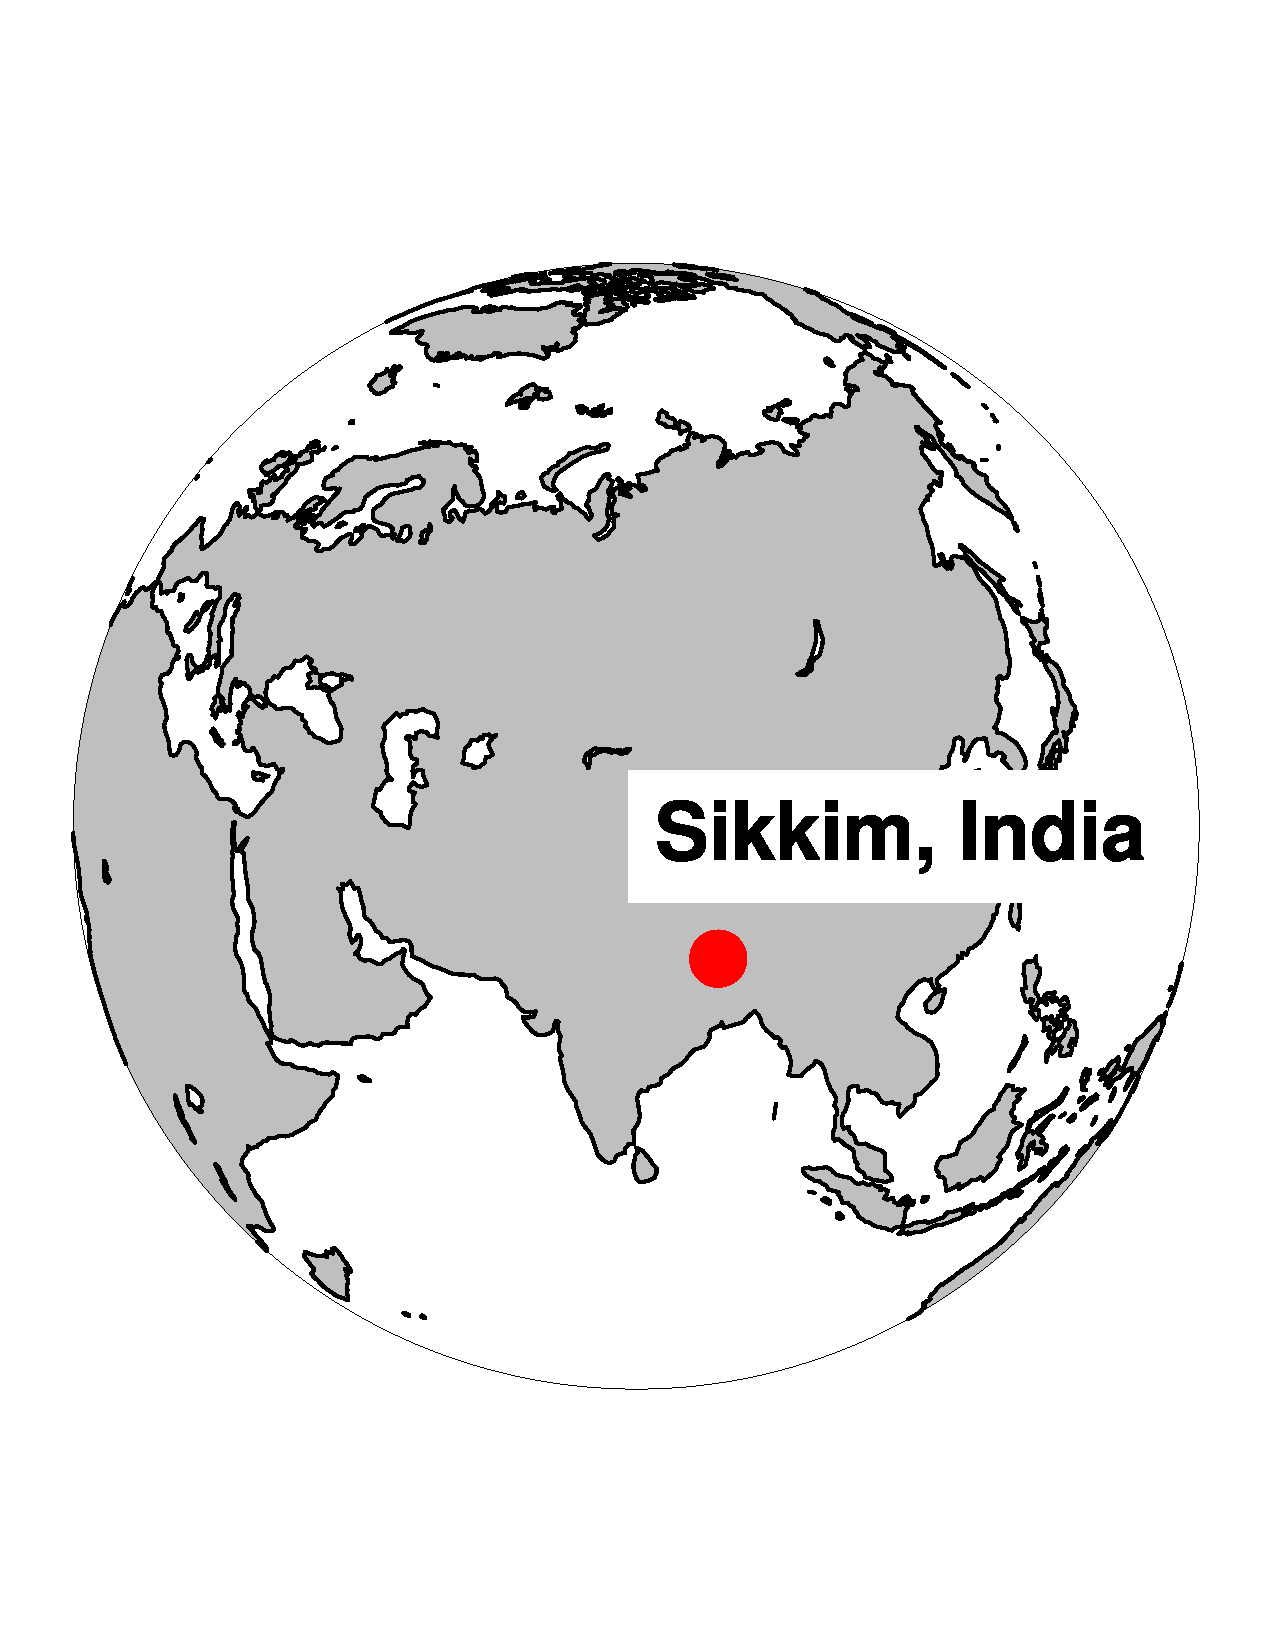
\includegraphics[width=\textwidth]{plot_maxhsurf.pdf}
          \end{minipage}
        \end{tabbing}

        \addtocounter{table}{-1} % we need this because we have a nested table-longtable environment
        \definecolor{bggreen}{cmyk}{0.38, 0.00, 0.25, 0.16 }
        \renewcommand{\baselinestretch}{1.00}\normalsize%
        \pgfkeys{/pgf/number format/set thousands separator={\,}}
        \pgfplotstableread{vertical_half_levels_maxheight_i.txt}{\loadedtable}\vspace*{0pt}%
        \pgfplotstabletypeset[ 
        begin table=\begin{longtable}, 
          end table=\end{longtable},
        columns={k,z,k,z,k,z,k,z},
        every  head row/.style={after row={\hline}},
        precision=2,
        font=\normalsize,
        columns/k/.style={column name=level idx., column type=c, 
          column type/.add={>{\columncolor{bggreen!15}}}{}},
        columns/z/.style={column name=height $[m]$, fixed,dec sep align, zerofill,precision=3},
        display columns/0/.style={select equal part entry of={0}{4},string type},
        display columns/1/.style={select equal part entry of={0}{4}},
        display columns/2/.style={select equal part entry of={1}{4},string type},
        display columns/3/.style={select equal part entry of={1}{4}},
        display columns/4/.style={select equal part entry of={2}{4},string type},
        display columns/5/.style={select equal part entry of={2}{4}},
        display columns/6/.style={select equal part entry of={3}{4},string type},
        display columns/7/.style={select equal part entry of={3}{4}},
        ] {\loadedtable}
      \end{minipage}
    };
  \end{tikzpicture}
\end{table}


\begin{table}[p]
  \caption{Height above ground~$z_i^f(x)$ (full levels) for the grid point with maximum topography height
    in the operational setup R03B07, 13\,km spatial resolution.}
  
  \vspace*{4em}
  \begin{tikzpicture}
    \node[draw,rectangle] (0,0) {
      \begin{minipage}{0.96\textwidth}
        \vspace*{4em}%
        \begin{tabbing}     
          \hspace*{3em}%
          \begin{minipage}[b]{0.55\textwidth}\vspace*{0em}%
            \underline{\textbf{Example: Height above ground, full levels}}\\[1em]
            Location with max.\ surface height\\    
            \begin{tabbing}
              \texttt{CLON}/\texttt{CLAT}   \== 88.180 / 27.938          \\[0.5em]
              \texttt{HSURF}                \>=   6425.974 m
            \end{tabbing}
          \end{minipage}
          \=\hspace*{3em}%
          \begin{minipage}[c]{0.25\textwidth}\vspace*{-8em}%
            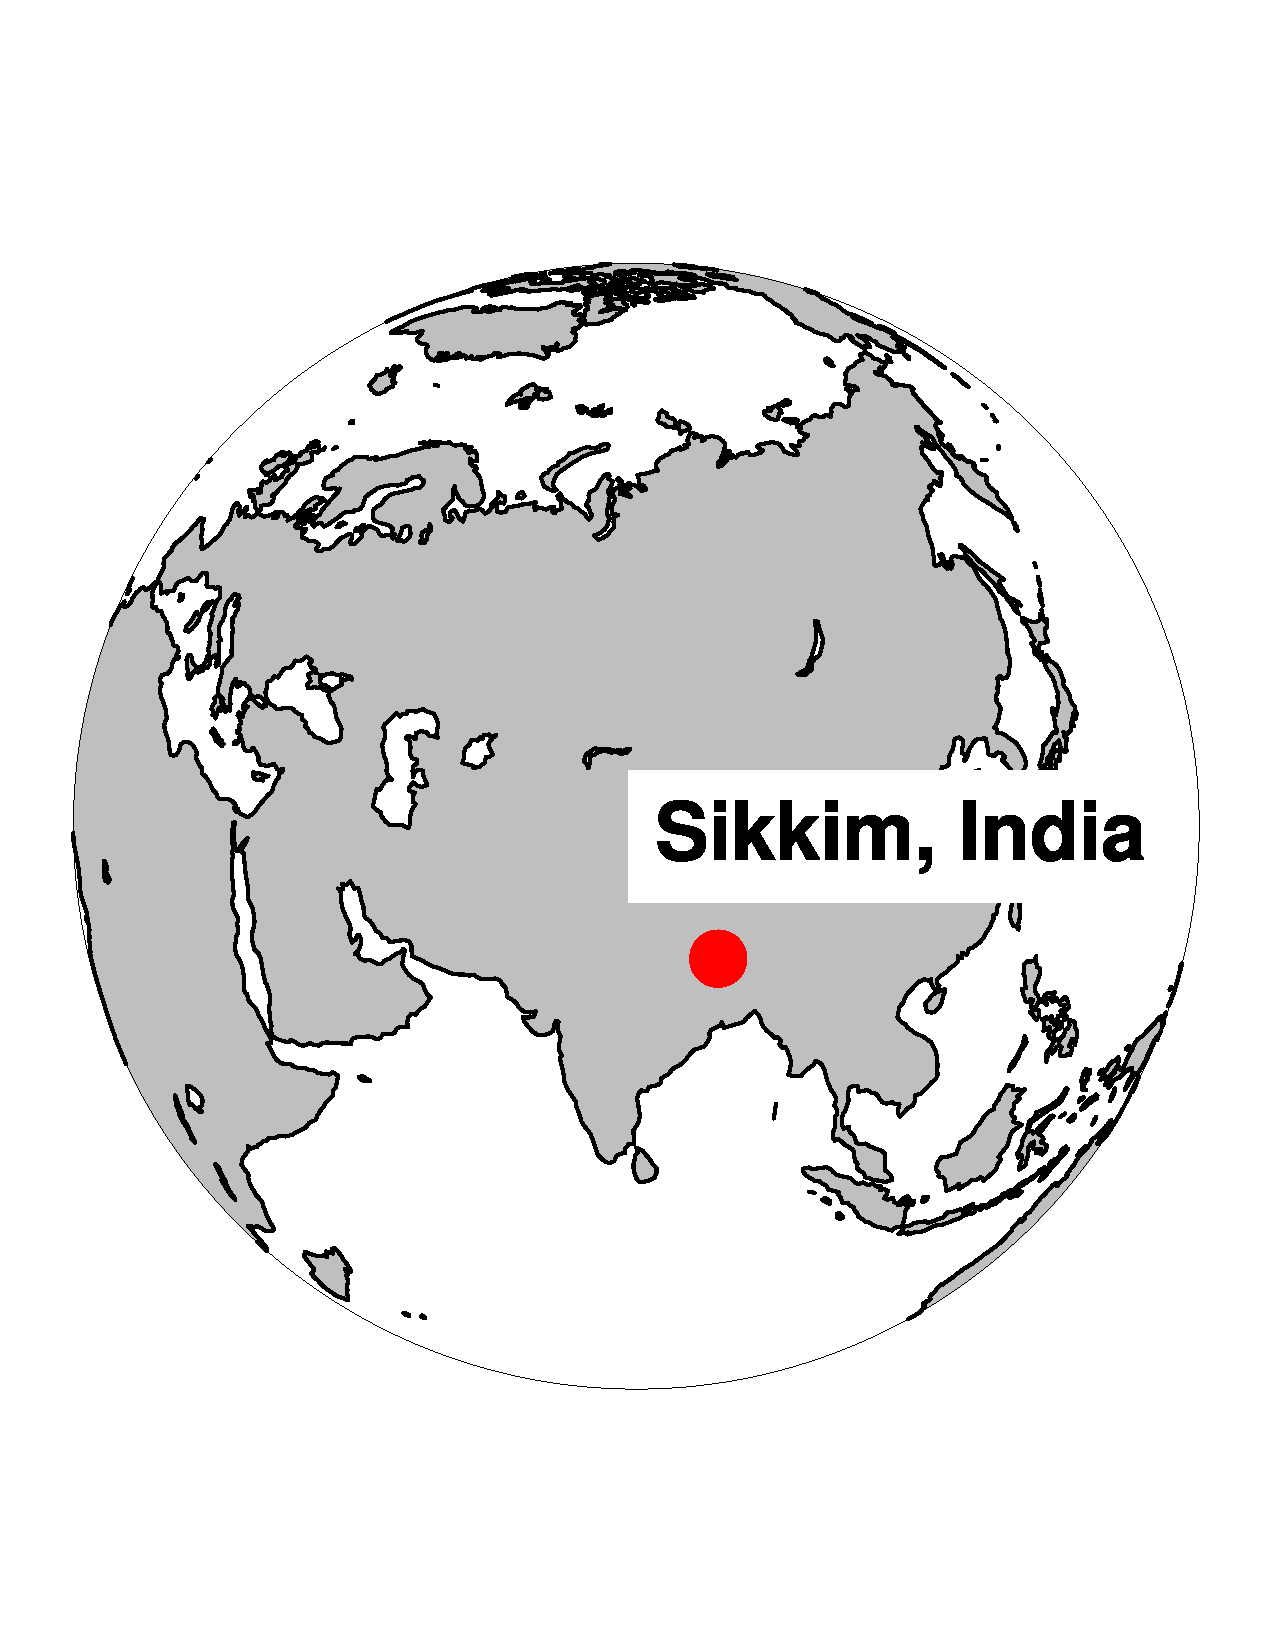
\includegraphics[width=\textwidth]{plot_maxhsurf.pdf}
          \end{minipage}
        \end{tabbing}

        \addtocounter{table}{-1} % we need this because we have a nested table-longtable environment
        \definecolor{bgblue}{cmyk}{ 0.53, 0.20, 0.00, 0.27}
        \renewcommand{\baselinestretch}{1.00}\normalsize%
        \pgfkeys{/pgf/number format/set thousands separator={\,}}
        \pgfplotstableread{vertical_full_levels_maxheight_i.txt}{\loadedtable}\vspace*{0pt}%
        \pgfplotstabletypeset[ 
        begin table=\begin{longtable}, 
          end table=\end{longtable},
        columns={k,z,k,z,k,z,k,z},
        every  head row/.style={after row={\hline}},
        precision=2,
        font=\normalsize,
        columns/k/.style={column name=level idx., column type=c, 
          column type/.add={>{\columncolor{bgblue!15}}}{}},
        columns/z/.style={column name=height $[m]$, fixed,dec sep align, zerofill,precision=3},
        display columns/0/.style={select equal part entry of={0}{4},string type},
        display columns/1/.style={select equal part entry of={0}{4}},
        display columns/2/.style={select equal part entry of={1}{4},string type},
        display columns/3/.style={select equal part entry of={1}{4}},
        display columns/4/.style={select equal part entry of={2}{4},string type},
        display columns/5/.style={select equal part entry of={2}{4}},
        display columns/6/.style={select equal part entry of={3}{4},string type},
        display columns/7/.style={select equal part entry of={3}{4}},
        ] {\loadedtable}
      \end{minipage}
    };
  \end{tikzpicture}
\end{table}  %--- Einbinden der Appendix
\end{appendices}

\backmatter
\bibliography{litera.bib} %--- Create list of references

% remove chapter number from header for Acknowledgements
\renewcommand{\chaptermark}[1] {
  \markboth{#1}{}
}

% use default again
\renewcommand{\chaptermark}[1]{%
  \markboth{\chaptername
    \ \thechapter.\ #1}{}}


% --------------------------------------------------------------------------------
% --------------------------------------------------------------------------------
%\cleardoublepage
% \section*{Database documentation: list of todos}
% --------------------------------------------------------------------------------
% --------------------------------------------------------------------------------

% \begin{itemize}
%   \item EU nest: ''Urstart'' fields must be contained in the $VV=0$ list.
%   \item lake variables: ask Dimitri if these fields could be changed
%     from RBF interpolation to nearest-neighbor.
%   \item \st{EU nest, output of wind gusts hourly until 78h, afterwards 3
%     hourly:  Output of VMAX\_10M is 3-hourly for $VV>78h$. The
%     sampling interval should also be changed to 3h after $VV>78h$.}
%   \item \st{Create two additional timing diagrams like}
%     \ref{fig:forecast_length_global} \st{for the EU nest: One illustration for
%     native grid and one for the regular output grid.}
%   \item Questions for the ICON migration group:
%         \begin{itemize}
%           \item QR, QS necessary for lon-lat?
%           \item Q\_SEDIM required?
%           \item QV\_2M (lat-lon) required?
%           \item SOBS\_RAD, THBS\_RAD (lat-lon) required?
%           \item TQC\_DIA, TQI\_DIA ?
%           \item REL\_HUM on height levels required?
%           \item CAPE\_ML required?
%           \item CAPE\_CON (lat-lon) required?
%           \item FR\_ICE (lat-lon) required?
%           \item How should DTKE\_CON be treated on the EU nest, native grid?
%         \end{itemize}
%   \item \st{Height-level interpolated pressure: L1/L2 are 102/255 in the COSMO documentation.}
%   \item DTKE\_CON: not consistent with namelist.
% \end{itemize}


\end{document}
